
%%%%%%%%%%%%%%%%%%%%%%%%%%%%%%%%%%%%%%%%%%%%%%%%%%%%
% Document type, global settings, and packages
%%%%%%%%%%%%%%%%%%%%%%%%%%%%%%%%%%%%%%%%%%%%%%%%%%%%
%\documentclass[a4paper,12pt]{book}
\documentclass[12pt]{report}   %12 point font for Times New Roman
\usepackage{bibentry}
\usepackage[edges]{forest}
\usetikzlibrary{arrows.meta}
\usepackage{amsmath}
\usepackage{amssymb}
\usepackage{bm}
%%
\usepackage{tikz}
%\usetikzlibrary{arrows}
%\usepackage{epsfig}
%\usepackage{ulem}
%\usepackage{cite}
\usepackage[algo2e,linesnumbered,ruled,vlined]{algorithm2e}
%\usepackage[boxruled,linesnumbered]{algorithm2e}
\usepackage[shortlabels]{enumitem}
\usepackage{color}
\usepackage{xspace}
\usepackage{url}
\DeclareGraphicsExtensions{.eps}
%\usepackage{amsmath}
\usepackage{lettrine}
\usepackage{algorithm,epsfig}
\usepackage[export]{adjustbox}

\usepackage{multicol}
%\usepackage{flushend}
\usepackage{fancyhdr}
\usepackage{latexsym}
\usepackage{subcaption}
\usepackage{epstopdf}
\usepackage{siunitx}
 \usepackage{booktabs,xcolor}
\usepackage{algpseudocode, setspace, amsmath,amsfonts} 
\usepackage{scalerel}
\usepackage{tikz}
\usepackage{amssymb}
\newcommand{\estimates}{\overset{\scriptscriptstyle\wedge}{H}}
\usepackage{graphicx}
\usepackage{textcomp}
%%
\usepackage{graphics} % for pdf, bitmapped graphics files
\usepackage{epsfig} % for postscript graphics files
%\usepackage{mathptmx} 
 

\usepackage{xcolor}
%\usepackage{titlesec}
\definecolor{gray75}{gray}{0.75}
\usepackage[letterpaper, left=1.5 in, right=1in, top=1in, bottom=1in]{geometry}
\usepackage{setspace}  %use this package to set linespacing as desired
\usepackage[explicit]{titlesec}  %title control and formatting
\usepackage[titles]{tocloft}  %table of contents control and formatting
\usepackage[backend=bibtex, sorting=none, bibstyle=ieee]{biblatex}  %reference manager
\usepackage[bookmarks=true, hidelinks]{hyperref}
\usepackage[page]{appendix}  %for appendices
\usepackage{rotating}  %for rotated, landscape images
\usepackage[normalem]{ulem}  %for italicized text
%\usepackage{amsmath,amssymb,amsfonts,url}
\DeclareMathOperator*{\argmax}{argmax}
%\usepackage{algorithmic}
\usepackage{color}
\usepackage{textcomp}
%%%%%%%%%%%%%%%%%%%%%%%%%%%%%%%%%%%
% Bibliography
%%%%%%%%%%%%%%%%%%%%%%%%%%%%%%%%%%%

%Add your bibliography file here
\bibliography{references}
%\bibliography{publications}
% prevent certain fields in references from printing in bibliography
\AtEveryBibitem{\clearfield{issn}}
\AtEveryBibitem{\clearlist{issn}}

\AtEveryBibitem{\clearfield{language}}
\AtEveryBibitem{\clearlist{language}}

\AtEveryBibitem{\clearfield{doi}}
\AtEveryBibitem{\clearlist{doi}}

\AtEveryBibitem{\clearfield{url}}
\AtEveryBibitem{\clearlist{url}}

\AtEveryBibitem{%
  \ifentrytype{online}
    {}
    {\clearfield{urlyear}\clearfield{urlmonth}\clearfield{urlday}}}

%%%%%%%%%%%%%%%%%%%%%%
% Start of Document
%%%%%%%%%%%%%%%%%%%%%%

\begin{document}
\doublespacing  %set line spacing


%%%%%%%%%%%%%%%%%%%%%%%%%%%%%%%%%%%%%
% Title Page
%%%%%%%%%%%%%%%%%%%%%%%%%%%%%%%%%%%%%

%% Define your thesis title, your name, your school, and your month and year of graduation here

\newcommand{\thesisTitle}{ Digital Signal Processing Algorithms for
\vspace{1\baselineskip} Multiple Input Multiple Output Based  Systems}
\newcommand{\yourName}{Farzana Kulsoom}
\newcommand{\tutorName}{Pietro Savazzi}
\newcommand{\yourSchool}{ELECTRONICS, COMPUTER SCIENCE AND ELECTRICAL ENGINEERING​ }
\newcommand{\yourMonth}{February}
\newcommand{\yourYear}{2020}

%%%%%%%%%%%%%%%%%%%%%%%%%%%%%%%%%%%%%%%%%%%%%%%%%%%%%%%%%
% Do not edit these lines unless you wish to customize
% the template
%%%%%%%%%%%%%%%%%%%%%%%%%%%%%%%%%%%%%%%%%%%%%%%%%%%%%%%%%



\begin{titlepage}
\begin{center}

\begin{singlespacing}

\textbf{\LARGE \MakeUppercase UNIVERSITA’ DEGLI STUDI DI PAVIA\\
\vspace{0.3\baselineskip}
FACOLTA’ DI INGEGNERIA }\\
%{\thesisTitle}} \\
\vspace{3\baselineskip}
{\Large CICLO  XXXII}\\
\vspace{0.5\baselineskip}
{\Large 2016-2019}\\
\vspace{1\baselineskip}
\includegraphics[width = 40mm]{logu.png}\\
\vspace{1\baselineskip}
\textbf{\LARGE  \thesisTitle}\\
A Dissertation\\
Presented to\\
The Academic Faculty\\
\vspace{3\baselineskip}
{\large By}\\
\vspace{3\baselineskip}
{\large \yourName}\\
\vspace{1\baselineskip}
{\large Tutor: \hspace{0.3pt}\tutorName}\\
\vspace{3\baselineskip}
In Partial Fulfillment\\
of the Requirements for the Degree\\
Doctor of Philosophy in the\\
{ \large Department of \yourSchool}\\

%UNIVERSITA’ DEGLI STUDI DI PAVIA
 
\vspace{\baselineskip}
\yourMonth{} \yourYear{}
\vfill
Copyright \copyright{} \yourName{} \yourYear{}

\end{singlespacing}

\end{center}
\end{titlepage}



\currentpdfbookmark{Title Page}{titlePage}  %add PDF bookmark for this page

%%%%%%%%%%%%%%%%%%%%%%%%%%%%%%%%%%%%%
% Approval Page
%%%%%%%%%%%%%%%%%%%%%%%%%%%%%%%%%%%%%
%% Define your committee members. If you have less than 6, simple delete/comment the unused lines

\newcommand{\committeeMemberOne}{Prof. Pietro Savazzi, Advisor}
\newcommand{\committeeMemberOneDepartment}{Department of Electronic and Computer Science and Electrical Engineering}
\newcommand{\committeeMemberOneAffiliation}{University of Pavia, Italy}

\newcommand{\committeeMemberTwo}{Prof.Magarini Maurizio}
\newcommand{\committeeMemberTwoDepartment}{Department of Electronics, Informatics and BioEngineering}
\newcommand{\committeeMemberTwoAffiliation}{Politecnico di Milano, Italy}

\newcommand{\committeeMemberThree}{Prof. Laura Galluccio}
\newcommand{\committeeMemberThreeDepartment}{Department of Electrical, Electronic and Computer Engineering}
\newcommand{\committeeMemberThreeAffiliation}{University of Catania, Italy}

\newcommand{\committeeMemberFour}{Dr. Four}
\newcommand{\committeeMemberFourDepartment}{School of Computer Science}
\newcommand{\committeeMemberFourAffiliation}{Georgia Institute of Technology}

\newcommand{\committeeMemberFive}{Dr. Five}
\newcommand{\committeeMemberFiveDepartment}{School of Public Policy}
\newcommand{\committeeMemberFiveAffiliation}{Georgia Institute of Technology}

\newcommand{\committeeMemberSix}{Dr. Six}
\newcommand{\committeeMemberSixDepartment}{School of Nuclear Engineering}
\newcommand{\committeeMemberSixAffiliation}{Georgia Institute of Technology}

\newcommand{\approvalDay}{11}
\newcommand{\approvalMonth}{January}
\newcommand{\approvalYear}{2000}

%%%%%%%%%%%%%%%%%%%%%%%%%%%%%%%%%%%%%%%%%%%%%%%%%%%%%%%%%
% Do not edit these lines unless you wish to customize
% the template
%%%%%%%%%%%%%%%%%%%%%%%%%%%%%%%%%%%%%%%%%%%%%%%%%%%%%%%%%


\begin{titlepage}
\begin{singlespacing}
\begin{center}

\textbf{\large {Thesis Title: \thesisTitle}}\\
\vspace{10\baselineskip}

\end{center}
\vfill

%Define minipages, depending on how many authors there are
\ifdefined\committeeMemberFour

Approved by:
\vspace{2\baselineskip}		%adjust the number in front of "\baselineskip" for alignment

\begin{minipage}[b]{0.4\textwidth}
	
	\committeeMemberOne\\
	\noindent\rule{6cm}{0.4pt}\\
	\committeeMemberOneDepartment\\
	\textit{\committeeMemberOneAffiliation}\\
	
	
	\committeeMemberTwo\\
	\noindent\rule{6cm}{0.4pt}\\
	\committeeMemberTwoDepartment\\
	\textit{\committeeMemberTwoAffiliation}\\
	
	\committeeMemberThree\\
	\noindent\rule{6cm}{0.4pt}\\
	\committeeMemberThreeDepartment\\
	\textit{\committeeMemberThreeAffiliation}\\
	
	\vspace{2\baselineskip}		%adjust the number in front of "\baselineskip" for alignment
	
\end{minipage}





\end{singlespacing}
\end{titlepage}



%%%%%%%%%%%%%%%%%%%%%%%%%%%%%%%%%%%%%
% Epigraph
%%%%%%%%%%%%%%%%%%%%%%%%%%%%%%%%%%%%%

\input{epigraph.tex}

%%%%%%%%%%%%%%%%%%%%%%%%%%%%%%%%%%%%%
% Dedication
%%%%%%%%%%%%%%%%%%%%%%%%%%%%%%%%%%%%%

% Define your dedication statement here

\newcommand{\yourDedication}{I would like to dedicate this thesis to my loving parents, my supportive husband and
my wonderful daughters}

%%%%%%%%%%%%%%%%%%%%%%%%%%%%%%%%%%%%%%%%%%%%%%%%%%%%%%%%%
% Do not edit these lines unless you wish to customize
% the template
%%%%%%%%%%%%%%%%%%%%%%%%%%%%%%%%%%%%%%%%%%%%%%%%%%%%%%%%%

\begin{titlepage}
\begin{center}

\vspace*{\fill}
\yourDedication\\
\vspace*{\fill}

\end{center}
\end{titlepage}


%%%%%%%%%%%%%%%%%%%%%%%%%%%%%%%%%%%%%
% Acknowledgments
%%%%%%%%%%%%%%%%%%%%%%%%%%%%%%%%%%%%%

\pagenumbering{roman}
\addcontentsline{toc}{chapter}{Acknowledgments}
\setcounter{page}{5} % set the page number appropriately based on the number of intro pages
\clearpage
\begin{centering}
\textbf{ACKNOWLEDGEMENTS}\\
\vspace{\baselineskip}
\end{centering}

%Insert your dedication text here
First and foremost, I am grateful to God for blessing me with good health, vitality, and strength to accomplish this goal which I ever dreamed of. \\
I extend my sincerest gratitude to my supervisors,  Prof. Pietro Savazzi for his guidance and encouragement during the entire period of Ph.D. I am especially thankful to him for his thought-provoking assistance to solve the research problem. His guidance, knowledge, and expertise have improved my research skills, ability to think critically and deal with challenging situations. I am privileged and I consider myself lucky to be his research student. I am also very thankful to Anna Vizziello for assisting me in my research work. The guidance and assistance which she has provided, including suggestions, reviewing my papers, making modifications, keeping my morale high and all her nice and warm words are ineffable and it improved my technical and research skills.  \\
Particularly, many thanks to  Prof. Fabio Dell'Acqua for his support and help during the time of my Ph.D. I have learned many things from him including methodologies of scientific research as well as analytical and critical thinking.  All these will surely benefit me throughout my career.
I am grateful to Prof. Lorenzo Favalli and Paolo Gamba for reviewing my work during lab meetings and providing valuable suggestions and feedback.  \\
Finally, my family support without which I would never be able to achieve this goal.  My parents who prayed for me and encouraged me for doing this work. My caring and supportive husband who cheered me during a tough time,  restored me and kept me moving when it seemed difficult. My lovely daughters Fatimah, Hanniyah, and Malikha, my inlaws who always boosted me when I was feeling low. 

\clearpage
%\pagenumbering{gobble}  %remove page number on summary page


\addtocontents{toc}{\cftpagenumbersoff{chapter}} 

%\currentpdfbookmark{Acknowledgments}{acknowledgments}
%\addtocontents{toc}{\cftpagenumberson{chapter}} 

%%%%%%%%%%%%%%%%%%%%%%%%%%%%%%%%%%%%%
% Table of Contents
%%%%%%%%%%%%%%%%%%%%%%%%%%%%%%%%%%%%%

% Format for Table of Contents
\newcommand{\hsp}{\hspace{0pt}}
\renewcommand{\cftchapdotsep}{\cftdotsep}  %add dot separators
\renewcommand{\cftchapfont}{\bfseries}  %set title font weight
\renewcommand{\cftchappagefont}{}  %set page number font weight
\renewcommand{\cftchappresnum}{Chapter }
\renewcommand{\cftchapaftersnum}{:}
\renewcommand{\cftchapnumwidth}{5em}
\renewcommand{\cftchapafterpnum}{\vskip\baselineskip} %set correct spacing for entries in single space environment
\renewcommand{\cftsecafterpnum}{\vskip\baselineskip}  %set correct spacing for entries in single space environment
\renewcommand{\cftsubsecafterpnum}{\vskip\baselineskip} %set correct spacing for entries in single space environment
\renewcommand{\cftsubsubsecafterpnum}{\vskip\baselineskip} %set correct spacing for entries in single space environment

%format title font size and position (this also applys to list of figures and list of tables)
\titleformat{\chapter}[display]
{\normalfont\bfseries\filcenter}{\chaptertitlename\ \thechapter}{0pt}{\MakeUppercase{#1}}

\renewcommand\contentsname{Table of Contents}

\begin{singlespace}
\tableofcontents
\end{singlespace}

\currentpdfbookmark{Table of Contents}{TOC}

\clearpage

%%%%%%%%%%%%%%%%%%%%%%%%%%%%%%%%%%%%%
% List of figures and tables
%%%%%%%%%%%%%%%%%%%%%%%%%%%%%%%%%%%%%

\addcontentsline{toc}{chapter}{List of Tables}
\begin{singlespace}
	\setlength\cftbeforetabskip{\baselineskip}  %manually set spacing between entries
	\listoftables
\end{singlespace}

\clearpage

\addcontentsline{toc}{chapter}{List of Figures}
\begin{singlespace}
\setlength\cftbeforefigskip{\baselineskip}  %manually set spacing between entries
\listoffigures
\end{singlespace}

\clearpage

%%%%%%%%%%%%%%%%%%%%%%%%%%%%%%%%%%%%%%%%%%%%%%%%%%%%%%%%%%%%%%%%%
% This is the Summary (abstract should be separate document)
%%%%%%%%%%%%%%%%%%%%%%%%%%%%%%%%%%%%%%%%%%%%%%%%%%%%%%%%%%%%%%%%%

\clearpage
\begin{centering}
\textbf{SUMMARY}\\
\vspace{\baselineskip}
\end{centering}

The evolution of wireless communication brought several innovative technologies, Multiple Input Multiple Output(MIMO) system is one of such technology which gained popularity due to its capability to enhance spectral efficiency and reliability.  Although, MIMO aides enhancing system capacity and performance, however, it is challenging due to the high number of antennas at a transmitter and serving large numbers of users simultaneously.  It has been therefore the popular area of research in the last decade, meeting ever-increasing demands of data rates.   Nevertheless, severing multiple terminals simultaneously is challenging due to interference among them. The main goal of this research is to mitigate interference among users,  gain better energy and spectral efficiency by employing different DSP based algorithms using MIMO communication paradigm. \\
In this thesis, we have investigated different MIMO based research problems to enhance throughput, which is essentially achieved by mitigating inter-terminal interference by employing directional beams. To employ a directional beam it is imperative to have channel knowledge, which can be accomplished by performing channel estimation. This estimate can be achieved by using time or frequency duplexing, although, with an increased number of antennas in large scale MIMO (massive MIMO), the problem becomes more complicated in both types of duplexing schemes. The predicament can be addressed properly if the high dimensional signal is reduced to a low dimension by taking the compressive sensing(CS) paradigm into account. A framework is proposed to reduce training and feedback overhead by considering the MIMO channel as sparse in mobile communication.  Another important problem in the modern communication system is of phase recovery,  a reduced complexity Kalman filtering based solution is proposed to address the phase recovery problem in XPIC systems. Further, a novel method is devised that allows multiple implants in the intra-body network to communicate in an energy-efficient manner. 
The comparison with state of the art methods is also exhibited. The research work conducted in this thesis addresses theoretical, methodological and empirical contributions to MIMO based system research problem and attempted to achieve better performance by employing different digital signal processing(DSP) based algorithms.

%%%%%%%%%%%%%%%%%%%%%%%%%%%%
%
% Chapters
%
%%%%%%%%%%%%%%%%%%%%%%%%%%%%

%%%%%%%%%%%%%%%%%%%%%%
% formatting
%%%%%%%%%%%%%%%%%%%%%%

% resume page numbering for rest of document
\clearpage
\pagenumbering{arabic}
\setcounter{page}{1} % set the page number appropriately

% Adjust chapter title formatting

%\titleformat{\chapter}[display]{\flushright
%\fontseries{b}\fontsize{80}{100}\selectfont}{\fontseries{b}\fontsize{100}{130}\selectfont \textcolor{gray75}\thechapter\hsp}{0pt}{\\ \Huge\bfseries}[]


\titleformat{\chapter }[display]
{\normalfont\bfseries\filleft}{\MakeUppercase\chaptertitlename\ \thechapter}{0pt}{\MakeUppercase{#1}}[\vspace{2ex}\titlerule]  %spacing between titles
%\titleformat{\chapter}[display]
%{\normalfont\huge\bfseries}{\chaptertitlename\ \thechapter}{20pt}{\Huge}[\vspace{2ex}\titlerule]

\titlespacing*{\chapter}
  {0pt}{0pt}{30pt}	%controls vertical margins on title
 % \noindent\makebox[\linewidth]{\rule{\paperwidth}{0.4pt}}
% Adjust section title formatting
\titleformat{\section}{\normalfont\bfseries}{\thesection}{1em}{#1}

% Adjust subsection title formatting
\titleformat{\subsection}{\normalfont}{\uline{\thesubsection}}{0em}{\uline{\hspace{1em}#1}}

% Adjust subsubsection title formatting
\titleformat{\subsubsection}{\normalfont\itshape}{\thesubsection}{1em}{#1}

%%%%%%%%%%%%%%%%
% Chapter 1
%%%%%%%%%%%%%%%%
\pagestyle{headings}

%\chapter{Introduction and Background}
%\textcolor{red}{chapter 1 is Ready to revised}\\
Over the last few decades wireless networks have been established as one of the promising technology to provide communication with the ease of mobility and data reliability. The ever increasing demand for data rate and connectivity anywhere, anytime are the main motivations \textcolor{black}{for an intensive use of multi-antenna communication systems.} By deploying Multiple-Input Multiple-Output (MIMO) system, where multiple antennas are installed at both transmitter and receiver, it is possible to increase the capacity and efficiency \textcolor{black}{of wireless networks with respect to more conventional Single-Input Single-output (SISO) based systems}. MIMO systems are one of the keystones in the development and extension of data-intensive applications like  and social  media and video streaming on hand held devices, surveillance and navigation systems for target detection and tracking, also health based applications using intra-body communications (IBC).\\
However, this improvement in performance gain and reliability also \textcolor{black}{increases processing and hardware costs and creates new challenges. Therefore, the requirement to develop efficient digital signal processing (DSP) based algorithms and multiple access techniques is indispensable to tackle this challenge.}
\section{Background}
The main challenges to enhance system performance in communication system \textcolor{black}{derive from \textit{fading} which is due to changes in transmission medium or paths which cause time variation of received signal power, and \textit{interference,} mainly caused by the fact that more than one user share the same radio resources at the same time.} In more details, transmitted signals can reach the receiver by more than one paths because of scatters and obstacles in the medium, this phenomena is called multipath \textcolor{black}{interference. %Undoubtedly, to improve the system performance either we should built some techniques to avoid interference or by making signals orthogonal within the given spectrum. Multipath propagation of radio signals from transmitter to receiver results in diverse spatial characteristics. 
MIMO systems may be designed to counteract this multipath radio arrangement, resulting in better performance and reliability.}
To increase system reliability and data rate in MIMO system, two types of data transmission arrangement are generally used. In \textit{transmit/receive diversity} identical data is transmitted/received by multiple antennas, \textcolor{black}{improving signal reliability, while keeping the same system throughput. Different types of MIMO architectures are shown in figure \ref{mimo}.
\begin{figure}
\includegraphics[scale=0.8]{figures/MIMO.png}
\caption{Diversities in Multi-terminal system}
\centering
\label{mimo}
\end{figure}
On the other hand, if independent data streams are transmitted from each antenna, MIMO systems could effectively increase the system throughput. In this case, the scheme is called space division multiple access (SDMA) or multi-user MIMO (MU-MIMO).}
%The MIMO systems are developed by considering existing spectrum resources, 

%\textcolor{black}{COMMENT: I think the following remaining part of this chaper needs to be modified. I think that these details on MIMO must be insterted in a more specific chapter (for instance the next chaper on wireless comms). I think you need to generally introduce the other topics of the thesis, like CS, channel recovery, intrabodyc comms, by trying to consider all of them under the main topic of MIMO communications}
Since spectrum is a limited and expensive resource it must be utilized efficiently. \textit{Spectral efficiency} determine the rate of information transmitted per unit bandwidth. Another important metric to keep in mind other than spectral efficiency  while measuring performance in wireless system is \textit{energy efficiency (EE)}. Energy efficiency can be achieved by optimizing the transmit power.
To mitigate interference across multiple users in MU-MIMO different types of \textit{beamforming or precoding} techniques can used at transmitter: 
\begin{itemize}
    \item \textbf{Analog Beamforming:} In analog beamforming, analog phase shifters are used to steer the beam in the direction of the user \cite{bjornson_book}. Multiple beams can be formed to serve different users, but it depends on number of antennas and size of array used \cite{thesis_xiang}. To serve different users simultaneously, the possible beams that can be formed must be orthogonal to each other, a limiting factor to analogue beamforming.
    \item \textbf{Digital beamforming/Precoding:} The digital beamforming or linear precoding, is performed in baseband \textcolor{black}{ where the different user signals are }superimposed with varying power and phase. Digital beamforming is more flexible and simple \textcolor{black}{than} analog beamforming, and its complexity does not grow with the number of antennas.
\end{itemize}

\section{Compressed Sensing}
\textcolor{black}{Due to multiple nodes, MIMO systems are computationally expensive and their energy requirement is also high. The main reason \textcolor{black}{is the }high level of signal processing techniques \textcolor{black}{needed }to mitigate interference among nodes as they are sharing channel resources. \textcolor{black}{Moreover,} the transmitter and receiver design become complicated to manage multi-antenna transmission. \textcolor{black}{These issues} can be handled, if we will be able to reduce the \textcolor{black}{signal }measurements with the help of some signal processing techniques. Compressive sensing (CS)  techniques \textcolor{black}{allow to } recover \textcolor{black}{a} signal with a much lower number of linear measurements than in the conventional case. \textcolor{black}{If respecting} the constraint that the underlying signal is sparse. \textcolor{black}{In this way},  the system can be made energy-efficient \textcolor{black}{by exploring the} underlying signal. Numerous examples can be given for signals which are sparse in some \textcolor{black}{particular domain like} time, frequency \textcolor{black}{and wavelet ones.} In the following, two real-world sparse signal cases are explained \textcolor{black}{in order to solve} some MIMO based problems \textcolor{black}{discussed in this thesis}.
\begin{itemize}
    \item \textcolor{black}{In} massive MIMO \textcolor{black}{system }most of the channel energy lies only on few dominant taps \cite{sparse_channel}, therefore its channel impulse response (CIR) will be sparse. This is due to the large number of antennas at the base station (BS) with only few scatters at the BS side (compared to the number of antennas), hence only  few active transmission directions per user, hence the channel matrix tends to be sparse \cite{mainref-joint,exp-vitual}.
\item \textcolor{black}{For} humans in intra-body communications (IBC) system efficiency is directly related to the energy \textcolor{black}{consumption} and security related issues.
In practical applications, implants may not transmit data
continuously. Hence, we can easily assume that the sensed data is sparse, and with the help of the CS framework sufficient energy efficiency can be achieved, without degrading the performance.
\end{itemize}
\section{\textcolor{black}{MIMO Applications} }
In this thesis three \textcolor{black}{MIMO} applications have been considered and their \textcolor{black}{related} research problems have been solved with the help of signal processing techniques.
 \subsection{Massive MIMO}
 Massive MIMO or large scale MIMO is a natural extension of conventional MIMO, \textcolor{black}{and} it groups large number of antennas at \textcolor{black}{the }BS to improve spectral efficiency and throughput in mobile communication. By employing large number of antennas at BS,  the system capacity is increased tremendously, because of spatial multiplexing techniques \textcolor{black}{and }higher data rates can be achieved. Beamforming techniques help massive MIMO \textcolor{black}{systems} in getting better area coverage by \textcolor{black}{optimizing the} received signal power. Moreover, it reduce the latency by using parallel detection\cite{latency} and by combating fading dips with the help of optimal beamforming \cite{magazine_eric}.
 Due \textcolor{black}{to} immense benefits of MIMO systems, \textcolor{black}{they have} become essential  part of many latest standards \textcolor{black}{such as} WLAN (802.11n, 802.11ac etc.), WiMAX (IEEE 802.16e), LTE, LTE-Advanced, etc.
 \subsection{MIMO in Intra-Body Communication}
  Intra-body communication (IBC), is a data communication technique in which human body is used as a \textcolor{black}{transmission medium} or channel. Multiple implants are embedded into the human body \textcolor{black}{in order to} sense and forward their data to \textcolor{black}{a} skin node, called relay. These implants are interconnected and work in a MIMO fashion that allows internal physiological data to be gathered in real time and analyzed offline, thereby, transforming personalized medicine.
   The theoretical background can be developed for
   beamforming using an array of implants acting as distributed MIMO antennas. Significant performance gain can be achieved with the help of beamforming techniques in IBC. However, there are several challenges associated with IBC \textcolor{black}{, like} for example, energy efficiency, interference among implants, synchronization issues, etc.  
 \subsection{Cross-polarization interference canceller (XPIC)} 
   In the evolution of fifth-generation (5G) \textcolor{black}{mobile} communication technologies, there is always an increasing demand for user traffic, resulting in higher bandwidth requirement.
Cross polarization interference cancellation (XPIC) technology
represents the enabler for dual-polarized transmissions over the
same radio frequency (RF) channel, so that the link capacity is
doubled by using two orthogonal polarization channels over the
same link. In cross-polar transmission \textcolor{black}{the} 
same carrier frequency is utilised for simultaneous
transmission/reception of two different data streams.
Basically, \textcolor{black}{one} antenna is sending information on the same carrier, \textcolor{black}{by exploiting different horizontal and vertical} polarizations. The \textcolor{black}{considered} XPIC transmission is based on two independent and unsynchronized transceiver paths for backhaul links, with completely independent transmitter and receiver local oscillators (LOs).   }
 
%The key advantages in general MIMO based system compared to SISO based system are:
%\begin{itemize}
%    \item Increase capacity, because of spatial multiplexing techniques in MIMO higher data rates can be achieved.
   % \item Reliability, in MIMO system with the help of diversity and better digital signal processing algorithm data reliability is improved.
 %   \item Better area coverage is achieved by deploying BF(beamforming), which provide optimal received signal power.
 %   \item Reduced fading effects by employing different diversity techniques in frequency, time and space.
%    \item Reduced latency by using parallel detection  \cite{latency} and by combating fading dips with the help of optimal beamforming \cite{magazine_eric}.
%\end{itemize}
%Because of immense benefits MIMO system it has already been standardized in latest wireless standards namely, WLAN (802.11n, 802.11ac etc.), WiMAX (IEEE 802.16e), LTE, LTE-Advanced etc.
%MIMO system benefits can be extended by employing more antennas at the transmitter, a natural extension of MIMO system, massive MIMO.
\section{Problem Description and Main Contribution}
This research is devoted to the analysis of MIMO based system challenges and to the development of robust algorithms and techniques to handle them. We have considered different types of MIMO system research problems.
\begin{enumerate}
\item \textbf{Channel Estimation:}
Firstly, to overcome the limitation of traditional \textcolor{black}{architecture}, large scale MIMO or massive MIMO has been proposed in \cite{mimo_eric1,mimo_eric2}. Massive MIMO not only improves the spectral and energy efficiency but also helps to mitigate inter-user interference \cite{mimo-gain}. Although, massive MIMO  solves many traditional MIMO problems, but it opens completely new research avenues. 
In more detail, with a large number of transmit antennas at BS in massive MIMO, the degree of freedom is also increased, making the system more reliable and robust with reduced error rate and high throughput. With promising throughput, it is also expected that massive MIMO can serve many users simultaneously. However, supporting multiple users simultaneously is challenging due to inter-user interference, that can be mitigated if each user has its aligned beam, which can be attained with beamforming/precoding \footnote{by beamforming we are always referring digital beamforming}. 
Uplink (UL) combining or downlink (DL) transmit beamforming require good channel state information (CSI) \textcolor{black}{ that} can be attained using time division duplex (TDD) or frequency division duplex (FDD). \textcolor{black}{In TDD scheme channel reciprocity can be used to estimate downlink channel via uplink training. However, in TDD with large number of transmit antennas, base station is assumed to serve more users simultaneously which produces severe problem of pilot contamination because of the utilization of non-orthogonal pilots \cite{mimo_eric2}. Although FDD do not enjoy this channel reciprocity, as UL and DL are in separate band but it is generally considered more robust to delay-sensitive applications \cite{FDD_or_TDD}. Moreover, most of the existing systems are \textcolor{black}{employing} FDD, therefore it is of great importance \textcolor{black}{investigating } different approaches to obtain CSI in FDD.}\\
     In FDD massive MIMO channel estimation, the main problem is the pilot training and feedback overhead which increases with the number of transmit antennas, compromising the advantages of massive MIMO \cite{Dict_learning}.
     Therefore, pilot training \textcolor{black}{and feedback overhead} reduction techniques have been presented and \textcolor{black}{compared} with the existing research works. The results show that \textcolor{black}{the proposed} system outperform existing schemes.
    % Moreover, in addition to pilot overhead reduction technique algorithmped for limited feedback in a partially joint channel.The comparison has been carried out with state of the art algorithms, and results shows that our presented system is more efficient than previously proposed one. 
 \item \textbf{Synchronization:} We have considered the issues related to synchronization in MIMO based systems \textcolor{black}{developing such techniques for } cross-polarization interference cancelling (XPIC) system. Reduced complexity Kalman based algorithms are proposed to recover the phase of XPIC receiver in microwave radio relay links.
 %For the fulfillment of high data rate demand, accurate and realizable synchronization and beamforming techniques are indispensable.  With the help of such synchronization techniques,  MIMO system can achieve a higher link capacity by using higher-order modulation schemes(i-e QAM)\cite{our_kalman}. For that reason, we have considered XPIC, or
 \textcolor{black}{\item \textbf{Beamforming Galvanic Coupling Signals:}\\
 The state of the art for Intra-Body Communication (IBC) relies on high frequency radio (RF) signals. RF based systems are not energy efficient \textcolor{black}{from the point of view of } IBC. Additionally, emitted RF signals may extend to several feet around the body, creating privacy risks. We employed an alternative wireless architecture for IBNs using galvanic coupling (GC), in which low or medium frequency ($100\,\mathrm{kHz}$-$1\,\mathrm{MHz}$) and weak ($\leq 1\,\mathrm{mW}$) electrical currents are modulated with data and directly coupled to the tissue. The privacy risks related to RF are eliminated by using GC in IBNs since the signals do not propagate outside the skin layer \cite{teshome}. In GC based system currents are used in place of classical radio frequency (RF) links.\\
 As the first step, we devise a
method that allows multiple implants to communicate individual
sensed data to each other through code division multiple access (CDMA) combined with compressive sensing (CS) method to
lower the transmission time and save energy, as well as delegates
the computational burden of despreading and decoding only
to the on-body surface relays. Then, we devise a distributed
beamforming approach that allows coordinated transmissions
from the implants to the relays by considering the specific tissue
path chosen and tissue heating-related safety constraints.We then
proceed to implement distributed beamforming on a phantom of
human tissue and prove an increase in received signal strength
and decrease in BER due to constructive interference of the
signals of each implant.}
\end{enumerate}

\section{Thesis Organization}
%\textcolor{black}{COMMENT: please replace "we have" with a more formal in third person, in all the following sentences}
%\textcolor{olive}{ done}\\
{The Chapter 2}, presents MIMO system in general and the theoretical underpinnings of MU-MIMO. Also, the assumptions and challenges while dealing with channel estimation in  MIMO are discussed.\\
%ofdm, types of beamforing, equalization
{The Chapter 3}, presents a brief introduction to the essentials of compressive sensing theory in context of sparse channel estimation and most widely used sparse signal recovery algorithms.\\
%signal recovery, sensing matrix,algorithm classification 1)greedy algorithms and convex optimizatio based,
{The chapter 4}, covers the pilot reduction techniques for sparse channel estimation in massive MIMO systems. We exploit compressive sensing (CS) techniques to accurately estimate the channel, while assuring overhead reduction which is proportional to the sparsity level of the channel. 

{The Chapter 5}, have discussed joint Sparse Channel Recovery with Quantized feedback for Multi-User Massive MIMO Systems. In this chapter, a distributed compressed sensing based novel algorithm, 2-step quantized partially joint orthogonal matching pursuit (Q-PJOMP) is proposed which not only reduce training overhead but also recover the channel from limited feedback for FDD based multi-user massive MIMO.

{In chapter 6}, a novel method is  devised that allows multiple implants in intra-body network to communicate individual sensed data to each other through code division multiple access (CDMA) combined with compressive sensing (CS) method to lower the transmission time and save energy and lower computational burden.

{In chapter 7}, the research work is presented on galvanic coupling (GC) technology.A sound card based GC testbed is designed and implemented to achieve  high flexibility and real time physiological data sets transmissions.

{Chapter 8}, discussed the reduced complexity Kalman filtering for phase recovery in XPIC systems. In this work, two completely independent radio frequency (RF) transceiver chains are considered for the two different polarization's, in order to have the maximum flexibility to connect different single carrier transceivers to dual-polarized antennas.\\

%\textbf{In chapter 10}, the issue of multipath interference in multi-receiver FMCW RADAR is investigated for multi-layer snow-pack.





%beamforming helps us to take the advatge of spatial muliplexing(pararel channels in space) without interferece.


%TDD and FDD difference  Realizing massive MIMO with Time Division Duplexing (TDD) operation is convenient, due to the inherent Uplink-Downlink (UL-DL) channel reciprocity [2]. In contrast, channel reciprocity does not hold in Frequency Division Duplexing (FDD) operation, since UL and DL take places in different bands, which are separated by much more than the fading coherence bandwidth. Therefore, the UL channel state information (CSI) can not be used for DL data transmission, so that the BS has to probe the DL channel via training and ask for CSI feedback from the users\cite{FDDvsTDD}.












%%%%%%%%%%%%%%%%
% Chapter 2
%%%%%%%%%%%%%%%%

%\chapter{Overview of Wireless Communication}
\textcolor{black}{Wireless channels may be classified according to different  characteristics of propagation environments, i.e., the media in which the radio signal can propagate in the form of electromagnetic waves.} Different types of propagation channels are indoor, outdoor (urban, suburban), underwater, orbital propagation environments or any other medium in which signals propagate like, for example, the human body in intra-body communication(IBC).
%In fact   any medium where signal can propagate in a distinct fashion can be defined as channel , for example, intra body communication or snowpack has its own distinct set of challenges in terms of wireless communication.
In order to model  and define aforesaid channels , channel models are build with attributes taken from real time calculations. \\
To develop better understanding, it is essential to know that what kind of effects the channels will exert on the signal therfore, the radio wave propagation modelling is studied.
The radio waves which are generated by local disturbance in the electric and magnetic fields, spread out in all direction with distance. 
The propagation of these waves depend on medium characteristics. For example, if the propagation medium is homogeneous(i.e.  air), it will spread out uniformly in all directions and the power of the signal is attenuated with distance. However, if the medium has some sort of obstacle such as buildings, trees, mountains etc, it can undergo several attenuating effects such as reflection, refraction and scattering;  \\
-	reflection, when a wave collides any object and get reflected either completely back or at tilted angle, this changes the phase of the signal as well as it magnitude. \\
-	refraction, this effect is experienced when the wave travels from one medium to another. Refraction effects frequency and phase of the wave.\\
-	Scattering, when the wave collides at the edges of very large object the amplitude and phase of the wave is change, single wave can results into multiple waves. 

The aforesaid channel effects produce multiple paths in the channel each having its own amplitude and phases. These multiple copies of the signal interfere with each other when received on the receiver also known as multipath fading. 
%. When the distance between the transmitter and DF array is large, the contribution of these error is limited. Hence, gross errors are observed mostly due to the near-field multipath components.
There are two main categories of fading, large scale fading and small scale fading.
\begin{itemize}
    \item In large scale fading the averaged signal-power is attenuated by traveling over a long distance known as \textit{path loss} and it has larger scatters(buildings) in its paths causing a shadowing zone.
    \item Small scale fading is due to rapid fluctuations in signal amplitude or phase or because of superposition of multipath components which cause changes in amplitude and phase over a short period of time(in seconds).
    Small scale fading can be further divided into two, based on delay spread(channel response to a short pulse on multipath) and Doppler spread(frequency range over which the received doppler spectrum must be non-zero).Different types of small scale fading  is as shown in figure \ref{lb_sm_fadd}.
   
\end{itemize}
\begin{figure}
\scalebox{0.72}{
\begin{forest}
  for tree={
    font=\small\sffamily,
        draw, rounded corners,
        text centered,
        minimum height=3ex,
        text width=29ex,
        inner sep=0.5ex,
        anchor=north,
        rounded corners,
        top color=white,
        bottom color=white!20,
    l sep=5mm,
    s sep=4mm,
},
  forked edges,
  if level=0{
    inner xsep=0pt,
    tikz={\draw [thick] (.children first) -- (.children last);}
  }{},
  [Small Scale Fadding
    [Based on Doppler Spread
      [\textbf{Fast Fadding}\\ Coherence Time$\textless $ Symbol period]
      [\textbf{Slow Fadding}\\ Coherence Time$\textgreater $ Symbol period]
      ]
  [Based on delay Spread
      [\textbf{Flat Fading}\\a)BW signal $\textless $BW channel\\b)Delay spread$\textless$Symbol Period]
      [\textbf{Frequency Selective Fadding} \\a)BW signal $\textgreater $BW channel\\b)Delay spread$\textgreater$Symbol Period]]
      ]
    ]
  ]]]
\end{forest}
}
\caption{Small scale fading}
\label{lb_sm_fadd}
\end{figure}

As discussed earlier, the small scale fading is influenced by different factors including multipath components , doppler shift and transmission bandwidth of the signal.  Based on this the small scale fading is further subdivided into based on if it is doppler or delay spread as shown in figure \ref{lb_sm_fadd}.
\subsection{Based on delay spread: }
Channel on the basis of delay spread can be subdivided into frequency selective or non selective also known as flat fading channel. In order to understand both types the knowledge of coherence bandwidth $B_c$ is crucial, since channel doesn’t behave same for all frequency ranges. The 
\textit{Coherence bandwidth} $B_c$ is the range of frequencies over which the channel is assumed to be approximately constant. 
If the signal will be received within coherent bandwidth there is no overlap with the neighbouring symbol also known as inter symbol interference (ISI) , on the other hand if the signal exceeds coherence bandwidth it will effect the neighbouring symbol causing inter symbol interference (ISI) which eventually results into fading. 
The wireless channel can be considered as frequency non-selective or flat fading if the bandwidth of signal is less than $B_c$. In this type of fading all received multipath component of a symbol arrive within the symbol time duration\cite{fading_sprger}.Therefore, there is no inter symbol interference(ISI), there will be no overlap with the neighbouring received symbols. Moreover, when the delay spread is less than symbol period in digital modulation, the affect of delay spread is insignificant on the performance of communication system. Flat fading channel is also termed as amplitude varying channel or narrow band channel.\\
The channel will experience frequency  selective fading if bandwidth of the signal is greater than $B_c$. This type of situation occurs when the multipath components of the received symbol extend beyond symbol period, resulting in overlap of a symbol with the neighbouring symbols, causing ISI.
Small scale fading is also known as \textit{Rayleigh fading}, when the there are large number of multipath components but there is no line of sight path. In this The received signal will exhibit rapid fluctuations and its envelop can be statistically described by Rayleigh distribution.\\
\subsection{Based on Doppler spread:}
The received signal power is affected with the motion of receiver or scatters with respect to transmitter, resulting in fast or slow fading.  In order to understand doppler spread based classification coherence time of channel must be understood, as both of the aforementioned fading types depend on it. Channel coherence time $T_c$ is the duration at which the channel impulse response(CIR) is assumed to be approximately constant. It is inversely proportional to the velocity and can be written as
\begin{equation}
    T_c=\frac{c}{4vf_c}
\end{equation}
where c is the speed of light and $f_c$ is the central frequency of the emitter. 
%The channel estimate in wireless system can be obtained with pilot based training, which is essential to reverse the impact of channel on the received signal or to better align the beam in the direction of user. But this estimate is only valid within this channel coherence time $T_c$.  
%The Multipath components(MPC) in small scale fading can be combined constructively or destructively.It depends on the phase of MPC at receiver.
\section{Channel Models}
In wireless communication for better system implementation, accurate and proper channel modeling is required. However, it is difficult to represent actual wireless channel accurately, as real channel is complex. Typically, the channel coefficients for all kinds of physical propagation effects(i-e path loss, shadowing, small scale fading) between transmitter and receiver are modeled by a complex random variable.\\
One possible way to distinguish individual models is the type of channel being processed,  i.e., flat fading (narrowband) vs.frequency-selective (broadband) models, time-varying vs. time-invariant models, etc. Narrowband MIMO channels can be perfectly modeled with respect to their spatial structure.

Fundamentally, MIMO channel can be classified based on physical propagation environment by using physical models (i-e ,deterministic models, geometry-based stochastic
models, and non-geometric stochastic models) or  analytical /mathematical model, which are characterised by impulse response of channel without taking into account the wave propagation. Physical model explicitly examine propagation parameters like the complex amplitude, direction of departure(DoD), direction of arrival(DoA), and delay of multipath component. However, they are independent of antenna configurations, for example, array geometry, antenna pattern, mutual coupling, polarization and the bandwidth of the system\cite{chan_model}.
In more details, in geometry-based stochastic channel models (GSCM), the impulse response is described by considering specifications of radio wave propagation for a particular transmitter-receiver pair, and scatterer geometries, which are  stochastic(random)  in nature. On the other hand, in non-geometric stochastic models, physical parameters (DoD, DoA, delay, etc.) are usually determined and represented in  a perfectly stochastic way, by taking into account the probability distribution functions without considering an underlying geometry.\\
In opposite to physical models, analytical channel models are based on individual impulse responses which are
subsumed in a (MIMO) channel matrix. These models are used for simulating MIMO matrices in the domain of system and algorithm development. Analytical models can be categorized as propagation-motivated models and correlation-based models.
In the aforementioned category, the channel matrix is modeled with propagation parameters while in the latter case MIMO channel matrix is built statistically by giving the correlation between matrix entries. Examples of propagation motive model are the maximum entropy model\cite{channel_model_entropy}, finite scatterer model\cite{channel_model_analy1},  and the virtual channel representation\cite{channel_model_virtual}. 
With analytical models, it is necessary to prescribe sets of representative parameters for the targeted scenarios. Some examples of such standardized models are 3GGP \cite{SCM}, COST 259 [12], [11], COST 273 \cite{cost273_ch_model}, IEEE 802.16a \cite{IEEE_802.16},
and IEEE 802.11n \cite{IEEE_802.11}.\\
In our simulation setups for mobile communication we have generally considered spatial channel model(SCM) standard developed by 3rd generation partnership project(3GPP) and international telecommunication union(ITU) for different propagation scenarios including urban and rural. 
The propagation waves are superimposed on the position of the antennas in the simulation configuration. Moreover, the channel coefficients are calculated based on the effect of power, delay and angular parameters at different instances of time. Furthermore, these superimposed waves produce correlation among antenna elements at both transmitter and receiver sides. We consider time-synchronized L cell with K user terminal in each cells. The BS contain $N_t$ transmit antennas and $N_r$ receive antennas. Our analytical analysis is independent of array geometry at BS.
%\section{Channel estimation}
\section{Detection and precoding }
In MIMO system precoding and detection schemes are applied to distinguish each node data streams with high level of reliability. In the downlink, the base station performs precoding to pre-filter the signal of the intended terminal. In the case of uplink, the base station does the post-filtering on the received signals from multi-users.
The purpose of the receiver is to detect the transmitted signal x from $y=Hx+n$, that is to estimate $\hat{x}$ given y and noisy channel H.\\
In the forward link or downlink, BS broadcast signal to all users in a shared channel, which can produce intra-cell interference if proper multiplexing schemes are not used. The forward link channel matrix for multi-user MIMO is $H \in N_t \times K$. To reduce the inter-user interference, BS  construct a noisy estimate of this channel matrix. This estimate is utilized by precoding techniques(discussed latter) to precode data by weighting matrix $W$.The forward link transmitted data from $j^{th}$ BS can be written as
\begin{equation}
    \mathbf{y_j}= \sqrt{\frac{\rho_{BS}}{N_t.K}} \mathbf{w_j}^T \mathbf{a}_j
\end{equation}
where precoding vector $w_j=[w_{j1},w_{j2}\hdots,w_{jK}]$ and data symbols for each terminal are  $a_j=[a_{j1} a_{j2} \hdots a_{jK}]$
 , the $\rho_{BS}$  is the total transmitted power of a BS. After passing through the channel, the signal $x_j$ transmitted by $j^{th}$ BS is received at each user terminal in $l^{th}$ cell is,
 \begin{equation}
     \mathbf{x_j}= \mathbf{H_j}^T.\mathbf{y_j}+\sum_{l=1,l \neq j} \mathbf{H_{jl}^T y_l+n_j}
     \label{fw_ueq}
 \end{equation}
 The first term in equation \ref{fw_ueq} is the desired signal with channel affects and interference(intra-cell) and second term includes inter-cell interference from other cells.\\
 In reverse link or uplink transmission, BS receive data stream from all the terminals over a multiple access channel.Then, BS decoded this multiplex signal using  spatial signatures of each user. In addition to desired signal, BS also receive the signals from neighbouring cells which acts as interference.
 \begin{equation}
    \mathbf{x}_j=\sqrt{\rho_T}\mathbf{H}_j \mathbf{a}_j+\sum_{l=1,l\neq j} \mathbf{H}_{jl} \mathbf{a}_j+\mathbf{n}_j
    \label{rev_ueq}
 \end{equation}
 In equation (\ref{rev_ueq}) the first part is desired signal from $j^{th}$ BS while second term is interfering signals from other cells.We are assuming that pilots for different users in one cell with be orthogonal to each other, so there will be almost no intra-cell interference. 
 To maximize the SNR for each link or to remove the interference between links precoding or post-processing techniques are required. Commonly used linear beamforming techniques are following.
 \subsection{Conjugate Beamforming}
 Conjugate beamforming or maximum ratio combiner/transmitter can be used to maximize SNR for each user while ignoring the impact of interference on other terminals.The precoding weight $w_j$ with conjugate beamforming can be written as,
 \begin{equation}
     \mathbf{w}_{jk}=\frac{\mathbf{\hat{h}_{jk}}^*}{\|\mathbf{\hat{H}}_j\|}
     \label{mrc_w} 
 \end{equation}
 In the above equation $*$  shows the complex conjugate and the precoding weight vector $w_{jk}$ is intended to satisfy the  power requirement at $k^{th}$ terminal. Furthermore, the power assigned to each user is normalized on each link so that the total transmission power BS remains the same. However, the users near to BS will have higher fraction of total power and they will build a stronger link.
 The drawback of conjugate beamforming is as stated earlier it ignores the effect of  multi user interference.
 \subsection{Zero-Forcing beamforming}
 Unlike conjugate beamforming, zero-forcing(ZF) precoder takes the interuser interference into account but overlooks the impact of noise. With ZF, the multiuser interference is completely cancelled by projecting each stream on the orthogonal complement of interference between users.
 The ZF weight vector can be written as
 \begin{equation}
     \mathbf{w}_{j}=
     %\frac{\mathbf{\hat{h}_{jk}}^\dagger}
     \|(\mathbf{\hat{H}}_j^H \mathbf{\hat{H}}_j)^{-1} \mathbf{\hat{H}}_j^H\|
     \label{zf_wt}
 \end{equation}
 In the ZF precoder, the weight vector streers the null values to the position of each terminal $ l^{th} (l \neq k) $ to reduce interference, transmitting everywhere else.
 The drawback of  ZF is that it works poorly in noise-limited scenarios because it neglects the effect of noise. Moreover, if the channel is noisy, the pseudo-inverse in the denominator in equation \ref{zf_wt} amplifies the noise significantly.The computational complexity of ZF is higher than conjugate beamforming due to the computation of the pseudo-inverse in the denominator.

 \subsection{Minimum Mean Square Error beamforming}
The minimum mean square error (MMSE) or regularized zero forcing (RZF)  attempts to maintain the strong signal gain while limiting interference among users. MMSE based precoding is better than ZF that gives noise amplification when user channel is highly correlated.
Going into more details, MMSE precoder is not only robust for MU-MIMO systems where users are close enough, but it also gives good performance at high SNRs\cite{precding_survay}. Indeed, it is considered as the best choice for linear precoding in MIMO based wireless systems \cite{precding_survay,precoding_emil}. For MMSE based precoding, we will write the  beamforming matrix $\mathbf{W}_j$  as follows: 
%\begin{equation}
\begin{flalign*}
& \mathbf{W}_{temp}= \mathbf{\hat{H}_j}^H (\mathbf{\hat{H}_j} \mathbf{\hat{H}_j}^H +\lambda \mathbf{I} )^{-1 } \\
& \eta= \sqrt{\frac{N_t}{Tr (\mathbf{W}_{temp} \mathbf{ W}_{temp}^H)}}\\
& \mathbf{W}_j= \eta \mathbf{ W}_{temp} \\
\label{eqMMSE}
\end{flalign*}
%\label{eqMMSE}
%\end{equation}
In the above equation $\lambda= N_t \sigma^2 /K$ is the regularization factor. When $\lambda=0$, the MMSE precoder becomes equal to a ZF one.The MMSE optimal precoder $W_{temp}$ is obtained from the estimated channel $\mathbf{\Hat{H}}$. Then, it is scaled  with the power scaling factor $\eta$ to minimize the mean square error(MSE) under the  BS transmit power constraints \cite{power_MMSE}.

%%%%%%%%%%%%%%%%
% Chapter 3
%%%%%%%%%%%%%%%%

\chapter{Compressive Sensing Theory}
%Real world signals are usually continuous time, to process these signals in the digital devices , it is essential to convert them into digital domain.This conversion is done with the help of sampling in which signal is reduced by measuring at certain intervals in time. In order to reconstruct the signal from its samples efficiently, sampling theorem was presented by Shannon in 1949. According to $sampling theorm$, in order to perfectly recover the signal, the sampling rate must be twice the maximum frequency present in the signal. Although, shannon's theorem provide a vital bridge between continuous time and discrete time signal and has been proved extremely fruitful but it consider idealistic scenarios while reconstructing\cite{sampling_theorm}.For example, practically signal are never exactly band-limited and their is no ideal low pass filter.In \cite{under_samping} D. L. {Donoho} and J. {Tanner} states that $sampling therom$ is wrong and presented a systematic framework for under-sampling phenomena. Undersampling theorems affirms that a signal/image can be reconstructed perfectly by considerably fewer samples than the conventional sampling theorem, condition provided that the signal must be sparse in nature.

%\textit{Compressed sensing} or  \textit{Compressive sensing} (CS), is a path breaking signal processing based technique, which provides theoretical guarantees for efficiently acquiring an undersampled signal and reconstructing it, by finding solutions to underdetermined linear system.
%This framework is based on compressing the signal while sensing it, in opposite to conventional  compression techniques like JPEG, where the signal/image is first acquired at a high sample rate and then compression is applied. It is based on the fact that as in sparse signals most of the entries are zero, therefore, it is inefficient to invest lots of power to observe them. The objective of CS is to estimate the original signal from linear incoherent compressed measurements.

Data acquisition is one of the most significant steps in any data processing pipeline.  Real-world signals are continuous-time, while processing on them is done on digital platforms. To process continuous time on digital platforms, the signals are quantized and sampled. The process of sampling should be reversible, this implies that the signal should be reconstructable after being sampled. To enable accurate reconstruction from samples, according to Shannon theorem the signal should be sampled at least twice the maximum frequency of the signal. However, the maximum frequency in real world signal is very high, this demands higher sampling rate to meeting nyquist criterion. Once sampled, the signal is processed resulting in data, this data must be stored digitally. Therefore, with higher rate of sampling the data must be compressed to enable efficient storage. The major disadvantage in data acquisition and storage compression is discarding lot of data which was sensed. That means that data was oversampled while sensing it at first place, after that point large amount of sensed data is discarded to enabled efficient storage.  Another intuitive way to achieve more efficiency would be to sense the data in a compressive way and then try to recover the signal from this compressed data, such technique is known as \textit{Compressed sensing} or  \textit{Compressive sensing} (CS). 
\section{Review of Sparsity and Compressibility}
Compressive sensing involves sensing signal in compressed form also known as observation y and estimating the signal $x$ using it. To ensure correct estimation of signal from the observations the data is compressed using special noise like waveforms extracted from matrix $A$ also known as sensing matrix or measurment matrix. The idea is to acquire $y$ in the way that it is represented using the basis of  $A$ and while recovering x search the appropriate combination of columns of  $A$ projected on $x$.  
\begin{equation}
    y=A^T x
\end{equation}
%The compressive sensing system is, however, the underdetermined system since the unknown variables are larger than the number of equations. 
Consider the size of observation $y$ is $M \times 1$ and size of to be estimated signal $x$ be $N \times 1$ and  $A$ is the matrix of size $M \times N$. 
Here, an important point to notice is that as $M\ll N$ therefore it is an undetermined system\footnote{In mathematics, linear equation system states that a system is underdetermined if the number of equations are less than number of unknowns} and exact solution to such system do not exist or the system will have infinite solutions. One way out of solving such an ill-posed system is by considering the compressed sensing paradigm as explained in \cite{Candes08}.Which explain that in such  situation signal can be recovered with no or very less loss if it is sparse in some domain.
%In this case $M \ll N$ constituting underdetermined system. To ensure recovery  of such an underdermined linear the $\frac{N}{M}\ge 1$  and also that the vector $x$ should be sparse, that means it should contain much more zeros then non zero entries.
%\begin{enumerate}
  %\item The vector $x$ should be sparse, that means it should contain much more zeros then non zero entries.
 % \item Measurements are not time-space measurements as in most data acquisition systems rather are done using noise-like waveforms.
%\end{enumerate}

%This means that either $x$ should be sparse directly in time domain or could be represented as a sparse signal in some domain. For example, images are not sparse in direct sense, however, the wavelet transform can represent images as the sparse signal. 

%\begin{equation}
  %  \bar{X}=A \alpha 
  %  \label{cs_eq}
%\end{equation}

%In the above equation $\bar{X}$ is the image, $\psi$  is measurement matrix and $\alpha$ are wavelet coefficients. If the matrix is not a sparse special type of procedure called \textit{sparsity enforcement} is used to ensure that $\bar{X}$ is sparse. If $\bar{X}$ is not sparse it is not possible to recover the signal from y. Finding the right linear combination of columns of  $\phi$ projected on $\bar{X}$ is an optimization problem which deploys different algorithms to find the exact solution of the underdetermined system.  


\section{Measurement Matrix}
For efficient and precise sparse signal reconstruction, the design of measurement matrix is very critical.It is usually a combination of random matrix  $\Phi$(i.e., i.i.d Gaussian or Bernoulli) and  transform matrix $\Psi$(i.e., Fourier transform, discrete cosine transform, wavelet transform).So the CS matrix or sensing matrix can be written as;
$A=\Phi \Psi$
In the field of signal processing, transformations provide powerful tools for handling signals with distinct properties.
The choice of these matrices depends on the application under consideration, for example, in wireless communication usually Fourier transform is considered while in image processing and audio signal processing wavelet transform are applied. Usually, such sparse transformations are redundant and are also called redundant dictionaries. It is called over-complete dictionary if number of columns are greater than number of rows. This over-complete dictionary provides more redundant bases for more accurate and guarantee signal recovery, condition provided that it follows Restricted Isometric Property(RIP) and mutual coherence as explained in next subsection.

\section{Conditions for Perfect Recovery}

\subsection{Restricted Isometric Property(RIP)}

To guarantee sparse signal recovery it is essential that the  sensing matrix must obeys  Restricted Isometric Property(RIP) which can be expressed as follows as given in \cite{candes,Candes08},
\begin{equation}
    (1-\delta_S{_{max}}) \|x\|_2^2 \le \| A x \|_2^2 \le (1+\delta_S{_{max}})\|x\|_2^2
\end{equation}
In the above equation $\delta_S{_{max}} $ is the constrained parameter  $\delta_S{_{max}} \in \{0,1\}$ . The CS matrix must satisfy RIP for successful signal recovery.
One possible solution to satisfy the RIP condition is to select CS matrix as a random matrix. It is proved in \cite{sensing_mat} that if CS matrix is i.i.d Gaussian, Bernoulli or partial random Fourier matrix, it will hold RIP.
Therefore, the CS-based signal recovery will be reliable if we design sensing matrix from a random matrix or a combination of random matrix and a particular transform\cite{sparse_channel, Candes08}.
 
 \subsection{Mutual Coherence}
 Other than RIP another important condition for accurate sparse signal recovery is that random basis $\Phi$ and transform basis $\Psi$ must be incoherent to each other. This relationship of mutual incoherence can be defined as;
 \begin{equation}
     \mu(\Psi, \Phi)= \sqrt{n}\textrm{ } \underset{{1\le i,j \le n} }{max}|\langle \Psi_i, \Phi_j \rangle|
 \end{equation}
 This relationship defines the maximum correlation between the elements of these two matrices and it range can be given as $ \mu(\Psi, \Phi) \in {1,\sqrt{n}}$ \cite{Candes08}
\section{ Reconstruction Algorithms}
After discussing the sensing matrix or measurement matrix design and sufficient conditions for signal recovery with a guarantee. In this section, we will explain the reconstruction algorithms which finds the sparse solution for an underdetermined system with the help of $l_p$ norm ${p=0,1,2}$ minimization
\begin{equation}
    \|(x_i)_{i \in N}\|_p= \sqrt[P]{\sum_{i\in N} |x_i|^p}
\end{equation}
\begin{itemize}
    \item \textbf{$l_0$ norm minimization}
    If we have the prior information that our signal is sparse, then $l_o$ norm is natural choice to find the  sparsest solution, by counting the non-zero entries in the sparse vector, under the error bound less than $\epsilon$. This can be written as;
    \begin{equation}
        min\|x\|_o \textrm{subject to} \|Ax -y\|_2 \le \epsilon
    \end{equation}
    Although $l_o$ norm provides the exact solution but it is a NP hard(non-deterministic polynomial-time) problem. Therefore, it is computationally very expensive due to exhaustive search, a better option is to relax it to $l_1$ norm.
     \item \textbf{$l_1$ norm minimization}
    Due to computational infeasibility of $l_0$ norm, the research focus is more toward relaxing $l_o$ and finding solution using $l_1$ norm minimization.
    \begin{equation}
        min\|x\|_1 \textrm{ subject to } \|Ax -y\|_2 \le \epsilon
        \label{l1-norn}
    \end{equation}
    \begin{figure}
    \label{norm-fig}
     \centering
     \includegraphics{figures/norm.pdf}
     { a) $L_2$ norm minimization}\hfil \hfil{ b) $L_1$ norm minimization}
 \end{figure}
    In the above figure \ref{norm-fig} graphical representation of $l_1$ norm minimization is shown. The objective of $l_1$ minimization is to find a sparse vector x in terms of minimum  of $\|x\|_1$ .The $l_1$ minimization is a convex program and can be solved using advanced optimization techniques like basic pusuit(BP),  least absolute shrinkage and selection operator(LASSO).
    \item \textbf{$l_2$ norm minimization}
    Other than, $l_1$ norm minimization in the literature $l_2 $ minimization is also used to find sparse approximation.
    In the figure \ref{norm-fig} the graphical view of $l_2$ minimization is shown. The $l_2$ minimization attempts to find out the sparsest solution  by minimizing  $\| x\|_2$  which can be achieved in general by the least square method.
    \begin{equation}
        min\|x\|_2 \textrm{  subject to } \|Ax -y\|_2 \le \epsilon
    \end{equation}
    In general, it is difficult to get the exact sparse vector by $l_2$ norm minimization even in the absence of noise. However, the  algorithms based on $l_2$ minimization are very popular because of their computationally less complexity and are called greedy algorithms(i.e.,orthogonal matching pursuit(OMP)).
\end{itemize}
Both algorithms based on $l_1$ and $l_2$ norm minimization are popular in the literature and have their own characteristics.  Hence, the choice of algorithm is dependent on the application under consideration. For the applications which require high level of accuracy as in medical applications, $l_1$ norm based algorithms could be a better choice but if the focus is more towards less computational complexity then greedy algorithms could be the best choice. Besides this, there are other popular algorithms which are based on thresholding for example iterative hard thresholding(IHT) and hard thresholding pursuit. In the following, we will discuss the algorithms based on convex optimization(BP), greedy algorithm(OMP) and also thresholding based algorithm(IHT and HTP).
\subsection{Convex Optimization based algorithm: Basic Puruit(BP)}
In this subsection we will discuss the convex optimization based very popular algorithm, basic pursuit(BP). This algorithm looks for global minima therefore, among several potential solutions to $y=Ax$,  it selects the one whose coefficients have a minimum  $l_1$ norm\cite{Donoho06}.
The simple form of basic pursuit using $l_1$ norm will do not work in  the presence of noise, therefore to suppress noise in the measurement we have to relax the inequality given in equation \ref{l1-norn} and the modified formulation will be called basic pursuit denoising(BPDN) as given below;
\begin{equation}
     min\|x\|_2 \textrm{  subject to } \frac{1}{2}\|Ax -y\|_2 \le \epsilon
\end{equation}

Different types of solvers have been used in the literature to acquire solution of such convex optimization based problem for example, BP-simplex, interior-point algorithm also known as BP-interior,fixed point continuation (FPC), gradient projection for sparse representation (GPSR).

\subsection{Greedy algorithms (Orthogonal Matching Pursuit (OMP))}
Orthogonal Matching Pursuit (OMP) is most popular greedy algorithm.
OMP projects the signal onto the subspace by the selecting atoms, limiting the same selection of atoms more than once.
In the first step a correlation is computed with all columns of $A$ and searched for highest correlation.  
 with $c_0=0$  $Res_o=y$
\begin{equation} \label{firstmax}
C_{t+1}= C_t \cup Arg max |A^T Res_t |
\end{equation}
where $C_t$ subset index for prominent indices, in each step $x_{t+1}$, $C_{t+1}$ is updated
Determine the orthogonal projection of $A^o$ onto
the span of the atoms indexed in $C_{t+1}$   ,
$A^o=(A_c)(A_c)^{\dagger}$
Using the matrix $A^o$, the difference is minimized with $y$ in the least square sense.
\begin{equation} \label{firstmin}
x_{t+1}=Arg min\|y -A^o y \|^2
\end{equation}
 Then the new residual is calculated using this $x_{t+1}$
 \begin{equation} 
Res_{t+1}=y -A^o x_{t+1}
\end{equation}
The algorithm run until a stopping criteria is reached, for example until S iterations or until $\|Res_t\| \ge \eta$

\subsection{Thresholding based algorithm}
Iterative Hard Thresholding(IHT) is a thresholding based sparse signal reconstruction algorithm. Its a very effective and simple CS approach which can be realized by iterations ($y^{[0]}=0$)
\begin{equation}
    y^{n+1}=H_S{_{max}}(y^{n} + \mu A^T(x-Ay^{n})),
\end{equation}
where $H_S{_{max}}(.)$ is a non-linear operator which sets all the values to zero but the S elements which have largest amplitudes.The set can be  chosen based on some predefined order(i.e., ascending or descending). In the above equation $\mu$ is step size, $A$ is the measurement matrix and $y^{[n]}$ is the observation vector.
The algorithm converges if the operator norm $\|A\|_2$ is smaller than one as discussed in \cite{IHT09} and also if $A$ meet RIP condition.Moreover, as the IHT is gradient decent based algorithm, its step size $\mu$ must be chosen optimally for better convergence \cite{Aiht}.\\
Another important thresholding based algorithm is hard thresholding pursuit(HTP).This algorithm is a combination of IHT and variant of OMP, by combining advantages of both algorithms.The HTP utilized the basic idea of chasing a good candidate for support as in matching pursuit algorithm, then finding the vector with this support that is best fitted to measurements, however it is  inspired by intuition from the IHT algorithm, it seems natural to select the largest components of $(x^n + \mu A^*A(x-x^n)  \approx x$ as described in \cite{HTP11}.
%\subsection{Baysian Algorithm}
\section{Structured Sparsity}
It has been often observed that there is some structure present in the sparsity of measured data.
\begin{itemize}
\item Block sparsity
 In a particular measurement the sparse coefficients may form a group or block of zero and non zero entries and this type of sparsity structure is named group/block sparsity, \cite{beamblock,our_intrabody,Dekorsy12}.For example, in WSN to save energy sensors record data in on-off fashion(i.e., 'on' for 5ms then 'off' next 10 ms), resulting in block of zero and non-zero entries.
\item Joint sparsity
It is also possible that the sparsity structure is built across multiple measurements jointly, known as  joint sparsity \cite{mainref-joint,mainref-1bit,antenna_spacing_sparse}. In joint sparsity, each row of N vectors tends to be zero or non-zero jointly/simultaneously.
\end{itemize}



%%%%%%%%%%%%%%%%
% Chapter 4
%%%%%%%%%%%%%%%%

%\chapter{Pilot reduction techniques for MIMO systems}
The current high gain frequency division duplex (FDD) Massive multiple-input, multiple-output (MIMO) systems pose several challenges to carry out the downlink beamforming. Specifically, downlink beamforming requires a channel estimation that usually needs long training and feedback overhead, scaling with the number of antennas at the base station (BS). 
%Also, FDD architectures, effective for symmetric traffic and delay-sensitive application, do not allow the use of uplink/downlink channel reciprocity to reduce downlink training, as in time division duplex (TDD) systems.
We exploit compressive sensing (CS) techniques to accurately estimate the channel, while assuring overhead reduction which is proportional to the sparsity level of the channel. The sparse virtual channel representation is obtained through the proposed dictionary design, which is more flexible, robust and able to estimate the cell characteristics. 
We specifically focus on massive MIMO-Orthogonal Frequency-Division Multiplexing (OFDM) systems that show more robustness to multipath fading, and analyze several CS algorithms to select among them the best technique with \textcolor{black}{the proposed dictionary design}.
Numerical results demonstrate that greedy solutions approach the basic pursuit bound with lower complexity and consequent shorter training period. The normalized hard thresholding pursuit (NHTP) technique is the greedy algorithm with the best performance complexity trade-off.	
Next-generation massive multiple-input multiple-output (MIMO) systems allow fine beamforming with narrow beams, thanks to the large number of antennas at the base station (BS) \cite{CommMag14} \cite{SPMag13}. This turns out in interference avoidance among users and higher throughput compared to current architectures. 

However, to achieve effective downlink beamforming, precise channel state information (CSI) is required. In time-division duplexing (TDD) systems, CSI can be estimated exploiting channel reciprocity \cite{LearningCS15}. Specifically, the uplink channel information, obtained easily due to the low number of antennas at the mobile station, can be exploited for downlink beamforming. 

On the contrary, frequency-division duplexing (FDD) architectures do not allow the use of channel reciprocity since different frequency bands are used for uplink and downlink with consequent different channels. Since FDD systems are more suitable for delay-sensitive and symmetric traffic systems, new solutions for dowlink training overhead reduction are needed.  
On this purpose, the compressive sensing (CS) framework can be exploited to reduce the downlink training period, by sparsely representing the channel response with some dictionary or basis.

The discrete Fourier transform (DFT) matrix has been already employed to
represent the channel in a sparse manner \cite{SpatSparse} \cite{SPTrans14}. However, such representation is not valid for all the antenna geometries, but only for uniform linear array (ULA) with a sufficient number of antennas and limited scattering, which reduces its real feasibility.

\textcolor{black}{New dictionary based virtual channel model have been proposed to sparsely represent the channel}, which are able to adjust to the cell characteristics, with no restriction to the array geometry. We exploit dictionary for sparse channel model and, once sparse channel representation is obtained, we apply compressive sensing techniques for channel estimation with a reduced dowlink training period.

We specifically focus on MIMO-orthogonal frequency division multiplexing (OFDM) systems. In order to mitigate the frequency selective fading, OFDM is used along with MIMO effectively converting it into flat fading channel. Each subcarrier is transmitted over a narrow band hence simplifying equalizer design at the receiver. 
We compare different compressive sensing techniques, i. e., convex optimization based approaches (basic pursuit (BP)) and greedy methods (matching pursuit (MP)). Among the greedy algorithms, we employ the well known orthogonal matching pursuit (OMP), as well as the iterative hard thresholding (IHT) and the normalized hard thresholding pursuit (NHTP) methods.

The main contributions of this work are:

\begin{enumerate}
	\item a compressive sensing based solution is proposed for channel estimation in massive MIMO-OFDM FDD systems with reduced downlink training overhead;
	\item we implement different CS algorithms and choose the optimal one with \textcolor{black}{ the proposed} dictionary, while \cite{LearningCS15} only demonstrates the usefulness and potential of dictionary learning based channel modeling applied to an OMP CS solution, without analyzing the problem of optimal CS algorithm selection for massive-MIMO using learned dictionary;
	\item a comparison of DFT basis and \textcolor{black}{proposed} dictionary is presented varying the pilot spacing, which shows that \textcolor{black}{proposed} dictionary based compressed sensing is more robust and reliable even when increasing pilot spacing. 
	\item  simulation results show that the basic pursuit gives the best performance at the cost of high complexity. Greedy solutions approach the basic pursuit bound with a lower complexity and consequent shorter training period. Specifically, the NHTP approach is the greedy algorithm with the best performance complexity trade-off.
\end{enumerate}
\section{System Model}
\label{SM}
 Wireless channel involves multiple paths of varing delays and gains. The transmission at high data rates generally implies a small symbol duration, so that the received signal  is affected by intersymbol interference (ISI) of successive modulation symbols, due to several paths in the propagation environment. A time varying channel with $L_t$ paths can therefore be represented as 
 \begin{equation}
h(t)=\sum_{k=0}^{L_t-1}\alpha_k\delta(t-\tau_k)
 \end{equation}
 Where $\tau_k$ and $\alpha_k$ denote the $k^{th}$ channel path delay and complex gain respectively. In order to combat multipath fading, the well known multicarrier scheme OFDM may be used, by employing narrow spaced subcarriers at the transmit side. An OFDM signal consists of $N_o$ subcarriers, equally frequency spaced at ${\Delta} f=\dfrac{1}{T_s}$, with $T_s$ the sampling time.
  An OFDM discrete time baseband signal can be expressed as 
  \begin{equation}
S_i(n)=\dfrac{1}{\sqrt{N_o}}\sum_{k=0}^{N_o-1}x_i(k)e^{j\dfrac{2\pi kn}{N_o}}
  \end{equation}
  where $S_i(n)$ represents the $n^{th}$ sample of the $i^{th}$ OFDM symbol, and $x_i(k)$ represents the data transmitted over the $k^{th}$ subcarrier in the $i^{th}$ symbol interval, while $\dfrac{1}{\sqrt{N_o}}$ is a normalization factor.
The $k^{th}$ subcarrier in the equivalent lowpass domain is described by the signal $g_k(t)$ as
\begin{equation}
g_k(t)= e^{j2\pi{\Delta}fkt}\cdot rect(\dfrac{t}{T_s})
\end{equation}
Despite the fact that these subcarriers overlap each other, they do not interfere since they are orthogonal. 
The maximum channel delay $\tau_{max}=\tau_{L_t-1}$ may cause intercarrier interference (ICI) which is usually mitigated by appending a cyclic extension of each OFDM symbol at its end, for a number of samples $G_i\ge \tau_{max}$, i.e. the guard interval.
Therefore, the OFDM total symbol duration is $T_{sym}=(N_o+G_i)\cdot T_s$
A perfect channel knowledge is a fundamental requirement for channel equalization. 
%\textcolor{red}{PLEASE, ADD SPACES AFTER PUNCTUATION AND/OR WHERE NEEDED}
The channel may be usually estimated by blind or pilot based techniques. In OFDM pilot based channel estimation, pilots are arranged in a time frequency grid over time (block based) or frequency (combo based). The receiver can directly estimate channel behavior at the frequencies where pilots are transmitted using conventional least square based technique
%\textcolor{red}{THIS EQUATION SHOULD BE CHANGED ACCORDING TO (4)} 
\begin{equation}
H_{i,k}=\dfrac{R_{i,k}}{S_{i,k}}
\end{equation}
Where $S_{i,k}$ is $k^{th}$ position of $i^{th}$ OFDM symbol transmitted and  $R_{i,k}$ is $k^{th}$ position of $i^{th}$ OFDM symbol received.
 Recently, research has been focused on exploiting communication channel sparsity, considering the fact that channel exhibit only few dominant propagation paths which may be approximated as a linear combination over a known basis or dictionary, resulting in a sparse Channel impulse response (CIR). Traditionally DFT basis are used for sparse channel representation. 
	\[
 \mathbf{	\phi=
	\begin{bmatrix}
e^{-j2\pi k_{0,1}} &\dots& e^{-j2\pi k_{0,N_o-1}} \\
e^{-j2\pi k_{1,1}} &\dots& e^{-j2\pi k_{1,N_o-1}} \\
\vdots & \ddots & \\                                                                                     
%e^{-j2\pi k_{L-1,1}/\tau_1} &\dots& e^{-j2\pi k_{L-1,M}/\tau_M} \\
e^{-j2\pi k_{N_o-1,1}}  &\dots& e^{-j2\pi k_{N_o-1,N_o-1}} \\
	\end{bmatrix}}
	\]	
The use of the DFT base is compliant with the theoretical results of signals estimation in CS\cite{Candes08}, and it has been used to represent sparse channel models. However, DFT basis may represent the channel only in a few, although orthogonal, directions. In order to better estimate the channel, more robust and refined basis may be defined.\\
\subsection{Sparse Channel Estimation}
\label{SparseChannelEstimation}
In this work, we will focus on a downlink massive MIMO-OFDM system, with a number of transmit antennas equal to $N$, and a single antenna at the receiver. \textcolor{black}{Multicarrier OFDM modulation is used in order to mitigate frequency selective fading and aid channel estimation by means of pilot subcarriers. Data frames are represented by $\mathbf{d}_j$ with $j = 1,...,N-L$, while the number of training pilots is $L$.}
\textcolor{black}{
\begin{equation}
\mathbf{x}=\{\mathbf{P}_1 ,\mathbf{d}_1 ,\mathbf{P}_2 ,\mathbf{d}_2,...,\mathbf{P}_L,...,\mathbf{d}_{N-L}\}
\end{equation}
}
\textcolor{black}{
Pilots P are built according to a Rademacher distribution (RD), comprising equally likely symbols belonging to [+1,-1] and multiplied by a phase rotation as in the following equation.
\begin{equation}
\mathbf{P} = [\mathbf{p}_1e^{-j\pi l_1},\mathbf{p}_2e^{-j\pi l_2},...,\mathbf{p}_Le^{-j\pi l_L}]
\end{equation}
where $l_j$ are uniformly distributed random numbers belonging to the interval $[0,1]$
}, while the channel delay profile can be formulated using OFDM sample time and guard interval for each dictionary point as follows
	\begin{equation}
\bm{\tau}_h=[0,\alpha,2\alpha,\cdots \cdots (M-1)\alpha]
	\end{equation}  

where $M$ is the dictionary length and $\alpha=G_i\cdot T_s-G_i\cdot T_s/M$ is the minimum channel spacing which is calculated by considering the constraint that $\tau_{max}$ must not exceed $G_i$. 
The downlink channel vector $\mathbf{h}\in \mathbb{C}^{N\times 1}$ is estimated at the mobile receiver by using pilot symbols, and this channel  state information is sent back to the base station \cite{LearningCS15}.

In more details, the transmitted pilot symbols may be represented by the matrix $\mathbf{A} \in \mathbb{C}^{LxN_o}$, for DFT based sensing matrix and $\mathbf{A} \in \mathbb{C}^{LxM}$ for dictionary based sensing matrix. Block based pilot arrangement is used as it is most suitable for multipath fading channel. For example, for $N_o$ equals to 2048, 32 pilots are transmitted per OFDM symbol with pilot interval (PI) equal to 64, while the remaining 2016 sub carriers are used for data. After the OFDM DFT matrix multiplication, the received signal at each single user can be expressed as in the following:
\begin{equation}
\mathbf{y}=\mathbf{Ah}+\mathbf{n}
\end{equation}
where the elements of $\mathbf{n}\in \mathbb{C}^{Lx1}$ are additive white Gaussian Noise (AWGN) samples with variance $\sigma^2_n=N_0/2$.
Least square (LS) channel estimation requires a number of pilot symbols $L\ge N$, needed to compute the pseudoinverse of the pilot matrix $\mathbf{A}$. For massive MIMO the large number of Antennas $N$ can make this unfeasible, considering also that the estimated channel information shall be sent back to the base station. 
\subsection{Sparse Channel Representation}
\label{SparseChannelRepresentation}
\textcolor{black}{If $L<N$ the compressed sensing paradigm may be taken under consideration, since channel estimation may be viewed as measuring a high dimensional signal with a very limited number of measurements, assuming that the original signal, i.e. the channel estimate $\mathbf{h}$, may be sparse in a some suitable basis.\\
In order to construct the dictionary $\mathbf{D}$ basis, we are only considering the useful OFDM symbol duration, without $G_i$, and taking the channel delay profile into account\\
\textcolor{black}
{
	\[
\mathbf{	D=
	\begin{bmatrix}
	e^{-j2\pi \cdot1 \tau_1} & e^{-j2\pi\cdot1 \tau_2}&\cdots& e^{-j2\pi \cdot1 \tau_M} \\
	e^{-j2\pi \cdot2 \tau_1} & e^{-j2\pi\cdot2 \tau_2}&\cdots& e^{-j2\pi \cdot2 \tau_M} \\
	\vdots & \dots & \\                                                                                     
	%e^{-j2\pi k_{N_o-1,1}\tau_1} & e^{-j2\pi k_{N-1,2}\tau_2} &\cdots& e^{-j2\pi k_{N-1,M}\tau_M} \\
	e^{-j2\pi\cdot N_o\tau_1} & e^{-j2\pi \cdot N_o\tau_2} &\cdots& e^{-j2\pi \cdot N_o\tau_M} \\
	\end{bmatrix}}
	\]
where 
$\tau(m)=  1/T_{sym}\cdot \tau_h(m)$  where $m=\{0,1,\cdots,M-1\}$
}
Following this reasoning, to effectively represent channel sparsity, if the basis $\mathbf{D}\in \mathbb{C}^{M\times N_o}$ may be redefined such that $\mathcal{D}=\mathbf{D}_{LxM}$ is a sub-matrix of $\mathbf{D}$, we can then write\\
%  where the representation vector $\mathbf{\beta}\in \mathbb{C}^{L\times 1}$ is a compressed vector, the downlink channel estimation can be written as \cite{LearningCS15}:
%$\mathbcal{D}$\\ 
\begin{equation}
\label{sparseChannel}
%\mathbf{y}=\mathbf{Ah}+\mathbf{n}
\mathbf{y}=\mathbf{Ah}+\mathbf{n}=\mathcal{D}\cdot P\beta+\mathbf{n}
\end{equation}
\textcolor{black}{
 where $\mathbf{\beta}\in \mathbb{C}^{L\times 1}$ is a representation compressed vector, and $\mathbf{y} \in \mathbb{C}^{M\times 1}$ the estimated one. 
 The design of dictionary $\mathbf{D}$ and sensing matrix $\mathbf{A}$ is always critical when using compressed sensing. It can be seen that $\mathbf{D} \in \mathbb{C}^{N_oxM}$, and $\mathbf{A} \in \mathbb{C}^{LxM}$ is basically consisting of some specific rows of $\mathbf{D}$ related to pilot locations as in \cite{review17}:
	\begin{align}
	\mathbf{A} &= 
	\begin{matrix}
	\begin{bmatrix}
	e^{-j2\pi l_1 \tau_1} &\cdots& e^{-j2\pi\cdot l_1\tau_M} \\
	e^{-j2\pi l_2\tau_1} &\cdots& e^{-j2\pi\cdot l_2\tau_M} \\
	\vdots & \ddots & \\                                                                                     
	%e^{-j2\pi L-1/\tau_1} &\dots& e^{-j2\pi k_{L-1,M}\tau_M} \\
	e^{-j2\pi l_L \tau_1}  &\cdots& e^{-j2\pi \cdot l_L\tau_M} \\
	\end{bmatrix}
	\begin{bmatrix}
	 p_1e^{-j\pi l_1}\\
	 p_2e^{-j\pi l_2}\\
	 \vdots\\
	 p_Le^{-j\pi l_L}
	\end{bmatrix}
	\end{matrix}
	\end{align}
	For comparison purposes, the sensing matrix $\mathbf{A}$ with dft basis $\mathbf{\phi}$ is computed in a similar manner from $\mathbf{D}$, i.e. only some specific rows of the basis function related to the training subcarriers are considered:}
  \textcolor{black}{
 	\begin{align}
 	A_\phi &= 
 	\begin{matrix}
 	\begin{bmatrix}
 	e^{-j2\pi k_{l_1,1}} &\dots& e^{-j2\pi k_{l_1,N_o}} \\
 	e^{-j2\pi k_{l_2,1}} &\dots& e^{-j2\pi k_{l_2,N_o}} \\
 	\vdots & \ddots & \\                                                                                     
 	%e^{-j2\pi k_{L-1,1}/\tau_1} &\dots& e^{-j2\pi k_{L-1,M}/\tau_M} \\
 	e^{-j2\pi k_{l_L,1}}  &\dots& e^{-j2\pi k_{l_L,N_o}} \\
 	\end{bmatrix}
 	\begin{bmatrix}
 	p_1e^{-j\pi l_1}\\
 	p_2e^{-j\pi l_2}\\
 	\vdots\\
 	p_Le^{-j\pi l_L}
 	\end{bmatrix}
 	\end{matrix}
 	\end{align}}}
 \textcolor{black}{
The equivalent channel representation in (\ref{sparseChannel}) is sparse if $||\mathbf{\beta}||_0=s\ll N$. Further, if we are able to solve for compressed vector $\mathbf{\beta}$, then the channel estimate can be obtained.
 %as $\hat{\mathbf{h}}=\mathbf{A\beta}$ to build channel at all locations learned from $\mathbf{\beta}$.
 Additionally, sparse signal reconstruction is based on the assumption that $\mathbf{h}$ is a s-sparse CIR, i.e. its channel energy is uniformly distributed among few dominant taps. The exact position of these dominant taps is not a priori known, and it must be estimated for effective channel sensing \cite{review17}.\\
Sensing matrix $\mathbf{A}$ can be represented in the form of a DFT basis $\mathbf{\phi}\in \mathbf{C}^{N_o\times N_o}$ or in  the form of an overcomplete dictionary  $\mathbf{D}\in \mathbf{C}^{N_o\times M}$, to solve a channel estimation problem with $M>N_o$.\\
The main objective of any dictionary is to sparsely represent data in terms of some basic elements, called atoms, that are not required to be orthogonal and they may be seen as an over-complete spanning set.
The basic philosophy of these algorithms is that a dictionary may be inferred from input data, inspired by the fact that we need to represent each data set by using as few samples as possible. \\
To solve the sparse channel estimation problem, each iteration alternatively minimizes the CS error.
%with respect to  either $\mathbf{D}$ or $\mathbf{\beta}$, while keeping the other fixed\cite{LearningCS15}.
The algorithm convergence depends on the specific sparse recovery and dictionary in the algorithms. Our work aims to obtain optimal estimate starting from an overcomplete dictionary representation.
Finally, a channel estimate is built at all location merely from dictionary $\mathbf{\hat{x}=Dy}$. }
\section{COMPRESSIVE SENSING METHODS}
\label{formulation}
We apply different CS algorithms to the \textcolor{black}{proposed dictionary based} sparse channel representation, in order to select the best CS solution able to reconstruct the estimated channel from few measurements.
CS methods can be categorized broadly into convex relaxation iterative algorithms \cite{Donoho06}, \cite{Candes08}, and greedy ones \cite{Masood13}, \cite{Dai09}. Other methods have been proposed as a combination of these techniques \cite{Donoho12}, \cite{CoSaMP09}, \cite{Wang12}. 
\subsection{Convex relaxation iterative algorithms} 
The convex relaxation type exploits linear programming to solve undetermined systems.
Some CS techniques are formulated as $\mathcal{L}_0$, $\mathcal{L}_1$, and $\mathcal{L}_2$ norm minimizations. 
In the following, we denote with $\mathbf{x}$ the estimated channel response $\hat{\mathbf{h}}$.
Considering the basic pursuit algorithm, the solution of a $\mathcal{L}_1$ norm minimization can be formulated as a cost function minimization problem. 
BP is an iterative algorithm that initializes the first guest ($\mathbf{x}=\mathbf{x}_0=\mathbf{A}^T\mathbf{y}$), which represents the minimal signal energy, and then computes the cost function by minimizing $\|\mathbf{y}-\mathbf{A} \mathbf{x}_0\|_2$. 
For the next $i$ iterations, the measurement matrix is calculated selecting the $s$ required measurements, and the signal coefficients are adjusted according to the minimized form. The iterations stop when enough signal coefficients are obtained, less than its sparsity level \cite{Phy16}. 

Convex relaxation methods needs only a small number of measurements to reconstruct the signal; anyway, they exhibit a greater complexity in terms of computation and time consuming \cite{Phy16}.

\subsection{Greedy algorithms} 

Differently from the convex optimization algorithms, greedy techniques are easy to implement and able to quickly recover a sparse signal, although their solution is not optimal \cite{Phy16}. Such methods are in line with our objective to reduce the downlink training overhead for channel estimation, however we should also strictly take into account their performance.

Let us call $\mathbf{x}$ the large dimensional signal, that is the channel to be estimated in our case, with a high number $M$ of samples, which is sparse in some domain. 
Greedy algorithms pick one position of a non-zero element of $\mathbf{x}$, which corresponds to select one column from the measurement matrix. 

Some techniques have been proposed under this category: orthogonal matching pursuit (OMP) \cite{Sensing14}, compressive sampling matching pursuit (CoSaMP) \cite{CoSaMP09}, iterative hard thresholding (IHT) \cite{IHT09}, and normalized hard thresholding pursuit(NHTP) \cite{Greedy08}. 
Matching pursuit selects a column from the measurement matrix that maximizes the inner product of the current residuals. As a first step, the algorithm selects from the dictionary the vector corresponding to the longest projection of $\mathbf{x}$. In the second step, the signal $\mathbf{x}$ is orthogonalized by removing any element of the selected vector from $\mathbf{x}$ in order to obtain its residual with the lowest energy. 
Finally, such two steps are iteratively processed
for the remaining part of the dictionary until the residual norm is lower than a certain threshold \cite{Phy16}.
Orthogonal matching pursuit method is a variant of the
matching pursuit algorithm by discharging both the elements of the selected vector from $x$, and from the
basis, before doing again the process. 
Orthogonal matching pursuit shows better results than
matching pursuit, at the cost of a higher computational complexity.

Given the high-dimensional signal $\mathbf{x}$, observed via low-dimensional measurements $\mathbf{y}$, the aim is to reconstruct the signal from the measurements.
Iterative Hard Thresholding (IHT) is a simple algorithm based on thresholding\cite{HTP11}:
\begin{itemize}
	\item solving the rectangular system $\mathbf{A}\mathbf{x} = \mathbf{y}$ is equivalent to solve the square system $\mathbf{A}\cdot \mathbf{A}\mathbf{x} =\mathbf{A}\cdot \mathbf{y}$;
	\item a sequence $\mathbf{x}^i$ can be defined as a recursion $\mathbf{x}^{i+1}=(\mathbf{I}-\mathbf{A}\cdot \mathbf{A})\mathbf{x}^i$;
	\item given the objective of sparse vectors, each step includes the hard thresholding operator that keeps $s$ nonzero largest components of a vector and fixes the other ones to zero.
\end{itemize} 

Compressive Sampling Matching Pursuit algorithm pursues first a suitable candidate for the support, and then finds the vector, with this support, that fits well the measurements \cite{HTP11}. 

The Hard Threshold Pursuit (HTP) algorithm is a combination of the IHT and the CoSaMP or Subspace Pursuit algorithms \cite{HTP11}, so that it selects the $s$ largest component of $\mathbf{x}^{i}+\mathbf{A}\cdot\mathbf{A}(\mathbf{x}-\mathbf{x}^i)\approx\mathbf{x}$.
The HTP main feature is its high speed.

Finally, Normalized Hard Thresholding Pursuit is a variant of the HTP method.

\section{PERFORMANCE EVALUATION}
\label{Perf}
In this section, the performance of the proposed scheme are evaluated for different CS techniques.

\subsection{Simulation Setup}
\label{SimSetup}
We consider a MIMO-OFDM system, with $100$ transmit antennas and one receive one. The base station uses $256$ OFDM subcarriers for downlink transmission. Some subcarriers are employed for pilot sequences and others for data. The multipath channel length $L_{taps}$ is equal to $6$, whose consequent interference is directly solved by the OFDM guard interval, whose  length is set equal to $16$. Table \ref{tabSim} summarizes the system parameters.
\begin{table} \footnotesize
	\renewcommand{\arraystretch}{1.1}
	\caption{Simulation parameters}
	\label{tabSim}
	\centering
	\begin{tabular}{llr}
		\textbf{Parameter}&\textbf{Symbol}&\textbf{Value}\\
		\hline
		\\
		Transmit antennas & $N$&$100$\\
		Receive antennas & $R$&$1$\\
		OFDM subcarriers & $N_o$&$256$\\
		OFDM guard interval & $G_i$&$16$\\
		QAM Modulations & $QAM$&$32$\\
		Multipath channel length & $L_t$&$6$\\
	\end{tabular}
\end{table}
\subsection{Performance Analysis}
\label{PerfAnalysis}
\textcolor{black}{
Wireless channel in the angular domain can be represented by sparse DFT basis as reported in \cite{review17},\cite{pilot15}. Although DFT basis are orthonormal, only a few angles or directions may be defined in it. In practical systems, signals may arrive from any arbitrary directions, so predefined patterns of dft bins do not represent a good choice \cite{LearningCS15}. On the contrary, in the proposed solution, a dictionary with more refined bins is used in order to estimate the sparse channel model. In Fig. 1 and 2, the angular representation of DFT and Dictionary basis are shown, for a $N_o \times N_o$ DFT matrix and a $N_o \times M$ dictionary one. If $N_o = M$ the dictionary is defined as complete, while when $M>N_o$ the dictionary is said over-complete, providing more redundant basis which is more flexible to estimate the channel.}
\begin{figure}
	\centering
%	\includegraphics[width=1\linewidth]{dict_angles.eps}
	\includegraphics[width=60mm,height=60mm]{figures/figchap4/dict_angles.eps}
	\caption{Analysis of angles of dictionary basis 16x20}	
	\label{Fig_result1}
\end{figure}
\begin{figure}
	\centering
%	\includegraphics[trim=1cm 6.1cm 6cm 14.0cm, clip=true, scale=0.6]{dft_angles.eps}
	\includegraphics[width=60mm,height=60mm]{figures/figchap4/dft_angles.eps}
	\caption{Analysis of angles of dft basis 16x16}	
	\label{Fig_result1}
\end{figure}

The effects of Different pilot spacing and sparsity levels on on system performance are analyzed. In massive MIMO, pilot training overhead is one of the main concern, since it is proportional to the number of transmit antennas, in order to acquire good CSI at the base station. 

In Fig. \ref{Fig_result1}, we analyze the effects of the OMP algorithm on BER for the following different values of the sparsity level $s= 15$, $30$, $45$, $60$, $65$. We also observe the system performance for pilot interval (PI) values equal to $4$, $14$. Similar analysis can be also conducted for the other CS techniques.
Fig. \ref{Fig_result1} shows that \textcolor{black}{the proposed dictionary} performs better than the DFT based one, and it is more robust to pilot spacing changes. Indeed, when $PI=14$, the DFT basis performance behaves worse than $PI=4$, while the dictionary based algorithm almost maintains the same performance. 
Further, when the sparsity level $s$ is increasing, all the channel measurements are more accurately represented, indeed the bit error rate is decreasing.

\begin{figure}
	\centering
	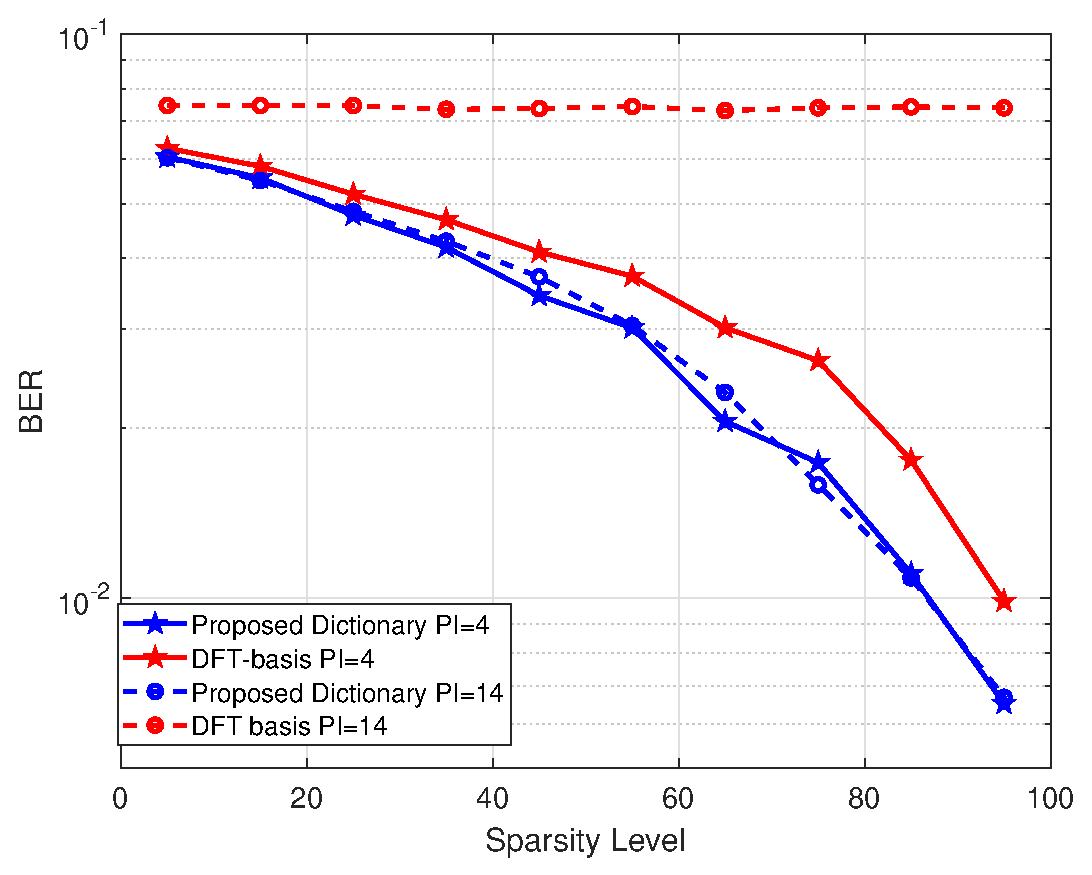
\includegraphics[width=110mm,height=80mm]{figures/figchap4/sparsity.eps}
	\caption{Analysis of DFT basis and \textcolor{black}{proposed} dictionary with different sparsity levels $s$ and pilot spacing for OMP algorithm}	
	\label{Fig_result1}
\end{figure}


Although there is a huge list of compressed sensing algorithms, having different benefits and drawbacks that are suitable for different systems/models, and with distinct convergence and complexity constraints, in the following figures we focus on some prominent greedy CS techniques, i. e., OMP, CoSaMP, IHT, NHTP \textcolor{black}{with dictionary,} compared to convex optimization based basic pursuit algorithms.

%\textcolor{blue}{Some greedy algorithms choose the elements that best approximate the signal at each iteration in a greedy fashion. While greedy thresholding algorithms choose such elements by fixing a threshold at each iteration and evaluating the elements that exceed such threshold in magnitude.}
%\textcolor{red}{We compare several compressed sensing algorithms with learned dictionary and DFT basis in order to find the best solution in terms of performance (BER) and complexity. CUT???} 

Fig. \ref{Fig_result2} illustrates the performance of CS algorithms with \textcolor{black}{the proposed dictionary}, showing that the basic pursuit method outperforms all the considered greedy algorithms in terms of BER, while the least square estimation (LSE) approach gives the worst performance. However, the curve of the greedy NHTP is really close the BP one, with the advantage of high computational complexity reduction.
Indeed, there is a trade-off between performance and computational complexity that we need to take into account, as shown in Sec. \ref{ComplexAnalysis}.
%\begin{figure}[ht]
%	\centering
%	\includegraphics[width=1\linewidth]{PI-4It-20Tx-100mod-32GI-16_iht.eps}
%	\caption{BER vs SNR for transmit antennas $N=100$, receive antenna $R=1$, number of channel taps $L_{taps}=6$}	
%	\label{Fig_result2}
%\end{figure}

\begin{figure}
	\centering
	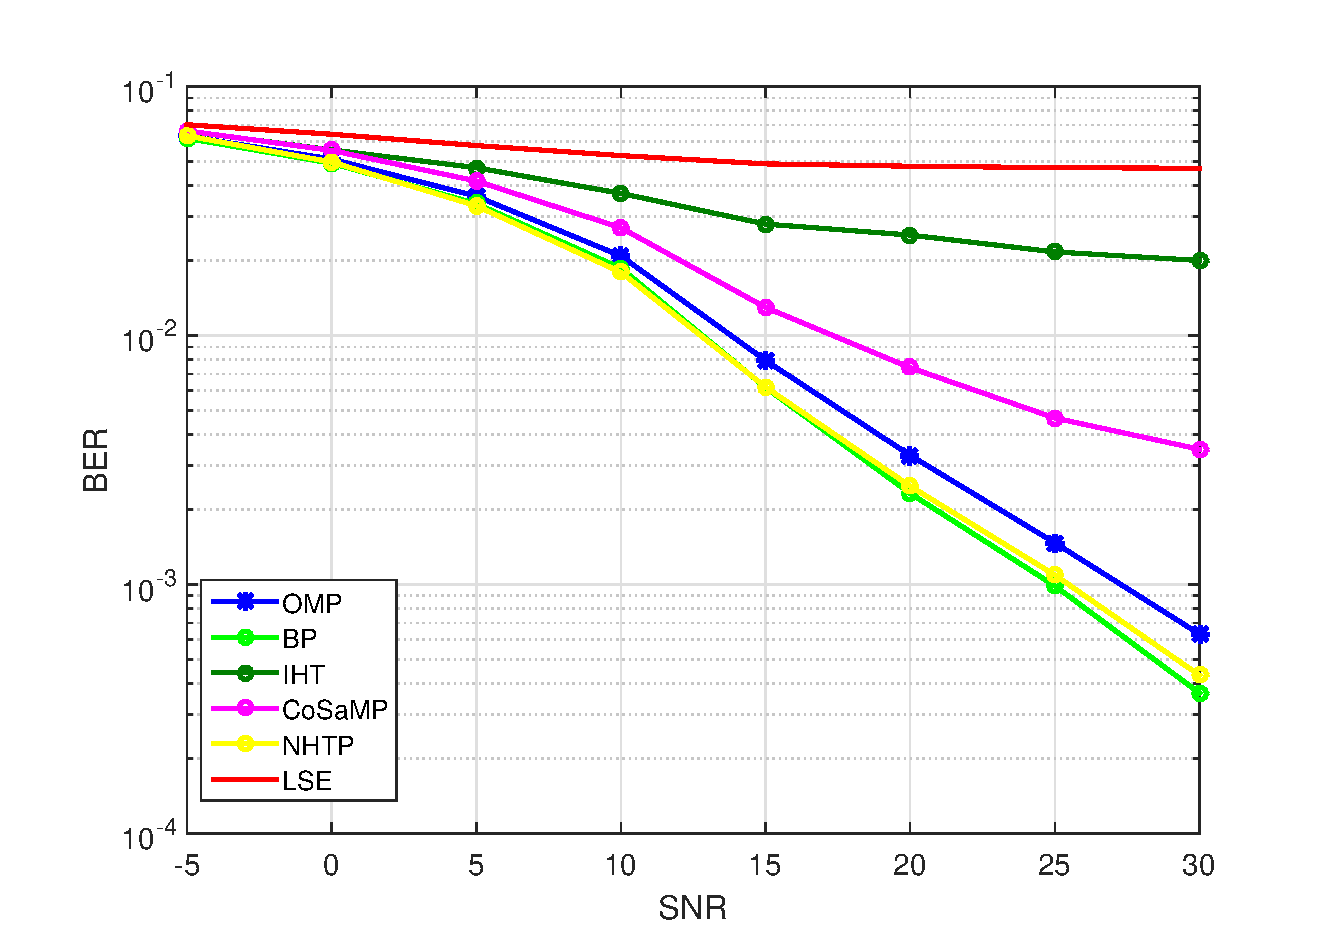
\includegraphics[width=120mm,height=85mm]{figures/figchap4/Fig2b.eps}
	\caption{Performance of CS techniques with \textcolor{black}{dictionary basis}: BER vs SNR (dB) for transmit antennas $N=100$, receive antenna $R=1$, number of channel taps $L_t=6$}	
	\label{Fig_result2}
\end{figure}

Finally, in Fig. \ref{Fig_result3} we analyze the effect of multipath channel for the NHTP \textcolor{black}{with the proposed dictionary} by varying the number of channel taps. We focus only on this algorithm since it is the best choice in terms of performance complexity trade off, as detailed in the following.

\begin{figure}
	\centering
	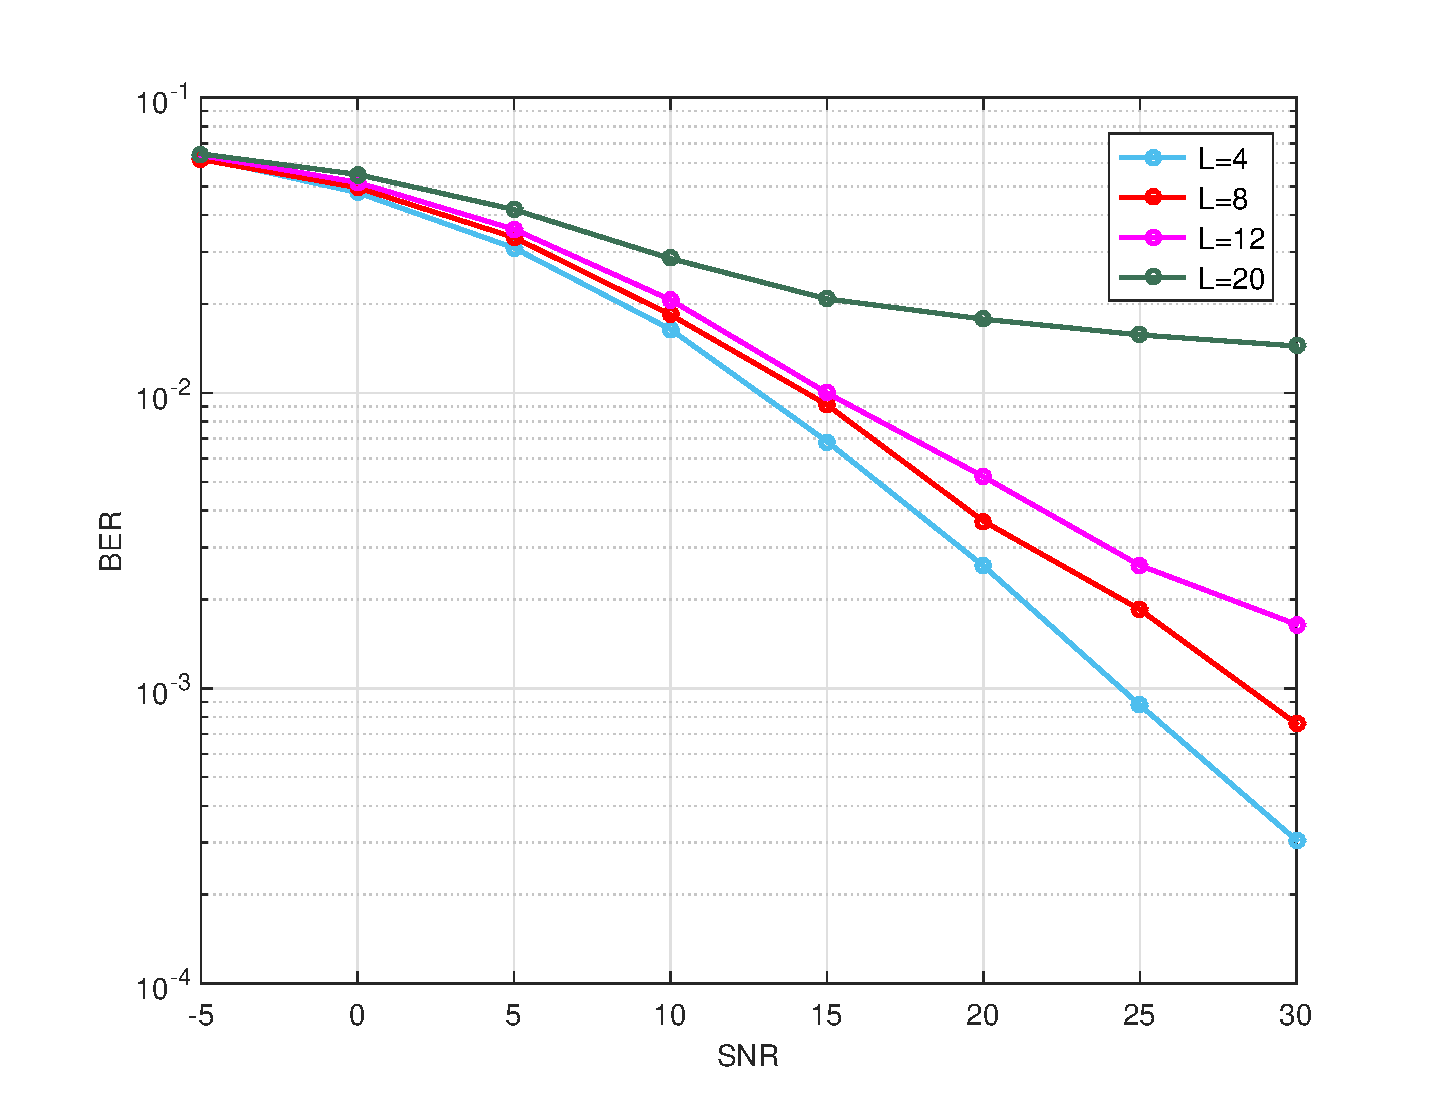
\includegraphics[width=120mm,height=85mm]{figures/figchap4/htp_L_1.eps}
	\caption{BER vs SNR (dB) for NHTP algorithm \textcolor{black}{with dictionary} changing the number of channel taps}	
	\label{Fig_result3}
\end{figure}
\textcolor{black}{
		Pilot overhead reduction has been compared among different compressed sensing based algorithms including convex optimization based BP and other greedy algorithms. It has been observed that the performance curve rapidly move down with decreasing pilot interval. The previous work \cite{pilot15} investigated pilot overhead reduction using CS based algorithm by random pilot allocation at different subcarriers for each antenna. They have used random sending matrix with DFT basis for sparse channel representation. In this section, we have assumed the same parameter setting for comparison purposes: transmit antennas = 128, number of subcarriers = 2048, SNR equal to 20 dB, $10$ percent pilots overhead, and MSE equal to -25 db. As shown in figure \ref{Fig_result7}, the proposed dictionary based algorithm exhibits better performance with pilot overhead less than $5$ percent at -30 db MSE.}
	\begin{figure}
		\centering
		\includegraphics[width=100mm,height=80mm]{figures/figchap4/pilot_over.eps}
     	%\includegraphics[width=1\linewidth]{pilot_over.eps}
		%\includegraphics[width=1\linewidth]{pilots.eps}
		\caption{Percentage pilot overhead}	
		\label{Fig_result7}
	\end{figure}
\subsection{Complexity Analysis}
\label{ComplexAnalysis}

\begin{table} \footnotesize
	\renewcommand{\arraystretch}{1.1}
	\caption{Computational complexity}
	\label{tabComplexity}
	\centering
	\begin{tabular}{cccccc}
		\textbf{BP}&\textbf{OMP}&\textbf{CoSaMP}&\textbf{IHT}&\textbf{NHTP}\\
		\hline
		\\
		O($n^3$)&O($s$ $m$ $n$)&O($m$ $n$)&O($m$ $n$)&O($m$ $n$)\\		
	\end{tabular}
\end{table}

\begin{figure}
	\centering
   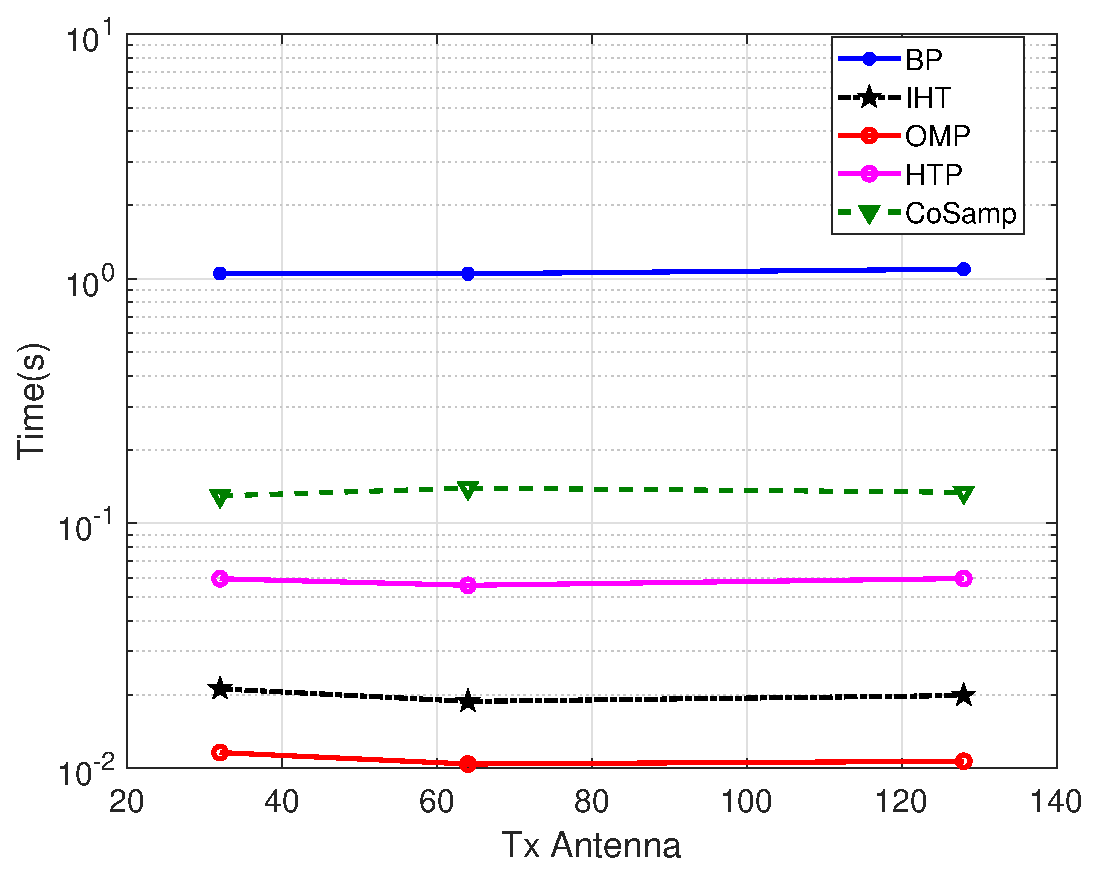
\includegraphics[width=100mm,height=75mm]{figures/figchap4/antennavstime_semilog.eps}
	\caption{Simulation time in seconds for CS techniques with \textcolor{black}{dictionary}}
	\label{FigComplex}      
\end{figure}



%\begin{figure}
%	\centering
%	\includegraphics[width=0.9\linewidth]{antennavstime_bp.eps}
%	\caption{Simulation time in seconds: BP and greedy algorithms}	
%	\label{FigComplex1}
%\end{figure}
%
%\begin{figure}
%	\centering
%	\includegraphics[width=0.9\linewidth]{antennavstime.eps}
%	\caption{Simulation time in seconds: greedy algorithms}	
%	\label{FigComplex2}
%\end{figure}

Tables \ref{tabComplexity} and Fig. \ref{FigComplex} refer to the computational complexity and the required simulation time, respectively.
%Note that \ref{FigComplex1} refers to simulation time for BP and greedy algorithms, while \ref{FigComplex2} only to the greedy algorithms to better illustrate the differences among them.

Considering Fig. \ref{Fig_result2}, \ref{FigComplex} and Table \ref{tabComplexity}, the greedy orthogonal matching pursuit and normalized hard thresholding pursuit show the best performance trade off in terms of BER and computational complexity/simulation time. Note that, although OMP shows the lowest simulation time in Fig. \ref{FigComplex}, the NHTP $BER$ performance in Fig. \ref{Fig_result2} greatly outperforms the OMP one, with a $2.5$ $dB$ gain at $10^-3$ $BER$. All the simulations are performed on an intel core i5 (7th Generation) architecture.

\section{CONCLUSION}
\label{Concl}
We have proposed a CS based channel estimation \textcolor{black}{with a suitable dictionary} for downlink beamforming in massive MIMO-OFDM FDD systems. We have exploited CS techniques to reduce training overhead, that is proportional to the sparsity level of the channel. The sparse channel representation is obtained through a \textcolor{black}{proposed dictionary} able to self-adapt to the cell characteristics. 
We have analyzed several CS algorithms in order to select among them the best technique with respect to the \textcolor{black}{proposed dictionary}. Numerical results demonstrate that basic pursuit shows the best performance at the cost of a higher complexity, while greedy solutions give good results with a lower complexity and hence shorter training period. Among them, the NHTP approach is the greedy algorithm with the best performance complexity trade-off.


%%%%%%%%%%%%%%%%
 %Chapter 5
%%%%%%%%%%%%%%%%

%\chapter{Joint Channel Recovery from Quantized feedback}
Accurate channel state information (CSI) at the transmitter is an essential prerequisite for transmit beamforming in massive multiple input multiple output (MIMO) systems. However, due to a large number of antennas in massive MIMO systems, the pilot training and feedback overhead become a bottleneck. To resolve this issue, the research work presents a novel framework for frequency division duplex (FDD) based multi-user massive MIMO systems. In the given framework a 2-step quantization technique is employed at the user equipment (UE) and the CSI is recovered at the base station (BS) by applying the proposed compressed sensing (CS) based algorithm. In further detail, the received compressed pilots are quantized by preserving 1 bit per dimension direction information as well as the partial amplitude information. Subsequently, this information is fed back to the BS, where the BS employs the proposed partially joint orthogonal matching pursuit (Q-PJOMP)/ quantized partially joint iterative hard thresholding (Q-PJIHT) CS algorithms to recover the CSI from this limited and quantized feedback. The presented CS algorithm utilizes the appropriate dictionary and also exploit the hidden joint sparsity structure among users to jointly estimate the channel, resulting in the reduction of the information feedback required for CSI estimation. Simulations are performed using SVD and MMSE beamforming utilizing estimated channel and results confirm that the proposed 2-step quantization approaches the system with channel knowledge without quantization. Moreover, the proposed 2-step quantization outperforms  1-bit quantization. In other words, the proposed system overcomes the training overhead problem, on top of that the feedback bits are also reduced without significantly compromising the performance.
\section{Introduction}
\label{sec:intro}
Massive multiple input multiple output (MIMO) is one of the emerging technology in wireless communication. It employs a large number of transmit antennas at the base station (BS), which makes the system more reliable and enhances the throughput as compared to traditional MIMO \cite{mimo-gain}. The high throughput is achieved by improving spectral efficiency, mitigating inter-user interference and employing more directional beams \cite{mimo-gain}. The massive MIMO system can serve various users simultaneously in the same time-frequency block, due to the large deployment of antennas at the BS. Nevertheless, serving many users concurrently is challenging due to the interference among them. The interference problem among users can be mitigated if each user has its aligned beam, which is obtained with appropriate precoding/beamforming techniques at BS. However, the accurate beamforming requires proper channel state information (CSI) at the transmitter. Traditionally, CSI can be obtained by using time division duplex (TDD) or frequency division duplex (FDD) schemes.\\ 
In TDD, both uplink (UL) and downlink (DL) operate at the same frequency bands, but in separate time slots. A channel estimate in one band can be utilized in the other, thanks to channel reciprocity. Consequently, in TDD if the channel estimate is obtained in UL, by employing the channel reciprocity, this estimate is also applicable to DL.  The primary constraint of TDD is that acquisition and utilization of CSI  should be performed within the coherence time \cite{mimo_eric2}. Therefore, users have to transmit their pilots simultaneously within this coherence time. Since the pilots should be orthogonal to evade interference among them, the limited number of available orthogonal sequences may result in pilot contamination \cite{mimo_eric2}.\\
Unlike TDD, in FDD the channel reciprocity is no longer applicable since UL  and  DL  are in separate bands. Despite the advantage of channel reciprocity in TDD, FDD is important in two ways; firstly, it is considered more robust to delay-sensitive applications \cite{FDD_or_TDD},  secondly, most of the existing systems are already deployed in FDD.  Therefore, it is of great significance to improve and enhance the approaches to obtain CSI in FDD systems.
Since channel reciprocity can not be exploited in FDD, DL and UL channels are separately estimated. Typically, the training is done in DL by estimating CSI at the users, this CSI is sent to the BS in the uplink using a dedicated signaling link. However, the number of pilots required for training grows linearly with the number of transmit antennas at the BS. Since massive MIMO have a large number of BS antennas, the pilot training and feedback overhead have become the bottle-neck in FDD \cite{Dict_learning}.

One of the potential solutions to resolve the training overhead problem is to explore an appropriate technique for reducing feedback overhead.
The research work in \cite{sparse_channel} and the experimental studies in \cite{exp-vitual} reveal that the increase in the number of BS antennas results in limited prominent transmission directions per user.  Since there are few scatters at the BS side as compared to the number of antennas, the channel matrix will tend to be sparse \cite{mainref-joint,exp-vitual}. 
In this scenario, to estimate the channel, compressed sensing (CS) paradigm can be utilized to represent a high dimensional channel vector into low dimension \cite{ourwork,Dict_learning,sparse_channel}. The main objective of the aforementioned research works is to reduce the number of pilot training overhead by taking advantage of the channel sparsity in general, without exploiting any structure in the measurements. Besides the channel sparsity, it has been observed that the users are mostly located in the vicinity sharing common scatters, for example, in offices, playgrounds, streets, apartments. Due to these scatters, the channel is strongly correlated between the multi-antennas of each user, known as  "intra-user joint channel sparsity", and among closely located distinct users,  termed as "inter-user joint channel sparsity"  \cite{book_enrico}. \\
The research works in \cite{usr_grp,beamblock}, exploit inter-user joint sparsity to estimate the channel. The central idea is based on grouping users with common channel statistics, which will decrease the pilot overhead \cite{usr_grp}. Subsequently, the inter-user joint sparsity can be applied within each of these groups. The research work \cite{beamblock} utilizes the beam-block sparsity model to compress the pilots in DL, which are then fed back to UL in a quantized form and applied at BS to obtain CSI through CS.
However, \cite{usr_grp,beamblock} do not consider intra-user or partial joint user sparsity. Other notable research works \cite{distributed_cs, JSM} laid the theoretical foundations for modeling intra and inter-user joint sparsity, known as joint sparsity model (JSM).  Utilizing the ideas of JSM, a class of algorithms under the paradigm of distributed compressed sensing (DCS) exploits Intra and the inter-channel correlation between users to unveil joint sparsity structure in the massive MIMO system \cite{mimo-common-sparsity, mainref-joint,mainref-1bit,distributed_def}. 
Although the research work in \cite{mainref-joint} \cite{ourwork} \cite{beamblock} substantially reduced the training overhead problem, the feedback pilot bits are still considerably high.  Thus, besides reducing the number of measurements, some work has also been done to lower the number of feedback bits using direct quantization \cite{Limited_feedback,limited-feedback_RWheath}. However, this type of direct quantization is complex and requires several bits per symbol for decoding to achieve better performance. Another extreme case of feedback reduction is 1-bit per dimension using CS algorithms as discussed in \cite{mainref-1bit}. However, it hardly provides directional information and power information is lost in this manner.  The power control information is very critical for CSI since it captures the effect of scatters, multipath fading and signal strength deterioration with distance. To improve the performance, \cite{beamblock} presents a scheme to quantize both the amplitude and phase of the received pilots, thus preserving both directional and power information, at the expense of considerably increased feedback overhead.

The presented work is inspired by \cite{beamblock} in terms of considering both amplitude and phase information. However, we have observed that it is more efficient to quantize the complex pilot phase information with 1-bit per dimension as in  \cite{mainref-1bit} and acquire partial amplitude information by averaging the amplitude of compressed received pilots.  Therefore, the phase information in 1-bit compressed form as  \cite{mainref-1bit} along with the amplitude information is sent back to the BS using a more simplified  technique than \cite{beamblock} In contrary to \cite{beamblock} that uses eigenbeam model (EBM),  our work is based on virtual channel model (VCM), which uses Fourier basis instead of eigenbasis \cite{exp-vitual}. Although VCM and EBM models are comparable in terms of system capacity and performance, VCM is inherently less complex, is more suitable for uniform linear arrays (ULAs) and can be readily extendable to frequency-selective channel \cite{exp-vitual}.
This research work presents a quantized feedback-based algorithm for partially joint channel estimation in massive MIMO systems. It preserves both power control information as well as directional information in an efficient and simplified manner. To achieve this goal the pilots are transmitted from BS to each user equipment (UE), subsequently, these received pilots are quantized using a two-step quantization method.  Eventually, the quantized information is fed back to BS, the BS uses the proposed CS-based recovery algorithms: quantized partially joint orthogonal matching pursuit (Q-PJOMP) or quantized partially joint iterative hard thresholding (Q-PJIHT), to recover the channel from the quantized feedback. This recovered channel information is utilized by the transmit beamforming to reduce inter-user interference. Our work uses realistic imperfect channel information as opposed to \cite{mainref-joint,mainref-1bit} that assume perfect channel knowledge to perform beamforming.
Besides presenting efficient feedback techniques and better channel estimation algorithms; two types of transmit beamforming namely: (i) minimum mean square error (MMSE) or regularized zero-forcing (RZF), and (ii) singular value decomposition (SVD), are employed with realistic estimated imperfect channel information. Effectively, we have focused on multiple aspects of communication and presented a complete system for CSI acquisition spanning all three main stages: (i) channel estimation, (ii) beamforming procedure, (iii) data detection. 

The main contributions of this work are as follows:

\begin{itemize}
    \item This research work presents two novel distributed CS-based algorithms; Q-PJOMP and Q-PJIHT, to estimate a partially joint channel by utilizing quantized feedback in massive MIMO systems. The feedback bits are reduced without compromising significant performance gain while preserving power and directional information, as compared to \cite{mainref-1bit} that considers only directional information. 
    \item An efficient dictionary-based sparsifying matrix has been adopted, which is more effective as compared to the square DFT based sparsifying matrix especially for the frequency selective channel.
     \item Besides improved channel estimation algorithms, two precoding techniques, namely MMSE and SVD, are applied for efficient transmit power and reduced inter-user interference.
    \item A realistic CSI estimate is acquired and utilized in the transmit beamforming procedure, as compared to the common perfect channel knowledge assumption as in  \cite{mainref-joint,mainref-1bit}. Furthermore, we have investigated a more realistic frequency selective channel, instead of a flat fading as in \cite{mainref-joint,mainref-1bit}. \end{itemize}

Simulation results reflect that Q-PJOMP is the most suitable algorithm to estimate the partially joint channel from quantized feedback. Moreover,  by applying MMSE based transmit beamforming, the system performance is significantly improved.  The remainder of the paper is organized as follows. Sec.
II describes the massive MIMO OFDM based system model,
 particularly the spatial correlations of users' channels are emphasized with limited feedback per dimension. Sec. III addresses the proposed CS techniques for training and feedback schemes, i. e. Q-PJOPM and Q-PJIHT, exploiting the distributed joint channel sparsity model. Sec. IV presents the simulation results for performance evaluation, finally, conclusions are drawn in Sec. V.


\section{System Model}
\label{sec:sysmodel}
\subsection{Massive MIMO OFDM System}
 Consider a single-cell multi-user massive MIMO OFDM transmission over a quasi-static frequency selective fading channel. The system is composed of a base station (BS) and K users in FDD mode. The number of antennas at BS is equal to $N_t$ and each user is equipped with $N_r$ antennas, where $N_t$ is very large.  The over all system model can be represented as follows: 
\begin{equation}
\mathbf{Y}_{i} = \mathbf{H}_i \mathbf{X}_i + \mathbf{N}_i
\label{eq_channel}
\end{equation}
Where $\mathbf{X}_i  \in \mathbb{C}^{N_t \times T}$ is the transmitted signal in $T$ time slots, $ \mathbf{H}_i \in \mathbb{C}^{N_r \times N_t}$ is the channel matrix from the BS to the $i^{th}$ user, $\mathbf{N}_i  \in \mathbb{C}^{N_r \times T}$ is the Gaussian  noise, and $\mathbf{Y}_{i} \in \mathbb{C}^{N_r \times T}$ is the received signal on each $i^{th}$ user.  
The fading channel between each transmit antenna and $i^{th}$ user is considered as frequency-selective and has $L$ uncorrelated channel taps. For $N_r \times N_t$ MIMO channel, the frequency response can be written as:
\begin{equation}
     \mathbf{H}_i(f)= \sum_{l=1}^L \mathbf{\beta}_l \mathbf{a}_r(\theta_{r,l}) \mathbf{a}_t(\theta_{t,l}) e^{-j2\pi f \tau_l}
\end{equation}

\begin{figure*}
\centering
\includegraphics[scale=0.37]{figures/fig_ch_rec/joint_channelplus_cir.jpg}
\caption{System description of downlink (solid) and feedback link (dotted) for joint channel sparsity with local scatters (LSc) and common scatters (CSc), Channel impulse response is also given for all three users.}
\label{sys_fig}
\end{figure*}
Where $\mathbf{\beta}_l$ is the complex amplitude for $l^{th}$ path, $\tau_l$ is the  $l^{th}$  path delay, $\theta_{r,l}$ and $\theta_{t,l}$ are the transmitted and received path angles and $\mathbf{a}_r$, $\mathbf{a}_t$ represents array steering and response vectors of transmitted/received signal in the direction of $\theta_t$/$\theta_r$. To mitigate frequency selective fading the OFDM scheme is used \cite{reviwsparse,CRRM2011,Vizziello2013}. An OFDM symbol duration $T_{sym}=(N_o+G)\cdot T_s$ is considered, where $N_o$ is the number of subcarriers equally spaced in frequency at ${\Delta} f=\dfrac{1}{T_s}$, with the sampling time $T_s$, and $G$ is the guard interval in number of samples, which is set larger than the expected channel delay spread to further reduce the inter-symbol interference (ISI) \cite{reviwsparse}. 
\label{formulation}
\subsection{Distributed Joint Channel Sparsity Model}
\label{lbDis_JCS}
In any particular cell, there are some dominant scattering clusters whose position is determined from the specific attributes of the cell itself, like the presence of buildings or other propagation obstacles. These scatters can be shared by users regardless of their position \cite{Dict_learning}.  Massive MIMO experiments \cite{exp-vitual} prove that channel matrices at the user side is sparse due to the limited local scatters at the BS \cite{mimo-common-sparsity}, and maybe jointly correlated
due to the shared common local scattering clusters \cite{corr_pathdelay}. Thus, both per-link and joint channel sparsity can be exploited through CS-based solutions to reduce training and feedback overheads.
The inter-user channel sparsity can be further explained based on how scatters are shared among users: 
\begin{itemize}
  \item The scatters shared among all users are known as common scatters (CSc), for example, in Fig. \ref{sys_fig} CSc are shared among all UE, these common scatters will produce \textit{joint sparsity}.
  \item The scatters for a single user or shared among the subgroup of users is known as local scatters (LSc). For example, in Fig. \ref{sys_fig} LSc1, LSc2, and LSc3 are local scatters for UE1, UE2, and UE3 respectively, while, LSc1 and LSc2 are shared among UE1 and UE2. In the case of LSc, the inter-user joint sparsity will be limited to a sub-group of users sharing the LSc, this is termed as \textit{partial joint sparsity}. 
\end{itemize}

The presented research work considers a uniform linear array (ULA) model for both BS and user side antennas. To represent spatio correlation channel for ULA in angular domain, the virtual channel representation can be considered. The experimental studies in \cite{exp-vitual} confirms that spatial channel can be transformed into angular domain as follows:

\begin{equation}
\mathbf{H}_i^a=\mathbf{F}_{R_i}^H \mathbf{{H}}_i \mathbf{F}_{T_i} \text{,}\quad \quad \mathbf{H}_i=\mathbf{F}_{R_i} \mathbf{{H}}_i^a \mathbf{F}_{T_i}^H
\label{eq-VCM}
\end{equation}

 Where $\mathbf{F}_{R_i}\in \mathbb{C}^{N_r\times N_r}$ and $\mathbf{F}_{T_i}\in \mathbb{C}^{N_t\times N_t}$ represent the unitary  matrices with Fourier basis. This transforms the channel at BS and user side from a spatial domain to the virtual angle domain.
$\mathbf{H}_i^a \in \mathbb{C}^{N_r\times N_t}$ is the virtual channel representation and can be considered equivalent to the actual spatial channel $\mathbf{{H}}_i$ in Fourier domain \cite{exp-vitual}. The non-zero $(c,d)$-th entry of $\mathbf{{H}}_i^a $ indicates the spatial path from the $c$-th BS transmit direction to $d$-th receive direction of the $i^{th}$ user.
 Equation (\ref{eq-VCM}) has been used to represent the spatial channel in the angular domain with the sparsifying matrix F  \cite{mainref-joint,Dict_learning}. Although with angular domain representation channel sparsity is guaranteed, however, to obtain it explicitly for per link and joint channel sparsity, the design of sparsifying matrix $\mathbf{F}$ is very critical. In \cite{mainref-joint} and \cite{mainref-1bit} a sparsifying matrix $\mathbf{F}$ is considered as square DFT matrix, but in \cite{Dict_learning} and \cite{ourwork} it has been shown that by introducing more redundancy in sparsifying matrix $\mathbf{F}$ improved channel representation can be achieved, further details are discussed in section \ref{sec:dict_formation}.  
Fig. \ref{sys_fig} shows the system description with local and common scatters in a multi-user MIMO system. The left-hand side of the figure explains the joint sparsity structure by displaying varying support indexes (non-zeros entries) in different colors in the channel matrix. For example, the scatters shared among all users are represented by the common support $\Theta_c$ indicated in red, the support of the scatter shared only by some users is shown in green, and of the local scatters is represented in blue. The individual support $\Theta_i$ represents the non-zeros entries of each user. The left-hand side shows the position of the support, while the right-hand side shows that there will be different values for these supports. Besides, the right-hand side also gives a snapshot of the channel delay profile for different users in this hypothetically generated propagation environment.

The sparsity of the massive MIMO channel may be explained as follows \cite{mainref-joint,mainref-1bit,book_enrico}: 

\begin{enumerate}
\item \textbf{Intra-User Joint Sparsity (Individual joint Sparsity):}\\
Since there are more than one receiver antennas $N_r$  per user, the channel will exhibit intra-user joint sparsity. This effectively means that there will be channel dependency among different antennas of each user at the same time. This dependency is produced by local scatters.  Consequently, the receiver channel matrix elements will be extremely correlated and its row vectors will usually have the same sparsity support. Specifically, the matrix $\mathbf{H}_i^a$ is a row sparse and for each user $i$, the $j^{th}$ row vector $\mathbf{H}_i^a(j)$ will have same support $\Theta_i$ such that $0<|\Theta_i|\ll N_t$, i.e.,
\begin{equation}
    \Theta_{i1}=\Theta_{i2}=\hdots =\Theta_{iN_r}
    \simeq\Theta_i
\end{equation}
\item \textbf{Inter-User Sparsity (Distributed Joint Sparsity):}
Inter-user sparsity exploits the channel dependency among different users at the same time\cite{book_enrico}. It refers to the scenario of a massive MIMO system where different users are close enough to share some common scatter. Therefore, the channel matrices of different users will be highly correlated and will have common sparsity support $\Theta_c$:
\begin{equation}
    \Theta_c= \bigcap_{i=1}^{K} \Theta_i
\end{equation}

This common sparse support will be a subset of individual sparse support if users are sharing some common scatters, such that $\Theta_c \subseteq \Theta_i$. However, if there are only common scatters among users, then the individual sparsity support will be equal to the common sparsity support.
There is the possibility that none of the users are sharing any common scatter, in that case, $\Theta_c=\emptyset$  \cite{mainref-joint}.
\end{enumerate}

\subsection {\textbf{Limited feedback based channel recovery and beamforming}}
\label{LF_framework} 
\begin{figure*}[h!]
    \centering
    \includegraphics[scale=0.44]{figures/fig_ch_rec/flow_chart_MIMO.jpg}
   \caption{Flow chart of the complete procedure of CSI acquisition and utilization. }
    \label{fig:CSI_flow}
\end{figure*}

The current section discusses the overall procedure for channel recovery from the quantized feedback pilots and utilization of that estimate for transmit beamforming as shown in Fig. \ref{fig:CSI_flow}. The BS sends pilots in the DL, which are quantized at each UE and are fed back to BS via a dedicated uplink signaling channel. The BS utilizes these quantized pilots to exploit channel's hidden joint sparsity for channel estimation using distributed CS algorithms. Eventually, the recovered channel is employed for beamforming at the transmitter for more reliable data detection at the receiver. Each step is further explained as follows:  

 
$\bigstar$ \textbf{Step-1 Downlink training:}  
As discussed in Sec. \ref{sec:intro}, to obtain CSI of the DL at the transmitter in FDD, the pilots are sent in DL. For this purpose, the BS broadcasts $T$ common training symbols to the $K$ users over the downlink. Therefore, the received pilots for the $i^{th}$ user can be written as:
\begin{equation}
\mathbf{Y}_{pi} = \mathbf{H}_i \mathbf{X}_p + \mathbf{N}_i
\label{eq_channel_pilot}
\end{equation}
Where $\mathbf{X}_p  \in \mathbb{C}^{N_t \times T}$ is the concatenated transmitted pilots, and $\mathbf{Y}_{pi} \in \mathbb{C}^{N_r \times T}$ is the received pilots on each $i^{th}$ user as shown in step-1 of Fig. \ref{fig:CSI_flow}. \\
   
   
$\bigstar$ \textbf{Step-2 Quantization:}
The received pilots $\mathbf{Y}_{pi}$ are quantized at each UE to reduce the number of feedback bits, as shown in step-2 of Fig. \ref{fig:CSI_flow}. It is represented as $Q(\mathbf{Y}_{pi}$), however, the quantization process may also induces some error as follows: 
\begin{equation}
\mathbf{\hat{Y}}_{pi} =Q(\mathbf{Y}_{pi})+ \mathbf{\Gamma}_i
 = Q(\mathbf{H}_i \mathbf{X}_p + \mathbf{N}_i) + \mathbf{\Gamma}_i
\label{eq_qunatization}
\end{equation}
Where Q(.) is the uniform quantization function that maps the complex pilots to bits [+1, -1] and $\mathbf{\Gamma}_i$ is the quantization error. In the presented work, pilots are quantized by preserving both direction and amplitude, as opposed to \cite{mainref-1bit}, where pilots are quantized to the extreme 1-bit case. The 1-bit scheme lacks power information, having only directional information, this results in poor channel estimate. Therefore, we have considered averaged quantized amplitudes of the received pilot for each user. The averaged amplitude  $\mu_i=\frac{1}{P_t} \sum_i^{P_t} |\mathbf{Y}_{pi}|$ of the received complex pilot $\mathbf{Y}_{pi}$ is determined for each user.  Subsequently, these averaged amplitudes are quantized to 2 bits per user.  Furthermore, the direction information is  computed using 1 bit per dimension from the received pilots, given as:

\begin{equation}
\mathbf{Y}_{pi}=\text{sign(Re}(\mathbf{Y}_{pi}))+j\text{sign(Im}(\mathbf{Y}_{pi})) 
\label{eq_qunatization}
\end{equation}

The amplitude information $\mu$ is fed back along with the direction information to the BS,  this is further described in algorithm \ref{algo1}. \\
  
 
$\bigstar$ \textbf{Step-3 Channel recovery using CS:}
The quantized pilots determined in step 2 are fed back to BS in UL. At the BS, CS-based algorithms are applied to recover the channel. The BS employs the 2-bit partial amplitude information per users along with 1 bit per dimension direction information of each user to recover the channel jointly for all users. It is important to mention that as the users are sharing the channel, therefore, partial amplitude along with direction information is sufficient to jointly estimate the partially correlated channel. For this purpose, the CS-based JOMP \cite{mainref-joint} and BIHT algorithms \cite{mainref-1bit} are modified. This facilitates channel recovery using quantized feedback information.  We have proposed two novel distributed CS-based greedy algorithms for better analysis in terms of complexity and performance, The Q-PJIHT  \ref{algo2} and Q-PJOMP are given in algorithm \ref{algo3}, respectively. 

Further details of CS-based channel recovery and proposed CS algorithm is provided in section \ref{sec:dict_formation}. \\

$\bigstar$ \textbf{Step-4 Beamforming:}
During step 3 estimate of the channel, $\mathbf{\hat{H}}_i$  becomes available at the BS side, it is employed to achieve transmit beamforming, as shown in step 4 of Fig. \ref{fig:CSI_flow}. The precoding matrix is constructed by applying this estimate, it overcomes the inter-user interference and decorrelates users in a highly correlated environment. Furthermore, the precoding matrix is beneficial for data detection to decorrelate users. In particular, we have focused on minimum mean square error (MMSE) or regularized zero-forcing (RZF), as shown in equation (\ref{eqMMSE}). It attempts to maintain strong signal gain while limiting interference among users.  MMSE based precoding is more reliable than ZF, since ZF amplifies the noise in the presence of highly correlated user channel. Moreover, MMSE precoder is not only robust for MU-MIMO systems where users are located in the vicinity, but it also provides stable performance at high SNRs\cite{precding_survay}.  MMSE precoder is considered as the more suitable choice for linear precoding in MIMO based wireless systems \cite{precding_survay,precoding_emil}. For MMSE based precoding, the received signal model in equation (\ref{eq_channel}) is revisited  by including the beamforming matrix $\mathbf{W}$  as follows: 
\begin{equation}
\text{MMSE}
\begin{cases}
%\mathbf{{Y}}_{pi}=Q(\mathbf{Y}_{pi})\\
\mathbf{G}= \mathbf{\hat{H}}^H (\mathbf{\hat{H}} \mathbf{\hat{H}}^H +\lambda \mathbf{I} )^{-1 } \\
\eta= \sqrt{\frac{N_t}{Tr (\mathbf{G} \mathbf{ G}^H)}}\\
\mathbf{W}= \eta \mathbf{G} \\
\mathbf{Y}_i=\mathbf{X}_i \mathbf{W}_i \mathbf{H}_i +\mathbf{N}_i\\
%\mathbf{Y}_{pi}=Q(\mathbf{X}_p \mathbf{W}_i \mathbf{H}_i +\mathbf{N}_i) 
\end{cases}
\label{eqMMSE}
\end{equation}
 In the above equation, $\lambda= N_t \sigma^2 /K$ is the regularization factor, if $\lambda=0$, the MMSE precoder becomes equal to a ZF. The MMSE optimal precoder $\mathbf{G}$ is obtained from the estimated channel $\mathbf{\Hat{H}}$ of all users.
In the next step $\mathbf{G}$ is scaled with the power scaling factor $\eta$ to minimize the mean square error (MSE) under the  BS transmit power constraints \cite{power_MMSE}. Primarily, $\eta $ is used for power allocation at the BS to minimize the total power consumption under some given noise and interference related constraints. While $\lambda$ attempts to maintain the strong signal gain with limited interference among users.
Besides the MMSE precoder in equation (\ref{eqMMSE}), for comparison purpose an SVD based beamforming is also applied, as shown in equation (\ref{eqsvd}) . It can be noted that we do not assume perfect channel knowledge. Accordingly, the estimate of realistic channel can be decomposed using SVD, and is given as follows:  
\begin{equation}
 \mathbf{\hat{H}}_i=\mathbf{\hat{U}}_i \mathbf{\hat{\Lambda}}_i \mathbf{\hat{V}}_i^H
\label{eq-svd}
\end{equation}
Where $\mathbf{\hat{U}}_i\in \mathbb{C}^{N_r\times N_r}$ and $\mathbf{\hat{V}}_i\in \mathbb{C}^{N_t\times N_t}$ represent the unitary  matrices, such that $\mathbf{\hat{V}}_i^H\mathbf{\hat{V}}_i=\mathbf{\hat{U}}_i\mathbf{\hat{U}}_i^H = \mathbf{I}$ and
$\mathbf{\hat{\Lambda}}_i\in \mathbb{C}^{N_r\times N_t}$ is a diagonal matrix. But, as we have considered realistic channel $\mathbf{\hat{H}}_i$,  therefore, the estimated channel characteristics will not exactly match with that of the ideal channel. Consequently, the unitary property $\mathbf{{V}}_i^H\mathbf{\hat{V}}_i = \mathbf{I}$ does not hold any more and this may induce interference.  Nevertheless, these ramifications can be combatted provided the channel estimate is robust. Based on SVD decomposition, the equation (\ref{eq_channel}) is revised and beamforming equations can be given as: 
\begin{equation}
\text{SVD}
\begin{cases}
\mathbf{\hat{X}}_i= \mathbf{\hat{V}}_i^H  \mathbf{X}_i    \\
\mathbf{{Y}}_i=\mathbf{H}_i \mathbf{X}_i+\mathbf{N}_i=(\mathbf{U}_i \mathbf{\Lambda}_i \mathbf{V}_i^H)  \mathbf{X}_i+\mathbf{N}_i , \,\,\,\,\,\,\,\,\,\, \forall_i \in K\\
\mathbf{\hat{U}}_i^H\mathbf{{Y}}_i=\mathbf{\hat{U}}_i^H (\mathbf{U}_i \mathbf{\Lambda}_i \mathbf{V}_i^H)   \mathbf{\hat{V}}_i \mathbf{\hat{X}}_i+\mathbf{\hat{U}}_i^H\mathbf{N}_i, \,\,\,\,\,\,\,\,\,\, \forall_i \in K\\
\mathbf{\hat{Y}}_i= \mathbf{\Lambda}_i \mathbf{\hat{X}}_i+\mathbf{\hat{N}}_i
\end{cases}
\label{eqsvd}
\end{equation}
Where $\mathbf{\hat{X}}_i$ is the precoded signal at the transmitter, $\mathbf{\hat{N}}_i= \mathbf{\hat{U}}_i^H\mathbf{N}_i$ is the noise term, and $\mathbf{\hat{Y}}_i =\mathbf{\hat{U}}_i^H\mathbf{{Y}}_i$ is the decoder for the transmit beamformer at the receiver side. 

\begin{algorithm}[H]
\SetAlgoLined
 \textbf{Step-1:} A common training pilot vector $\mathbf{X}_p$ is transmitted from BS to all the users.\\ 
 \textbf{Step-2:} Each user's received pilots are quantized using two steps:
 \begin{enumerate}
     \item[(a)]  The averaged amplitude $\mu_i$ of the received  pilot vector $\mathbf{Y}_{pi}$ is calculated for each user. Then these averaged amplitudes are quantized to 2 bits per user;
     \item[(b)] the sign information is achieved with 1 bit per dimension from the received pilots:\\ $S(\mathbf{Y}_{pi})=S(\mathbf{H}_i\mathbf{X}_{p}) $ such that\\ $S(\mathbf{Y}_{pi})=\text{sign(Re}(\mathbf{Y}_{pi}))+j\text{sign(Im}(\mathbf{Y}_{pi}))$ .
 \end{enumerate}
 \textbf{Step-3:} Each user feedbacks the obtained quantized and reduced $\mathbf{Y_{pi}}$  to BS.\\
\textbf{Step-4:} The channel is jointly recovered for all users from the quantized feedback pilots $\mathbf{Y}_{pi}$ using distributed CS at BS.\\
\caption{Joint channel recovery framework from quantized feedback}
 \label{algo1}
\end{algorithm}
 
\section{Compressive Channel estimation with limited feedback}
\label{sec:dict_formation}
In sec. \ref{LF_framework}, the overall framework has been described, it consists of channel estimation, beamforming matrix design, and data detection. The channel estimation is performed at the BS side using the quantized pilots received on UL from UE, as indicated in step-3 of Fig. \ref{fig:CSI_flow}.  The current section will discuss compressed sensing algorithms and dictionary design in more detail. 

\subsection{Comparison of dictionary and DFT basis for measurement matrix design}
A channel that exhibits only a few dominant propagation paths may be considered sparse and is approximated as a linear combination over a known basis or dictionary, resulting in a sparse channel response \cite{reviwsparse}.  Conventionally, DFT basis $\phi$ have been utilized for sparse channel representation \cite{reviwsparse,beamblock,dft,mainref-joint,mainref-1bit} as shown below.  
    \[
 \mathbf{    \phi= \frac{1}{\sqrt{N_t}}
    \begin{bmatrix}
e^{-j2\pi k_{1,1}} &\dots& e^{-j2\pi k_{1,N_t}} \\
e^{-j2\pi k_{2,1}} &\dots& e^{-j2\pi k_{2,N_t}} \\
\vdots & \ddots & \\                                          
e^{-j2\pi k_{N_t,1}}  &\dots& e^{-j2\pi k_{N_t,N_t}} \\
    \end{bmatrix}}
    \]    \\
The usage of the DFT basis is compliant with the theoretical results of signal estimation in CS\cite{Candes08}, therefore, the DFT basis are employed in sparse channel representation. Considering normalized DFT basis $\phi$ as a sparsifying matrix, the sparse channel response can be written as, $\mathbf{\hat{H}}_i=\phi \mathbf{B}_{si}$, where $\mathbf{B}_{si} \in \mathbf{C}^{N_t \times N_r}$ is the sparse matrix. As described earlier in equation (\ref{eq-VCM}), such modeling is applied to represent spatial channel response into the angular domain, also known as the virtual channel model. Though, the DFT basis represents the channel only in a few directions. In a real-world scenario, the actual signal can emanate from arbitrary directions, which may differ from the one represented in the DFT matrix. This results in leakage effect and poor channel estimate.  In case the channel is highly correlated or exhibits multipath, the leakage effect worsens even further \cite{Dict_learning}. 

To estimate the channel accurately, a robust and effective basis is an essential prerequisite. To construct an improved and substantial basis or dictionary, we extended the squared DFT matrix by proposing added redundancy and considering the channel delay profile as in \cite{ourwork}. The objective is to build a more flexible and enhanced representation of the channel. In the dictionary formulation, the channel delay profile $\tau_{ch}$ can be represented using OFDM sample time $T_s$ and guard interval $G$, for each dictionary point as follows:
    \begin{equation}
\mathbf{    
\tau}_{ch}=[0,\alpha,2\alpha,\cdots \cdots (M-1)\alpha]
    \end{equation}  
 Where M is the length of dictionary column, $\alpha$ is step size in the range of $0$ to $M$ and is given as $\alpha=[G\cdot T_s-(G\cdot T_s/M$)]. To avoid inter-symbol interference (ISI), the step size $\alpha$ is constrained with $\tau_\text{max}$  not exceeding $G$, i.e., ($\tau_\text{max}< G$)\cite{reviwsparse}.
\textcolor{black}{To formulate the dictionary basis $\mathbf{D}$ for the channel response, the OFDM symbol duration $T_\text{sym}$ and the delay profile can be utilized as follows:}\\
\[
\mathbf{    D=
    \begin{bmatrix}
    e^{-j2\pi k_1 \tau_1} & e^{-j2\pi k_1 \tau_2}&\cdots& e^{-j2\pi k_1 \tau_M} \\
    e^{-j2\pi k_2 \tau_1} & e^{-j2\pi k_2 \tau_2}&\cdots& e^{-j2\pi k_2 \tau_M} \\
    \vdots & \dots & \\                                        
    e^{-j2\pi k_{N_t}\tau_1} & e^{-j2\pi k_{N_t}\tau_2} &\cdots& e^{-j2\pi k_{N_t}\tau_M} \\
    \end{bmatrix}
    }    \]
Where $\tau(m)=  \tau_\text{ch}(m)/T_\text{sym}$ is the channel delay normalized by OFDM symbol duration $T_\text{sym}$, having $m=\{1,2,\cdots M\}$. 
To effectively estimate a channel with multiple paths, the guard interval and channel delay profiles must be taken into account.
Comparable to DFT basis, the channel response can be sparsely represented in dictionary $\mathbf{D}$ based sparsifying matrix, $\mathbf{\hat{H}}_i=\mathbf{D} \mathbf{B}_{si}$. The $\mathbf{B}_{si}  \in \mathbf{C}^{M \times N_r}$ is the sparse matrix such that ($\|\mathbf{B}_{si} \|_0 \ll N_t$). The equation \ref{eq_channel} can be rewritten as:
\begin{equation}
    \mathbf{Y}_{pi}= \mathbf{A} \mathbf{\hat{H}}_i + \mathbf{N}_i= \mathbf{A} \mathbf{D} \mathbf{B}_{si}  +\mathbf{N}_i
    \label{eq-cs_model}
\end{equation}
Where $\mathbf{A}$ is the measurement matrix, it can be constructed utilizing the transmitted pilots $\mathbf{X}_p$  and sub DFT basis or sub-dictionary. In further detail, a sub-dictionary $\mathcal{D} \in \mathbf{C}^{P_t \times N_t}$ can be derived from dictionary $ \mathbf{D} \in \mathbf{C}^{N_t \times M}$,  subsequently, the measurement matrix $\mathbf{A}$ can be expressed as:
\begin{equation}
 \mathbf{A}_\mathcal{D}= \mathbf{X}_p^H \otimes \mathbf{\mathcal{D}}  
    \label{eq-Ad}
\end{equation}
The basis $\mathcal{D}$ comprises of specially selected rows of $\mathbf{D}$  associated with the pilot locations \cite{reviwsparse}, as shown in equation (\ref{mat_dic}). 
 The transmitted pilots $\mathbf{X}_p$ are built according to a Rademacher distribution (RD) consisting of equally likely symbols taken from $[+1,-1]$.  Subsequently, they are multiplied by a phase rotation and can be formulated as $\mathbf{X}_{P_n}=[ P_1e^{-j\pi l_1}  P_2e^{-j\pi l_2}  \hdots   P_te^{-j\pi l_{P_t}}]$, where $P_t$ represents the total number of transmitted pilots for the $n^{th}$ transmit antenna.
     \begin{align}
    \label{mat_dic}
    \mathbf{A}_{\mathcal{D}} &=  \mathbf{X}_p^H \otimes
    \begin{matrix}
    \begin{bmatrix}
    e^{-j2\pi k_1 \tau_1}\cdots e^{-j2\pi\cdot k_1\tau_{N_t}} \\
    e^{-j2\pi k_2\tau_1}\cdots e^{-j2\pi\cdot k_2\tau_{N_t}} \\
    \vdots  \\    
    e^{-j2\pi k_{P_t} \tau_1} \cdots e^{-j2\pi \cdot k_{P_t}\tau_{N_t}} \\
    \end{bmatrix} 
    \end{matrix}
    \end{align}
Where $\mathbf{A}_{\mathcal{D}} \in \mathbf{C}^{P_t \times N_t}$ represents  the measurement matrix constructed from known pilots and dictionary.
For comparison, the measurement matrix $\mathbf{A}$ is computed using two equivalent approaches; firstly, starting from $\mathbf{D}$ as already discussed in equation (\ref{mat_dic}), and secondly, through DFT basis \textbf{$\phi$}, that is shown in equation (\ref{mat_dft}). 
\begin{align}
     \mathbf{A}_\phi &= \mathbf{X}_p^H \otimes
     \begin{matrix}
     \label{mat_dft}
     \begin{bmatrix}
     e^{-j2\pi k_{1,1}} &\dots& e^{-j2\pi k_{1,N_t}} \\
     e^{-j2\pi k_{2,1}} &\dots& e^{-j2\pi k_{2,N_t}} \\
     \vdots & \ddots & \\                              
     e^{-j2\pi k_{{P_t},1}}  &\dots& e^{-j2\pi k_{{P_t},N_t}} \\
     \end{bmatrix}
     \end{matrix}
\end{align}
The $\mathbf{A}_{\phi} \in \mathbf{C}^{P_t \times N_t}$ is calculated  from DFT sub matrix. It is noteworthy that the construction of the measurement matrix $\mathbf{A}_{\mathcal{D}}$  is different from $\mathbf{A}_{\phi}$ used by \cite{mainref-joint,mainref-1bit}.\\
In the case $\mathbf{D}$, $\mathbf{A}$ and $\mathbf{Y}_{pi}$ are known in equation (\ref{eq-cs_model}),  the solution of $\|\mathbf{B}_{si}\|_0$  will yield the channel estimate. Although, solving $\|\mathbf{B}_{si}\|_0$ will provide an exact solution, however, it is NP-hard problem. The severity of predicament can be reduced if we relax $l_0$  to $l_1$ or $l_2$ norm such that min$\|\mathbf{B}_{si}\|_{1,2}$.
The aforementioned optimization problem can be formulated
for joint channel estimation at BS \cite{Alesii2015}, as shown in equation (\ref{mini-problem}).
 \begin{equation}
      \underset{\{\mathbf{B}_{si} \forall_i \}}{\text{min} } \sum_{i=1}^K \|\mathbf{Y}_{pi} -\mathbf{A} \mathbf{D} \mathbf{B}_{si}  \|_2 \le \epsilon
     \label{mini-problem}
\end{equation}
However, the above mentioned minimization problem is very challenging, because of both individual and joint sparsity among different users.
By solving the above optimization problem, instead of obtaining a channel estimate with training overhead proportional to $N_t$, it is possible to obtain a good channel estimate which is proportional to the sparsity level $s$ of the sparse channel such that $s \ll N_t$.
\subsection{Constraints for Stable Recovery}
Several constraints and properties have been discussed in the literature for the stable sparse signal reconstruction for measurement matrix $\mathbf{A}$. For example, the accuracy of recovery parameters can be determined in a case $\mathbf{A}$ satisfies the null space property (NSP), restricted isometry property (RIP) or mutual coherence. However, null space property (NSP) or restricted isometry property (RIP) are difficult to measure.  Although,  for guaranteed sparse signal recovery,  it is adequate to only satisfy the mutual coherence property for the measurement matrix $\mathbf{A}$  \cite{RIP_Mutual}\cite{reviwsparse}. \\
\textit{Theorem 1 :} In mutual coherence the maximum absolute and normalized inner
product between the columns of measurement matrix $\mathbf{A}$ is analyzed.
It determines the correlation among the columns of the measurement matrix and can be formulated as \cite{reviwsparse}: 
\begin{align}
    \mu\{\mathbf{A}\}= \underset{1\le i \le j \le N_t, i\neq j}{\text{max} }\frac{|\mathbf{A}_i, \mathbf{A}_j|}{\| \mathbf{A}_i\|_2 \| \mathbf{A}_j\|_2} \nonumber \\
    =\underset{1\le i \le j \le N_t, i\neq j}{\text{max} }\frac{|\mathbf{A}_i^H \mathbf{A}_j|}{\| \mathbf{A}_i\|_2 \| \mathbf{A}_j\|_2}
\end{align}
The mutual coherence of $\mathbf{A}$ at the pilot locations can be written as:
\begin{align}
\mu\{A\}&=\underset{1\le i \le j \le N_t, i\neq j}{\text{max}}\\
& \frac{\sum^{P_t}_{l=1} (\mathbf{X}_p(k_l)  e^{-j2\pi k_l \tau_i/N_t}) (\mathbf{X}_p(k_l)  e^{j2\pi k_l \tau_j/N_t})}{\sum^{P_t}_{l=1}|\mathbf{X}_{pl} |^2} \nonumber \\
&=\underset{1\le i \le j \le N_t, i\neq j}{\text{max}} \frac{\sum^{P_t}_{l=1} |\mathbf{X}_p(k_l)|^2  e^{j2\pi k_l \tau (j-i)/N_t}) }{\sum^{P_t}_{l=1}|\mathbf{X}_p(k_l) |^2}       
\label{eq-mutual_coh}
\end{align}
Since our complex pilots are equi-power, therefore, we can conveniently assume that:
($|(\mathbf{X}_p(k_1) |= |(\mathbf{X}_p(k_2) | ..... =|(\mathbf{X}_p(k_{P_t})|=1$). 
Consequently, the normalized equation (\ref{eq-mutual_coh}) can be re-written as:
\begin{align}
\mu\{\mathbf{A}\}=\underset{1. \le i \le j \le N_t, i\neq j}{\text{max}} \sum^{P_t}_{l=1} \frac{1}{P_t} 1 e^{j2\pi k_l \tau_(j-i)/N_t}) \label{eq-mutual_coh_final}
\end{align}
From equation (\ref{eq-mutual_coh_final}) it is evident that the value of $\mu\{\mathbf{A}\}$ will not rely on the pilot symbols, instead it only depends on the columns of dictionary  $\mathbf{D}$ selected. 
The dictionary $\mathbf{D}$  is a sparsifying matrix and is employed to realize the channel, it is mostly designed a prior channel estimation. Consequently, during the channel estimation, if $\mathbf{D}$  is constructed tactfully, $\mu\{\mathbf{A}\}$ will remain small and fixed. In short, from theorem 1 it is obvious that for efficient channel estimation minimum coherence value is desired, therefore, our objective is to minimize $\mu\{\mathbf{A}\}$. The value of $\mu$ is generally in the range of 0-1, as for better recovery the smaller value is desired \cite{RIP_Mutual}.\\
The sparse channel reconstruction is based on the assumption that the channel response is sparse. In other words, the channel energy is uniformly distributed among the few dominant taps. However, the exact positions of these dominant taps are not known a priori and must be estimated for the effective channel measurement \cite{diclng}. To estimate exact positions, a redundant basis $\mathbf{D}$ is required. 
In conclusion, from the reduced and quantized pilots $\mathbf{Y}_{pi}$ and the dictionary $\mathbf{D}$ the channel estimate $\mathbf{\hat{H}}_i$ is obtained at BS by utilizing the CS algorithms (i. e., Q-PJOMP, and Q-PJIHT), discussed in detail in the following subsection.

\subsection{ Algorithm formation for Sparse Channel Estimation}
In some cases, it has been observed that the sparse data exhibit special structure in its measurement, for example, in a certain measurement, the sparse coefficients may form a group or block of zero and non zero entries. Such sparsity structure is known as group/block sparsity \cite{beamblock,our_intrabody,Dekorsy12}. This sparsity structure can be formulated by employing multiple measurements, known as joint sparsity \cite{mainref-joint,mainref-1bit,antenna_spacing_sparse}. In joint sparsity, each row of N vectors tends to be zero or non-zero simultaneously. The research work \cite{structured_sparsity} demonstrates that the performance gain can be achieved if such structures are exploited in sparse measurements of the observed data. 
Consequently,  the hidden joint sparsity structure of the correlated multi-users MIMO channel is exploited, based on this hidden sparsity the DCS algorithms Q-PJOMP and Q-PJIHT  are proposed. In both methods, it has been assumed that the sparsity information is known at the BS. This can be determined at the BS using slow-timescale stochastic learning \cite{stochastic_ch_info,scattering_model}.
The proposed Q-PJOMP and Q-PJIHT are presented in algorithm \ref{algo2} and \ref{algo3} respectively. In algorithm \ref{algo2} and \ref{algo3},  2-step quantization methods are labeled as $A$, 1-bit binary algorithm is indicated with $B$ and the common lines to both algorithms are marked with $AB$. If the algorithm \ref{algo2} and \ref{algo3} are viewed without label $A$ they transform into 1-bit Q-PJOMP/Q-PJIHT.  Similarly, inspecting the algorithms without label $B$ will convert them into the 2-step Q-PJOMP/Q-PJIHT. Both of the algorithms are presented subsequently in the following subsections.

 \subsubsection{  \textcolor{black}{Channel Recovery with Q-PJOMP}}
 The current subsection describes Q-PJOMP for partially joint channel estimation. Although, several research works present the solution with joint sparsity through OMP based approaches \cite{CIR_timevaring,somp}, however, the system with individual and partially joint sparsity still requires additional investigation.
{\begin{center}
\scalebox{0.8}{
\begin{minipage}{1.2\linewidth}
\begin{algorithm}[H]
\SetAlgoLined
\begin{enumerate}
 \item[1 (AB):]\textbf{Input:}{$\{\mathbf{Y}_{pi}: i \in K\}$,  $\mathbf{D}$
\item[2 (AB):] Measurement matrix $\leftarrow \mathbf{A} \}$,
support $= s_c,s_i $
 \item[3 (A)\,\, :]Averaged  quantized amplitude $\leftarrow Q(\mathbf{\mu})$ 
\item[4 (AB):]$\{Thresholds: \eta_1<1 , \eta_2>1 \}$}
\item[5 (AB):]\textbf{Output:}{ Channel estimate $\mathbf{\hat{H}}_i$}\\
\rule{0pt}{4ex}    
%\input{Y_i: i \in K}, A,{\Theta_i: i \in K}
\textbf{Procedure:}\\
 \textbf{Step 1 - Initialization:}
 \item[6 (AB):]support :$\{\Theta_i=0 , \Theta_c=0 $\}
  \item[7 (A)\,\, :] $\mathbf{\mu'}\leftarrow Q'(\mathbf{\mu}$) 
\item[8 (AB):] Compute $\mathbf{Y}_{pi}$ from (\ref{eq_qunatization}) and $\mathbf{A}$ from (\ref{mat_dic}) or (\ref{mat_dft})
\item[9 (A)\,\, :]The angle of $\mathbf{Y}_{pi}$ and the de-quantized amplitude are used to rebuilt $\mathbf{Y}_{pi}$\\
 $ \mathbf{Y}_{pi} \leftarrow  \mathbf{\mu'} \Big(  cos\theta_{\mathbf{Y}_{pi}} + j  sin\theta_{\mathbf{Y}_{pi}} \Big)$
  and 
  \item[10 (AB):]Initialize residual $\mathbf{Res}_i=\mathbf{Y}_{pi}$ 
  \rule{0pt}{4ex}
 \item[11 (AB):]\textbf{Step 2 - Identify the common support: \\
 while $t\le s_c$ or $\| \mathbf{A}^H \mathbf{Res}_i \|_F^2 \ge \eta_1 $  then} \\ 
 identify the common support $\Theta_c $ that solves optimization problem \\
 \hspace*{\algorithmicindent} 
     $\Theta_t\leftarrow\underset{s} {Arg max} \sum_i^K |\langle \mathbf{A}_s^H \mathbf{Res}_i \rangle|$\\ \hspace*{\algorithmicindent}
      $\Theta_c \leftarrow \Theta_c \cup \Theta_t $  
\item[12 (AB):] Determine the orthogonal projector $\mathbf{P}_o$ onto the span of the atoms indexed in $\Theta_c$ \\              \hspace*{\algorithmicindent}   
     $\mathbf{P}_o \leftarrow (\mathbf{A}_s)(\mathbf{A}_s)^\dagger $\\
     \hspace*{\algorithmicindent} 
    $ \mathbf{y}_o \leftarrow \mathbf{P}_o \mathbf{Y}_{pi} $\\
%\item[13 B\,\, :]$\mathbf{y} \leftarrow sign(Re(\mathbf{y}_o)+jsign(Im(\mathbf{y}_o)$
Residual Update:
     %\hspace*{\algorithmicindent}
     \item[13 (B)\,\, :]$\mathbf{Res}_i \leftarrow\mathbf{Y}_{pi} -\text{sign(Re}(\mathbf{y}_o))+j\text{sign(Im}(\mathbf{y}_o))$
  \item[14  (A)\,\, :]  $ \mathbf{Res}_i \leftarrow \mathbf{Y}_{pi}- \mu' \Big(  \text{cos}\theta_{y_o} + j\text{sin}\theta_{y_o} \Big)$\\
    \hspace*{\algorithmicindent}
   $ t \leftarrow t+1 $ \\
 \textbf{end}
 \rule{0pt}{4ex}
 \item[15 (AB):]\textbf{Step 3 - Identify the individual support: initialize $\Theta_i \leftarrow \Theta_c $
 \\while $t_i \le |s_i-s_c|$ or $ \|\mathbf{Res}_i\|_F^2 \le \eta_2 $ then} \\ \hspace*{\algorithmicindent}
 $\Theta_{ti}\leftarrow\underset{s}{\text{Arg max}} |\langle \mathbf{A}_s^H \mathbf{Res}_i  \rangle|$\\ \hspace*{\algorithmicindent}
  $\Theta_i\leftarrow \Theta_i \cup \Theta_{ti} $\\
 Residual Update:
 \hspace*{\algorithmicindent}
  %\item[16  B\,\, :]   $\mathbf{y} \leftarrow sign(Re(\mathbf{y}_o)+jsign(Im(\mathbf{y}_o)$
     \hspace*{\algorithmicindent}
  \item[16  (B)\,\, :] $\mathbf{Res}_i \leftarrow \mathbf{Y}_{pi}-(\text{sign(Re}(\mathbf{y}_o))+j\text{sign(Im}(\mathbf{y}_o))$
 \item[17  (A)\,\, :]   $ \mathbf{Res}_i \leftarrow \mathbf{Y}_{pi}-\mathbf{\mu'} \Big( \text{cos}\theta_{y_o} + j\text{sin}\theta_{y_o} \Big)$\\
  \hspace*{\algorithmicindent}
   $ t_i \leftarrow t_i+1 $\\
   \textbf{end}\\
   \rule{0pt}{4ex}
\textbf{Step 4 - Channel estimate}
The channel estimate is obtained 
\item[18 (AB):]$\mathbf{B}_{si}=(\mathbf{A}_{\Theta_i})^{\dagger}\mathbf{Y}_{pi}$\\
$\mathbf{\hat{H}_i}=\mathbf{D B}_{si}$
\hspace*{\algorithmicindent} 
\end{enumerate}
 \caption{ Quantized Partially Joint-OMP}
 \label{algo2}
\end{algorithm}
\end{minipage}}\end{center}
}

 For example, \cite{somp} investigates simultaneous joint OMP (SOMP) for multiple measurements sharing joint support. 
 In the current work, the system with individual and partially joint support is considered. To handle this kind of structured sparsity, in the literature some works are already present. For example, in \cite{SD-omp} a generalized joint sparsity model (GJSM) is presented.  Another research work \cite{mainref-joint} applies GJSM to exploit the hidden joint sparsity in massive MIMO channels for efficient resource utilization. However, their main objective is to reduce the training overhead, which turns out in lowering the feedback overhead. However, the number of feedback bits is still very high. 
Therefore, our focus is not only to reduce the number of measurements by taking advantage of joint sparsity structure among users channel but also to limit the number of feedback bits through a 2-step quantization process, while ensuring efficient reconstruction. To reduce the training overhead, our approach is inspired by \cite{mainref-joint} and \cite{ourwork}. In \cite{mainref-joint} the training overhead is lowered by considering the partially joint support structure among the user's channel. While in our previous work \cite{ourwork} it is achieved by utilizing a flexible and robust dictionary-based measurement matrix.
Besides reducing the training overhead, our work also lowers the number of feedback bits by introducing a 2-step quantization method.  
Q-PJOMP is based on a greedy algorithm select-discard OMP (SD-OMP) \cite{SD-omp}. It can perform individual as well as partially joint sparse channel approximation by choosing the "best match" projection of multi-user quantized received pilots onto the span of the measurement matrix.
 Initially, the received pilots are recomputed applying the de-quantized mean vector $\mu$ and the angle of 1-bit quantized vector $\mathbf{Y}_{pi}$ (line 9 in algorithm \ref{algo2}).  Subsequently, the algorithm detects the common support for all the users, which consists of jointly selecting one column from the measurement matrix $\mathbf{A}$  in each iteration (line 11 step-2 in algorithm \ref{algo2}). The main intuition behind this selection is to determine an atom (column index) that contributes to the maximum amount of residual energy across all signals\cite{SOMP_energy}.  The indices that appear in common support $\Omega_c$ are likely to be estimated by most of the users. In each iteration, new support is appended to the existing support set unless a stopping criterion is satisfied. 
Another important step is to orthogonalize the residual $\mathbf{Res}_i$ with the selected atom (column) of the measurement matrix (line 12 of Algorithm 2) so that each atom is chosen only once as in \cite{omp,somp}.  In the next step, the individual support of each user is identified as in standard OMP  (lines 15 step-3 in algorithm \ref{algo2})  \cite{omp}. Indeed, besides the common support, also a few individual supports may be present in each signal. Note that the indices of the measurement matrix which were already been taken by common support, are discarded by the individual support. The rest of the procedure is the same as the common support identification.
Afterward, the complex pilot at each support index is recomputed and updated (lines 13 and 14 for common support and lines 16 and 17 for individual support in algorithm \ref{algo2}) in a design similar to  \cite{qomp}, although the overall procedure and problem are different from the proposed.
Finally, the channel is estimated using the LS approach (lines 18 step-4 in algorithm \ref{algo2}). 
To achieve stable recovery, there are different stopping criteria. For example, the algorithm will run for a particular number of iteration or will be executed until the norm of residual remains positive $\| \mathbf{Res}_i\| \ge \eta_2 $. In our case, the system will halt if the correlation between the atom of a matrix \textbf{A} and the residual drops below a threshold $\eta_1;$, which we set $(\eta_1= 0.04)$ in our simulation.
\subsubsection{Channel Recovery with Q-PJIHT}
For comparison purposes, Q-PJIHT is presented for partially joint channel estimation. In \cite{BIHT} 1-bit quantization is proposed, later to reduce hardware cost and system processing burden, the research work \cite{mainref-1bit} utilizes this 1-bit per dimension to estimate the partially joint channel in a massive MIMO system. 
The proposed Q-PJIHT algorithm explores both individual and  joint sparsity support as in \cite{mainref-1bit}, however, we apply a different quantization procedure, that includes the amplitude as well as the sign information. The purposed work also selects the optimal step size ($\eta$) depending on the sparsity level and dictionary length $ M$. Indeed, since IHT is a gradient descent based algorithm, its step size must be chosen optimally for better convergence \cite{Aiht}. Although standard IHT based algorithms are computationally simple and take less memory than standard OMP based methods.  For example, the computational complexity of the standard IHT is O(m n) while for the OMP is O(s m n). However, they have several challenges while dealing with the practical problem. As an example, the stable signal recovery highly depends on the selection of step size $\eta$ and sparsity parameter \cite{Aiht}.
 \section{PERFORMANCE EVALUATION} 
In the current section, the performance of the proposed scheme is evaluated using various CS techniques and different metrics. The proposed 2-step Q-PJIHT is compared with 1-bit Q-PJIHT whose algorithmic construction is inspired by 1-bit BIHT \cite{mainref-1bit}. The 2-step Q-PJIHT differs from 1-bit BIHT in terms of considering channel direction and partial amplitude information. Similarly, the Q-PJOMP is proposed and its 1-bit and 2-step versions are taken into account for analysis. Q-PJOMP has considered the equivalent joint channel sparsity model as in  JOMP \cite{mainref-joint}. Moreover, both Q-PJIHT and  Q-PJOMP differ from \cite{mainref-joint}, \cite{mainref-1bit} in terms of employing more robust sparsifying basis $\mathbf{D}$. The primary goal of this presented framework is to reduce the number of measurements and feedback bits while preserving high performance.  
\subsection{Simulation Setup}
We consider a MIMO-OFDM system, with $N_t=128$ transmit antennas, $N_r=2$ receive antenna and $K=10$ number of users. The BS uses $256$ OFDM subcarriers for downlink transmission while some sub-carriers are employed for pilot sequences and others for data. Specifically, during the first phase of training, only training pilots are sent without data, while in the second phase both data and pilots are transmitted in combo fashion. The dictionary length $M$ is set to $300$, whose value can be increased to reduce the error rate at the cost of higher processing. After varying $M$ up to $512$ we selected $300$ as a good compromise between performance and computation.
\begin{center}
\scalebox{0.8}{
\begin{minipage}{1.2\linewidth}
\begin{algorithm}[H]
\SetAlgoLined
\begin{enumerate}
\item [1 (AB):]\textbf{Input:}$\{\mathbf{Y}_{pi}: i \in K\}$ , $\mathbf{D}$
\item [2 (AB):]Measurement matrix $\leftarrow \mathbf{A} \}$
\item [3 (AB):]Sparsity level S $ \leftarrow s_c,s_i $,
\item [4 (A) : ] Averaged quantized amplitude $\leftarrow Q(\mathbf{\mu})$ 
\item [5 (AB):] Step size: $\eta \leftarrow \frac{1-\sqrt{\frac{S}{M}}}{M}$
\item [6 (AB):]\textbf{Output:} Channel estimate $\mathbf{\hat{H}}_i$ \\
\rule{0pt}{4ex}    
%\input{Y_i: i \in K}, A,{\Theta_i: i \in K}
\textbf{Procedure:}\\
 \textbf{Step 1 - Initialization:} 
\item [7 (A) : ]  $\mathbf{\mu}' \leftarrow Q'(\mathbf{\mu})$
\item [8 (AB):] Compute $\mathbf{Y}_{pi}$ from (\ref{eq_qunatization})  and $\mathbf{A}$ from (\ref{mat_dic}) or (\ref{mat_dft})
 \item [9 (AB):] The angle of $\mathbf{Y}_{pi}$ and the de-quantized amplitude are used to rebuilt $\mathbf{Y}_{pi}$
 \item [10 (A) : ] $ \mathbf{Y}_{pi} \leftarrow  \mu' \Big(  \text{cos}\theta_{\mathbf{Y}_{pi}} + j  \text{sin}\theta_{\mathbf{Y}_{pi}} \Big)$ 
\item [11 (AB):]  Initialize residual $\mathbf{Res}_i^o=\mathbf{Y}_{pi}$ \\
$\mathbf{B}_{si}^o \leftarrow \mathbf{A}^H  \mathbf{Res}_i^o$\\
 $\Theta_i\leftarrow 0$ \\
 %$\Theta_c^o\leftarrow supp ( A^H Res^0)$ \\
% $y^o \leftarrow  H_T(supp ( A^H Res^o ) ) $\\ 
$\Theta_c \leftarrow  0$\\
\rule{0pt}{4ex}    
\textbf{\textcolor{black}{Step 2 while( maximum iteration) do}}
\hspace*{\algorithmicindent} 
\item [12 (AB):]\hspace*{\algorithmicindent} $\mathbf{B}_{si}^{n+1}=\mathbf{B}_{si}^n+ \eta \mathbf{A}^H \mathbf{Res}_i^n $
 \hspace*{\algorithmicindent} 
\item [13 (AB):] Identify the common support $\Theta_c $ that solves the optimization problem \\\hspace*{\algorithmicindent} 
     $\Theta_t\leftarrow\underset{s}{\text{Arg max}} \sum_i^K |\langle \mathbf{A}_s^H \mathbf{Res}_i \rangle|$\\ \hspace*{\algorithmicindent}
      $\Theta_c \leftarrow \Theta_c \cup \Theta_t $\\
      Repeat the process $s_c$ times
\item [14 (AB):] Identify the individual support: Initialize $\Theta_i \leftarrow \Theta_c $\\
\hspace*{\algorithmicindent} $\Theta_{ti}\leftarrow\underset{s}{\text{Arg max}}  |\langle \mathbf{A}_s^H \mathbf{Res}_i \rangle|$\\ 
\hspace*{\algorithmicindent}
  $\Theta_i\leftarrow \Theta_i \cup \Theta_{ti} $\\
  Repeat the process $|s_i-s_c|$ times
\item [15 (AB):] Hard threshold all the entries  except those indexed in $\Theta_i$\\
\hspace*{\algorithmicindent} $\mathrel{\mathbf{B}_{si}^{n+1}}\leftarrow H_T(\mathbf{B}_{si}^{n+1},\Theta_i)$\\
   %(norm(oxn-xn)/norm(xn) < stopcrit
 Residual Update : 
 \hspace*{\algorithmicindent} 
\item [16 (AB):]\hspace*{\algorithmicindent} $ \mathbf{y}_o \leftarrow \mathbf{A}_\Theta \mathrel{\mathbf{B}_{si}^{n+1}}$
     \hspace*{\algorithmicindent}
     %\item[B:]  \hspace*{\algorithmicindent} $\mathbf{y} \leftarrow sign(Re(\mathbf{y}_o)+jsign(Im(\mathbf{y}_o)$
     \hspace*{\algorithmicindent}
  \item[17 (B) : ] \hspace*{\algorithmicindent} $\mathbf{Res}^{n+1} \leftarrow \mathbf{Y}_{pi}-\text{sign(Re}(\mathbf{y}_o)+j\text{sign(Im}(\mathbf{y}_o) $\\
 \item[18 (A) : ]  \hspace*{\algorithmicindent}  $ \mathbf{Res}^{n+1} \leftarrow \mathbf{Y}_{pi}-\mathbf{\mu'} \Big( \text{cos}\theta_{y_o} + j\text{sin}\theta_{y_o} \Big)$\\
   % \hspace*{\algorithmicindent}
   %  $ Res^{n+1} \leftarrow h- \mu (sign(A_\Theta \mathrel{\hat{y}^{n+1}}) )$\\
      \textbf{end}\\
      \rule{0pt}{4ex}    
\item [19 (AB):]\textbf{Step 3 - Channel estimate}\\
The spare channel is estimated by repeating the process until $\mathbf{Y}_{pi}$ is consistent with $\mathbf{B}_{si}$ or the stopping criteria is met.
 \hspace*{\algorithmicindent}
$ \mathbf{\hat{H}}_i \leftarrow \mathbf{D} \mathbf{B}_{si}$
\hspace*{\algorithmicindent} 
\end{enumerate}
 \caption{ Quantized Partially Joint-IHT}
 \label{algo3}
\end{algorithm}
\end{minipage}}

\begin{figure}
\centering
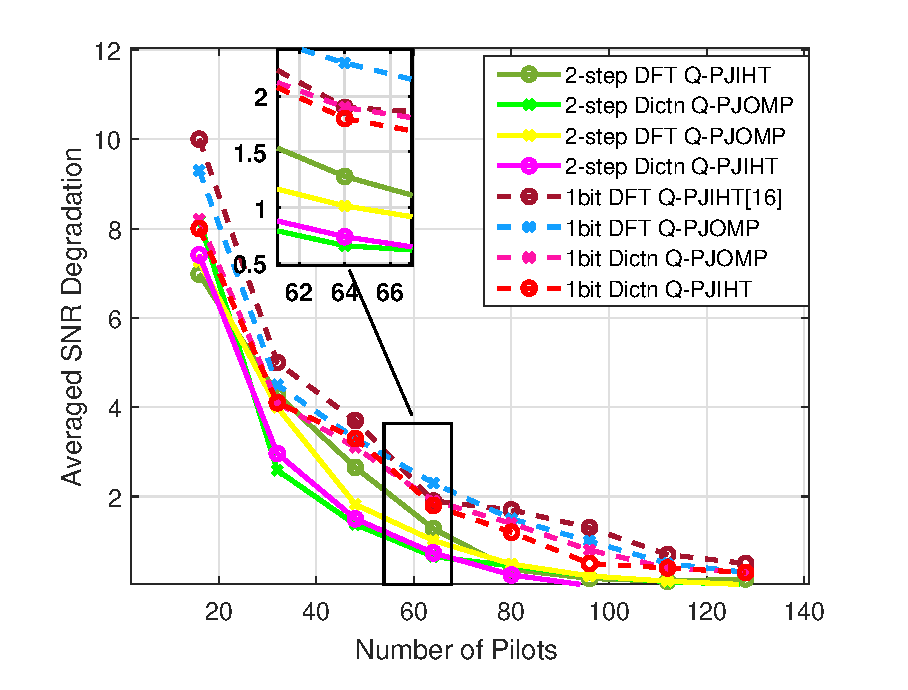
\includegraphics[scale=0.8]{figures/fig_ch_rec/fig2_final.eps}
\caption{Averaged SNR degradation for 1-bit and 2-step quantization using DFT and Dictionary basis  }
\label{Fsnr-deg}
\end{figure}

\begin{figure}[h!]
\centering
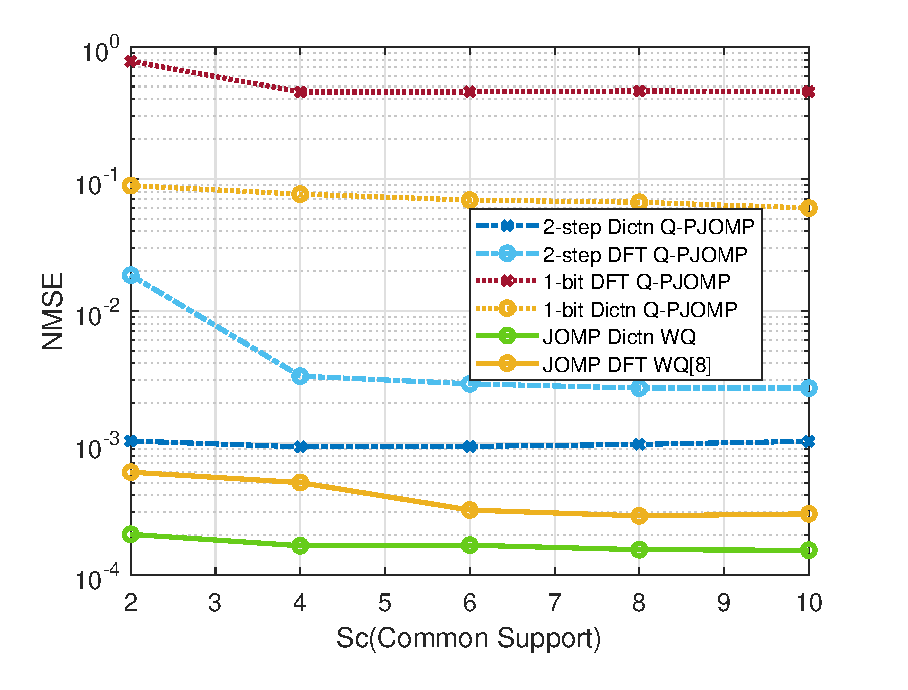
\includegraphics[scale=0.8]{figures/fig_ch_rec/common_support.eps}
\caption{NMSE of CSIT vs common support for 1-bit, 2-step quantization using Q-PJOMP and without quantization(WQ), under P = 45,
$N_t$ = 160, $N_r$ = 2, K = 40, $s_i$ = 17 and transmit SNR = 28 dB.}
\label{sc-jomp}
\end{figure}

\begin{figure}[h!]
    \centering
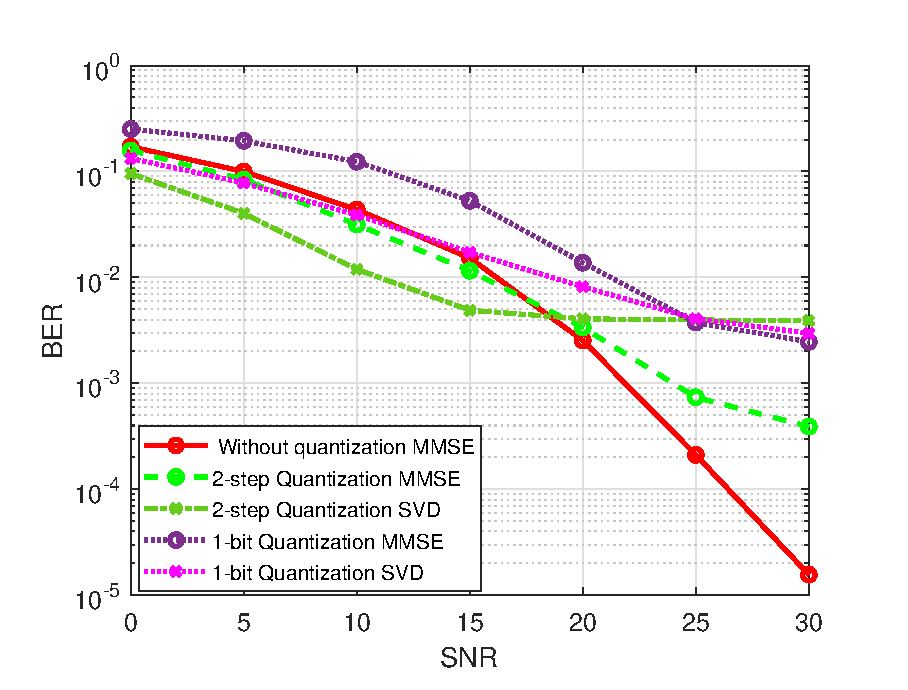
\includegraphics[scale=0.8]{figures/fig_ch_rec/detection-JOMP.eps}
\caption{Averaged Multi-user detection with quantized CSIT based MMSE beamforming (1-bit, 2-step Q-PJOMP) and without quantization (WQ)\label{Fdetection-jomp} } 
\end{figure}
\begin{table} \footnotesize
    \renewcommand{\arraystretch}{1.1}
    \caption{Simulation parameters}
    \label{tabSim}
    \centering
    \begin{tabular}{llr}
        \textbf{Parameter}&\textbf{Symbol}&\textbf{Value}\\
        \hline
        \\
        Transmit antennas & $N_t$&$128$\\
        Receive antennas & $N_r$&$2$\\
        Users            & $K$&$10$\\
        OFDM subcarriers & $N_o$&$256$\\
        OFDM guard interval & $G$&$16$\\
        QAM Modulations & $QAM$&$4$\\
        Multipath channel length & $L$&$6$ \\
        Dictionary length & $M$ & $300$
    \end{tabular}
\end{table}\end{center}

\begin{figure}[h!]
    \centering
    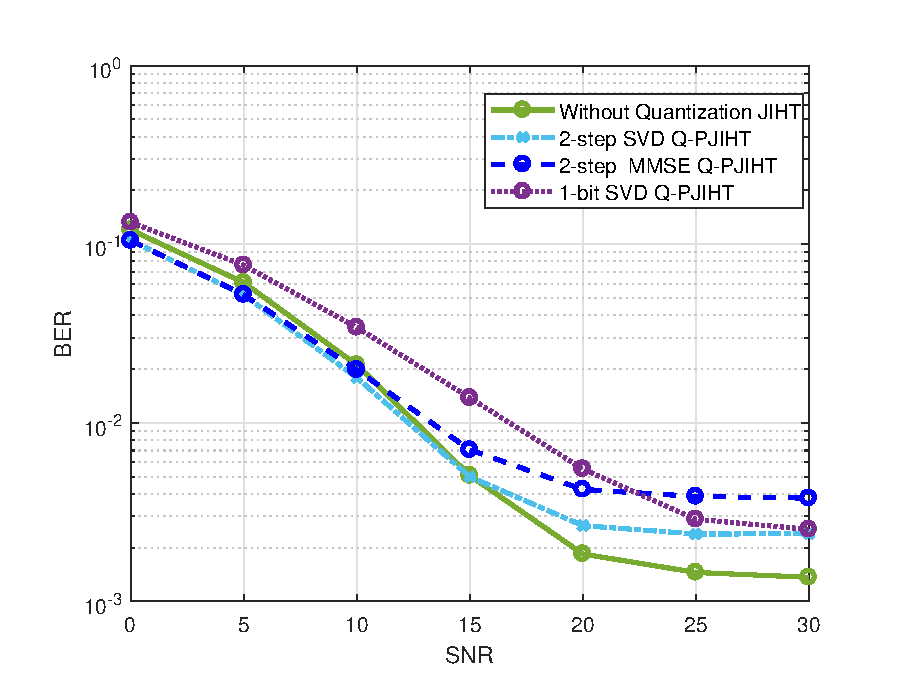
\includegraphics[scale=0.8]{figures/fig_ch_rec/detection_iht.eps}
\caption{Averaged Multi-user data detection with quantized CSIT based beamforming (1-bit, 2-step Q-PJIHT) and without quantization}
\label{Fdetection-JIHT}
\end{figure}

\begin{figure}[h!]
    \centering
\includegraphics[scale=0.8]{figures/fig_ch_rec/JOMP_L.eps}
\caption{Averaged Multi-user detection with quantized CSIT based beamforming (1-bit, 2-step Q-PJOMP) with varying channel taps $L$ }
\label{Q-PJOMP_L}
\end{figure}
We assume a multipath fading channel with a multipath channel length $L_{taps}$ equal to $6$, whose consequent ISI is directly solved by the OFDM guard interval $G$, moreover, the length of $G$ is set to $16$. The joint sparsity $s_c$ and the individual sparsity $s_i$  parameters are chosen to be  $6$ and  $10$ respectively, where $s_c$ and $s_i$ are defined in Sec. \ref{lbDis_JCS}. 
The summary of the discussion is presented in table \ref{tabSim}, which summarizes the system parameters. In the following subsections, the performance analysis is presented evaluating different metrics, i. e., signal to noise ratio (SNR) degradation, normalized mean squared error (NMSE) as in \cite{mainref-joint}  
for the channel state information at the transmitter (CSIT), and bit error rate (BER) while detecting the data at each user terminal. \\
\subsection{SNR Degradation}
In this subsection, we present the averaged SNR loss obtained using the estimated channel with different numbers of pilot symbols as in \cite{mainref-1bit}. For channel $\mathbf{H}_i$ and its estimate $\mathbf{\hat{H}}_i$, the precoder $\mathbf{w}_i$ is the maximizer of $\|\mathbf{w}_i^H \mathbf{H}_i \mathbf{H}_i^H \mathbf{w}_i\|_2^2$ and $\mathbf{\hat{w}}_i$ is the maximizer of  $\|\mathbf{\hat{w}}_i^H \mathbf{\hat{H}}_i \mathbf{\hat{H}}_i^H \mathbf{\hat{w}}_i\|_2^2$, respectively. The overall SNR loss in $dB$ can be calculated as follows\textcolor{black}{:}
\begin{equation}
    \text{SNR}_{deg}=10\text{log}_{10}\frac{\|\mathbf{w}_i^H \mathbf{H}_i \mathbf{H}_i^H \mathbf{w}_i\|_2^2}{\|\mathbf{\hat{w}}_i^H \mathbf{\hat{H}}_i \mathbf{\hat{H}}_i^H \mathbf{\hat{w}}_i\|_2^2}
    \label{snr_deg}
\end{equation}
Around 200 simulations have been performed to obtain the channel estimate $\mathbf{\hat{H}}_i$ and the precoder $\mathbf{\hat{w}}_i$, which are used in equation (\ref{snr_deg}) to calculate the averaged SNR degradation. Fig. \ref{Fsnr-deg} analyzes the SNR degradation employing Q-PJIHT or Q-PJOMP having 1-bit or  2-step quantization using either DFT or dictionary-based sparsifying matrices. It can be observed that when the feedback overhead approaches $48$ pilots, the SNR degradation exceeds $2$ $dB$ in 1-bit method \cite{mainref-1bit}, which is more than the degradation achieved by the proposed 2 bit Q-PJOMP. Overall, the proposed 2-step Q-PJOMP outperforms the other schemes. 
There are numerous reasons for the better performance of the proposed algorithm: firstly, we have selected a better CS algorithm, i.e., Q-PJOMP, that is more efficient than the IHT based algorithm (Q-PJIHT).   Secondly, since the choice of $\eta$ is critical in IHT \cite{Aiht}, a flexible gradient step size $\eta$ is employed in the Q-PJIHT algorithm. The $\eta$ is used as per sparsity level requirements in each iteration, contrary to a fixed-size of $0.01$  used in \cite{mainref-1bit}.  Thirdly, the 2-step quantization preserves both amplitude and phase information rather than having only direction information as in \cite{mainref-1bit}. Finally, our system employs a dictionary-based sparsifying matrix, which is more robust to estimate the channel as compared to earlier research works \cite{mainref-1bit,mainref-joint}.  This results in better performance with the reduced number of measurements and a fewer number of bits\cite{ourwork}.
Fig. \ref{Fsnr-deg} compares the proposed Q-PJOMP/Q-PJIHT solutions with a 1-bit feedback method  \cite{mainref-1bit}. It can be easily noticed that with $64$ pilots in the magnified view, the proposed quantized feedback  Q-PJOMP with a dictionary-based approach surpasses the performance of almost all feedback based algorithms. Moreover, by increasing the number of pilots, the SNR loss drops down to almost zero for all the solutions. Finally, focusing on the proposed Q-PJOMP method in Fig. \ref{Fsnr-deg}, the 2-step quantization reflects less degradation as compared to the 1-bit quantization.
\subsection{CSIT NMSE analysis Versus common support}
 Fig. \ref{sc-jomp} illustrates the normalized mean square error (NMSE) of CSIT while increasing the common support $s_c$, under the same simulation parameters as in \cite{mainref-joint} for the comparison purpose. The simulation parameters are enlisted as followed: transmit pilot P = 45,
$N_t$ = 160, $N_r$ = 2, K = 40, $s_i = 17$ and transmit $SNR = 28$ dB.
NMSE has been calculated as follows:
\begin{equation}
    \text{NMSE} =\text{E}  \left(\frac{\|\mathbf{H}_i-\mathbf{\hat{H}}_i\|_F}{\|\mathbf{H}_i\|_F} \right)
\end{equation}
The individual and joint sparsity levels are generated using the spatial channel model (SCM)\footnote{3rd generation partnership project(3GPP) and the international telecommunication union(ITU) has developed a spatial channel model(SCM) to model various urban and rural propagation scenarios \cite{SCM}} as in \cite{mainref-1bit,mainref-joint}. Fig. \ref{sc-jomp} reveals as the common support $s_c$ increases among users, the system performance improves, i. e., when the channel between users is more correlated.  These results reinforce our argument that 2-step quantization provides a better estimation than a 1-bit scheme.  It can be observed that the proposed JOMP with a dictionary basis without quantization (WQ) gives better performance than DFT based J-OMP \cite{mainref-joint}.
\subsection{ BER Analysis}
Fig. \ref{Fdetection-jomp} and \ref{Fdetection-JIHT} present the comparison of BER  versus SNR for data detection techniques utilizing SVD and MMSE based beamforming. The channel estimate required for beamforming is obtained using quantized feedback and applying CS techniques such as J-OMP and J-IHT. Moreover, the beamforming obtained without using quantized feedback is presented for comparison purposes.  It is worth noting in Fig. \ref{Fdetection-jomp} that beamforming based on channel estimate obtained using 1-bit feedback and Q-PJOMP has a wider gap as compared to the algorithms without quantization. Moreover, Q-PJOMP with MMSE based precoding gives better results than its SVD counterpart.  \ \
On the contrary, Fig. \ref{Fdetection-JIHT} illustrates that the proposed Q-PJIHT with MMSE precoding performs more inferior as compared to Q-PJIHT with SVD.   By comparing Fig. \ref{Fdetection-jomp} and \ref{Fdetection-JIHT}, it can be observed that Q-PJOMP exhibits better performance as compared to Q-PJIHT, for all the cases with and without quantization. Fig. \ref{Q-PJOMP_L} shows the effect of multipath fading over data detection by employing MMSE beamforming utilizing quantized 1-bit and 2-step feedback using Q-PJOMP based channel estimates.  It can be observed, that as expected by increasing the number of channel taps from $2$ to $5$ the BER performance in all cases is reduces, though the proposed technique yields the improved results.
\subsection{ Computational Complexity Analysis}
Table \ref{tab:comp_time} presents the comparison of computational time per user for 2-step and 1-bit Q-PJOMP/Q-PJIHT. Three different transmit antennas setting has been considered: $N_t=[50, 100, 150]$. 
As expected, the computational time increases with the number of transmit antennas. Furthermore, the 2-step algorithms (Q-PJOMP/Q-PJIHT) are more expensive than 1-bit methods. This is due to the processing of the channel amplitude information, and rebuilding complex pilots from both amplitude and direction information, nevertheless, the analysis reveals that the difference is not very significant. 
Finally, comparing Q-PJOMP with Q-PJIHT, iterative hard thresholding based algorithms are generally much slower than the orthogonal matching pursuit based techniques, since they require a certain number of iteration to reach an optimal point.   
\begin{table}[h!]
    \caption{ COMPUTATION COMPLEXITY COMPARISON FOR MU-MASSIVE MIMO UNDER PARAMETRIC SETTING  P = 45, N = 2, K = 40, $s_c$ = 9, $s_i$ = 17, P = 28 dB AND $N_t$= 50,100, 180. }
\label{tab:comp_time}
\centering
%\addtolength{\tabcolsep}{-2pt}
 \begin{tabular}{||c |c |c |c ||} 
 \hline
Time(s)&$N_t$=50&$N_t$=100&$N_t$=150\\ [0.9ex] 
 \hline\hline
 2-step Q-PJOMP&$1.2 \times10^{-3}$&$1.4 \times10^{-3}$ & $1.6 \times10^{-3}$ \\ [0.9ex]
 \hline
 1-bit Q-PJOMP& $9.24\times10{-4}$&$1.2 \times10^{-3}$& $1.3\times10^{-3}$ \\[0.9ex]
 \hline
 2-step Q-PJIHT& $6.86\times10^{-2 }$& $7.19\times10^{-2 }$&$7.38\times10^{-2 }$  \\[0.9ex]
 \hline
 1-bit Q-PJIHT&$5.82\times10^{-2 }$& $6.94\times10^{-2 }$&$7.02\times10^{-2 }$ \\[1ex] 
 \hline
\end{tabular}
\end{table}

\section{Conclusion}
We have presented distributed compressed sensing based channel estimation techniques for the partially joint channel in a massive MIMO system.  Especially, a novel Q-PJOMP and Q-PJIHT based channel estimation algorithms utilizing limited quantized feedback are proposed. The proposed system reduces training and feedback overhead by employing a fewer number of pilots along with a limited number of feedback bits for channel estimation. Moreover, the channel is jointly recovered for all users by applying DCS at BS from 2-step quantized feedback. \\
The results revealed that SNR degradation with 2-step quantized feedback is less than 1 dB for 64 pilots. Furthermore, as the number of pilots grows, the SNR degradation approaches closer to zero. Additionally, the presented dictionary-based system aids in reducing the training and feedback overhead. This is achieved by exploiting an improved CS  algorithm and pilot design. Finally, when the channel among users is highly correlated and exhibits added common support, the jointly estimated channel at BS will reduce the computational resources and time. The future work comprises of extending the proposed massive MIMO scheme to localization issues for improving performance  \cite{LocalizationICC2013,LocalizationTVT2016}, this could be achieved by exploiting a large number of serving antennas.

%%%%%%%%%%%%%%%%
 %Chapter 6
%%%%%%%%%%%%%%%%

%\chapter{Beamforming Galvanic Coupling}
\section{Introduction} \label{sec:intro}
Assistive technologies allow humans to augment their natural abilities and restore physiological functions lost due to illness or injury. An example of today's closed loop communication with man-machines interfaces involves controller-driven artificial limb stimulation based on muscle exertion levels. Embedded sensors in the tissue detect the muscle stress and communicate their readings back to the controller for precisely computing the needed stimuli for limb movement ~\cite{cyborgs}. This paradigm of interconnected implants results in an Intra-Body Network (IBN) that allows internal physiological data to be gathered in real time and analyzed off site, thereby transforming personalized medicine.
However, the state of the art for Intra-Body Communication (IBC) relies on high frequency radio (RF) signals. RF incurs significant energy costs owing to high absorption within the human tissues that are composed of $40$-$65\%$ water. Additionally, emitted RF signals may extend to several feet around the body, creating privacy risks. We use an alternative wireless architecture for IBNs using galvanic coupling (GC), in which low or medium frequency ($100\,\mathrm{kHz}$-$1\,\mathrm{MHz}$) and weak ($\leq 1\,\mathrm{mW}$) electrical currents are modulated with data and directly coupled to the tissue. The privacy risks related to RF are eliminated by using GC in IBNs since the signals do not propagate outside the skin layer \cite{teshome}. GC is a method of IBC also commonly referred to as human body communication (HBC). For consistency we will continue to refer to it as an IBC method. We call this paradigm as GC-IBN, and it consumes two orders of magnitude less energy than RF signals \cite{tbiocas}.

  \noindent $\bullet$ \textbf{Problem:} The GC-IBN architecture is composed of multiple embedded implants that transmit their sensed data to an on-skin node, called as a \textit{relay}. The muscle to muscle (M-M) path offers lowest path-loss ($\approx 19\ \mathrm{dB}$) and hence, is ideally suited for communication across different implants in the same muscle layer~\cite{tbiocas}. However, implant to the surface relay communication needs to traverse several different tissue boundaries that have higher path loss, for e.g, the muscle to skin (M-S) path has $\approx 38\ \mathrm{dB}$ of loss. How to send these signals to the relay with the least overhead (even if the baseline  GC performance is much more energy efficient than RF) with high SNR remains an open challenge~\cite{aniso,ICNIRP}. Further, existing standards like IEEE 802.15.6 designed for implant communication use contention-based medium access with the possibilities of collisions, back-off and packet loss. Such events incur energy costs of re-transmissions and idle-listening, which we wish to avoid in IBNs.

\begin{figure*}[h]
 \centering
\includegraphics[width=\textwidth]{figures/GC_beamforming/expr2.pdf}  
%[width=18cm,height=6.1cm]{figs/expr2.pdf}  
 \vspace{-2mm} 
 \caption{\label{fig:expr} (left) Human fore-arm GC-IBN with muscle implants and surface relay; (right) Phantom-based testbed using Arduino}
 \vspace{-5mm}
  \end{figure*}

\noindent $\bullet$ \textbf{Proposed Approach:} We propose a light-weight cross-layer framework that combines compressive sensing code division multiple access (CS-CDMA) with distributed beamforming in narrow band channels, while ensuring that computational costs are delegated to the relay. We define beamforming in the context of this near-field application as the phase tuning of GC signals to achieve constructive interference between multiple implant transmissions and improve the SNR at the relay. The implants themselves simply record and forward data, with the relay being responsible for both the CDMA decoding (to extract the actual sensed value) and tuning of the beam-steering matrix (for directional communication with high SNR). Existing far-field beamforming techniques cannot be applied for GC-IBN, as the receiver is placed in the near-field of the low frequency transmitter, separated only by a few centimeters. 

\begin{table}[b]
\vspace{-6mm}
\centering
\caption{\label{tab:overview} Variable definitions and ranges}
\vspace{-3mm}
\footnotesize
\begin{tabular}{l|l}
\toprule
Variables & Definitions\\
\midrule
$M$, $R$ \& $m_i$ & Total number of nodes, Relay \&  Implant $i$ \\
M-M, M-S, S-M & Paths: Muscle-muscle, muscle-skin, Skin-muscle\\
$\overrightarrow{H}$, $\overrightarrow{E}$ & Instantaneous magnetic  and electric fields\\
$\theta_i$, $\phi_i$ & Azimuth and  elevation angles\\
$r_i$ & Distance between 2 points in spherical coordinates\\
$AF$ & Array factor\\
$g^p$ & Gain in path p;  $ge$ - $\overrightarrow{E}$ gain; $gh$ -  $\overrightarrow{H}$ gain \\
$\psi$, $\gamma$  & Phase shift and Frequency offset \\
$f,w,\triangle f$ & Frequency, angular frequency and bandwidth\\
$c \& c'$ & Speed of EM signals in vacuum and tissue \\
$w^s, w^p, w^t$ & Weights for safety, phase match \& steering \\
$c_{ik}$ \& $b_{i,n}$ & $k^{th}$ bit of Walsh code for $m_i$ 
\& $n^{th}$ bit of $m_i$\\
$\eta_m$ & Required data rate for $m_i$, $\forall i\in\{1,..,M\}$\\
$P_i$ & Transmit power consumed in $m_i$, $\forall i\in\{1,..,M\}$ \\
$Pr^R$ \& $P^S$ & Received  power in R \& Safe transmit power\\
$\delta^{M\text{-}S},\delta^{M\text{-}M}$ \& $\sigma$ & SNR in path M-S and M-M \& Noise variance\\
$N_o$ & Gaussian distributed noise P.S.D $\in (0,\sigma^2)$ \\
\bottomrule
\end{tabular}
\end{table}


\begin{table}[h]
\centering
\vspace{2mm}
\caption{\label{tab:result1} Power consumption for 1 bit with $E[P]=0.5mW$}
\vspace{-2mm}
\small
%\scalebox{0.7}{
\begin{tabular}{ccccc} 
\toprule
M	& $Pr$ & $Pr(W^p)$	& $aPt$ &	Life\\
	& $(\mu W)$ & $(\mu W)$	& (mW) & (weeks)\\
\midrule
1	& 	0.9	& 	0.92 & 	0.5 	&	10\\
2	&	1.9	&	1.93&	0.23	&	21\\
4	&	3.67	&3.71	&0.12&		40\\
6	&	5.37&	5.49&	.085	&	59.5\\
10	&	8.94&	9.11&	0.05	&	98.8\\
%12	&	10.5&	10.8&	0.04    &	116.9\\
14	&	12.4&	12.7&	0.03	&	137.9\\
\bottomrule
\end{tabular}
\end{table}	 

The end to end procedure is described as follows: The relay assigns unique CDMA codes to the implants. The latter store the sensed values and create modulated codewords using these assigned quasi-orthogonal codes. Using the high-gain M-M channel, the implants inform a designed aggregator, placed in the same muscle tissue, of their individual codewords. Such aggregator records the received CDMA-coded data structure created by the simultaneous transmissions of multiple sensors on the same channel. Note that there is no decoding step at this point to save energy and the aggregator simply broadcasts back this cumulatively received codeword to the implants. By using distributed beamforming, each implant then transmits this codeword to the relay. Through this process, the energy consumed per implant is reduced, greater directional transmission is obtained and the relay receives much higher SNR than what would have been possible via a single transmission. The final CDMA decoding is then performed at the relay, and the individual sensor data is then extracted. The entire 2-step process of (i) exchanging individual codewords among peer implants, and (ii) beamforming to the relay, is collision-free.
  
\noindent $\bullet$ \textbf{Contributions:} The main contributions of this work are:

\noindent 1. We propose a CS-CDMA-based cross-layer approach that allows implants in the muscle to communicate with surface relays using galvanic coupling, which is  collision-free and has reduced complexity of decoding.

\noindent 2. We present the first formulation of near-field distributed beamforming in the body that accounts for specific tissue paths, constraints of tissue safety ($\le 25\, mA/m^2$)~\cite{ICNIRP} and increases SNR at the surface relays. We present tissue-phantom and Arduino-based proof of concept of how constructive phase addition is possible within the body.

\noindent 3. We use empirically obtained data sets to model the body channel and evaluate the effectiveness of our approach using an extensive finite element based simulation using MATLAB-generated mathematical models. 

\noindent 4. We demonstrate GC-beamforming through the muscle, fat and skin layers on a testbed using National Instruments Universal Software Radio Peripherals (USRPs) where we transmit data from multiple sensors through a human tissue phantom. Our measurements of received signal strength and BER at the demonstrate the merits of using beamforming within a physical intra-body sensors communication system.

\section{Background and Related Work}\label{sec:bg}
Existing standards for Wireless Body Area Communication (WBAN), including IEEE 802.15.4 based LR-WPAN (Zigbee), IEEE 802.15.6 Human Body Communication (HBC) standard and  Bluetooth low energy (BLE), assume that implants are similar to classical over-the-air wireless sensor networks. 

This is because in both cases, the nodes are battery powered, have small form factors, with low on-board resources. Classical CSMA/CA \cite{ieee802,backoff} and channel hopping used in these standards impacts definite time of delivery, energy efficiency, and is unable to handle sudden spikes in traffic. The frame-length and inter-frame spacing are designed for high frequency signal propagation in the air medium over long distances (\textgreater\textgreater  $2\,\mathrm{m}$), rather than the low frequency short range communication (\textless \  $50\,\mathrm{cm}$) inside the body. Other overheads such as handshakes, channel sensing, scheduling, transitions from frequent sleep and wake-up states, among others, increase the processing complexity. An alternative form of intra-body links established using ultrasonic signals suffer from high multi-path delay and complex circuitry.

We note that the low rate and sparse traffic generated by implants under normal physiological conditions may become bursty when an abnormal event is observed,  limiting utility of both contention-based and reservation-based access techniques. Hence, for contention and reservation-free access, we advocate the use of \cite{cdma} that enables concurrent transmissions. However, CDMA multiplies the energy costs by using a high rate code, which in turn contributes to the net energy consumed per unit of useful data. Thus, due to the sparse nature of sensed data, we apply a combined CS-CDMA procedure to reduce the transmission time and energy. CS based solutions have been already successfully applied \cite{candes} -\cite{alesii} to both recover data and identify the transmitters. In this paper, we further combine energy efficient CS-CDMA solution with smart energy-focusing strategies. Seminal contributions for conventional beamforming in far-field, high frequency signals exist~\cite{UWBBF}. However, the problem of beamforming for near-field and narrow band signals in a heterogeneous tissue-like medium has not been demonstrated so far, particularly for the low frequency signals (\textless $1\ \mathrm{MHz}$) used in GC-IBN. Coordinated beamforming using multiple separate antenna elements may be possible in many applications where implants are placed in close proximity of each other, such as neuro-muscular stimulators or orthopedic sensors that merits further investigation on this topic~\cite{cyborgs,ortho2}.
\begin{table}[h]
\caption{Conductivity and relative permittivity of three layers of phantom tissue \cite{dielec}}
\begin{center}
\begin{tabular}{ c||c|c|}
&Conductivity[S/M] & Relative Permittivity\\
\hline
Skin & 0.0030479 & 1076.3 \\
\hline
Fat & 0.024769 & 38.134 \\
\hline
Muscle & 0.42782 & 4339.3 \\
\hline 
\label{dielectric}
\end{tabular}
\end{center}
\vspace{-2pt}
\end{table}
\section{Tissue Phantom Experiments}
\label{sec:exp}
As a motivation for choosing beamforming, we use a tissue phantom-based preliminary testbed (see  Fig.~\ref{fig:expr}(a) for the block diagram describing the setup and Fig.~\ref{fig:expr}(c) for a snapshot) to analyze the constructive and destructive combination of concurrently propagating signals through tissue. We use a dielectrically equivalent human tissue phantom with a skin, fat and muscle layer purchased from SynDaver\textsuperscript{\textregistered}. The $20$ x $20$ x $3.1$  $cm^3$ phantom was constructed from salt, water and fiber and was ordered specifically for GC tests to have the dielectric values presented in Table \ref{dielectric}. The three layers (skin, fat, muscle) were stitched together by the manufacturer.

We use pulse width modulated (PWM) signals at $100\, \mathrm{kHz}$ and $0.5\,\mathrm{V}$ generated by a pair of Arduino Uno boards, whose phase is controlled by a common synchronization pulse generated by MATLAB. The PWM signals are passed through a safety circuit (Fig.~\ref{fig:expr}(b)) in order to limit the signal within the safe bound (=$1 \ mA$) we set based on the suggestion by ICNIRP~\cite{ICNIRP} %KRC mention this bound
and then coupled to the muscle phantom (mimicking implants) by two pairs of electrodes. The transmitters are separated by $16\,\mathrm{cm}$ and the electrode pair in each transmitter is separated by $4\,\mathrm{cm}$. A pair of receiving electrodes is positioned on the surface skin of the phantom at $15\,\mathrm{cm}$ from each transmitter, and connected to an oscilloscope to observe the output voltage. For each signal, the corresponding Thevenin-equivalent circuit is built to measure the output power level. 

When only one Arduino is transmitting a power of $0.25\,\mathrm{mW}$, the maximum average output power ($Pr_{max}$) we observed is $3\,\mathrm{\mu W}$. When two transmitters are transmitting concurrently, and in perfect phase alignment (Fig~\ref{fig:expr}(d)), $Pr_{max}$ is $6\,\mathrm{\mu W}$, which is double than the case of a single transmitter. This shows that the constructive signal addition is beneficial. However, when the input signals are out of phase (Fig~\ref{fig:expr}(e)), $Pr_{max}$ $\approx 2.6\,\mathrm{\mu W}$, which is lower than the case of a single active transmitter, showing the impact of destructive signal combination. When the signals are partially out of phase (Fig.~\ref{fig:expr}(f)), $Pr_{max}$ becomes $ \approx 4.3\,\mathrm{\mu W}$. The set-up includes the mutual coupling effect from multiple transmitters and thus mimics the real scenario. Our experiments motivate the potential benefits of phase-alignment based beamforming within heterogeneous tissues using GC-coupled links. We extend this testbed further in Section \ref{sec:implement} where the constructive and destructive combination of galvanic signals is explored further by applying the weights calculated in the following section.  %Using these results, we proceed with the design of beamformed CDMA based MAC design for galvanic coupled implants communication.

\section{Beamforming for Implant Communication} \label{sec:bf}

In this section we develop the theoretical background for beamforming using an array of implants acting as distributed antennas. We assume that each implant has a common CDMA modulated codeword $\tilde{\mathbf{d}}$ that is created and disseminated by the aggregator back to the implants and focus on the formulation of the beamforming weights. In preparation to that, we first explain the channel between implants and from the implant to the relay in Sec.\ref{channel}. Following that, Sec.\ref{nf} justifies the use of near-field transmissions followed by a description of the electric field of one the GC transmitter in Sec. \ref{electrode_pattern}. We extend the electric field analysis to the array-structure resulting from multiple nearby implants, and then calculate the cumulative received power at the surface relay in Sec.\ref{no_beam_array}. Then, we derive the complex weights to limit the beam-formed signal within the safe power limit, focus the signal strength at the receiver and devise a method to steer the input signals from each node in the desired direction in Sec.\ref{bf}.

\subsection{Implant network and 3-D tissue channels} \label{channel}
We assume a set of $M$ uniformly distributed co-planar implants $\{m_1,..,m_M\}$ arranged in muscle tissue linearly, at locations $(r_m,\theta_m,\phi_m)$, where $r_m\in[0,r_{max}]$ is the maximum distance of separation in muscle. Let $\theta_m\in [0,2\pi]$ be the azimuth angle measured from the X-axis, and $\phi_m\in[0,\pi]$) be the elevation angle measured from the Z-axis, respectively, all in radians, with the origin at $(0,0,0)$ as shown in Fig.\ref{fig:angles}. The number of implants in a given body part can vary from $1$ to $M$, for e.g., neural stimulation uses more than $50$ implanted cuffs in one limb \cite{cyborgs,arrayelectrodes}. The external relay node $R$ on the body surface controls the actions of the implant-group by issuing synchronization pulses, aggregating their information, providing receiver feedback for beamforming and decoding the sensed values \cite{infocom}. It is located at ($r_R,\theta_R,\phi_R)=(T, 0,0)$, where $T$ is the tissue thickness separating $R$ and the ($r,\theta$) plane at $\phi$=$\pi/2$, in which the implants are embedded. We assume identical path loss for all the implants and the tissue channel has negligible signal reflection, scattering, or shadowing~\cite{tbiocas}.

\noindent$\bullet$ \textbf{Implant-Implant channel:} The channel between a given muscle implant ($m_i$) and another peer implant ($m_j$) that  communicates along the M-M path is specified by the gain $gx_{ij}^{M-M}$, and phase shift $\psi x_{ij}^{M-M}$ for a field $x\in[\overrightarrow{E},\overrightarrow{H}]$. Here,  $\overrightarrow{E}$ is the electric field and $\overrightarrow{H}$ is the magnetic field. The channel gain and phase are obtained as
$gx_{ij}^{M\text{-}M}\text{=} f_1^{M-M}(||r_{ij}||,\theta_{ij}) \, \&\ $
$\psi x_{ij}^{M-M}\text{=} f_2^{M\text{-}M}(||r_{ij}||,\theta_{ij})$
where, $\theta_{ij}$ is the relative azimuth angle between $m_i$ and $m_j$, and $||r_{ij}||$ is the separation between implants ($m_i$) and ($m_j$) through the M-M path estimated as $||r_{ij}||\text{=}\sqrt{r_i^2+r_j^2-2r_ir cos(\theta_i-\theta_j)}$. The relative elevation angle $\phi_{ij}$=$0$ as the implants are assumed to be co-planar. Note the above formulation can be trivially extended for non co-planar muscle implants, though we leave out this case for space limitations.\\
\noindent$\bullet$ \textbf{Implant-Relay channel:} The channel between the implant ($m_i$) to relay $R$ communication through the M-S path is given in terms of gain ($gx_{iR}^{M-S}$) and phase shift introduced by the tissue path through muscle-fat-skin interfaces ($\psi x_{iR}^{M-S}$) for a field $x$, written as,
\begin{equation}\label{e:g}
gx_{iR}^{M\text{-}S}\text{=} f_1^{M\text{-}S}(||r_{iR}||,\theta_{iR},\phi_{iR})\ \&
\end{equation}
\begin{equation} \label{e:psi}
\psi x_{iR}^{M-S}\text{=} f_2^{M\text{-}S}(||r_{iR}||,\theta_{iR},\phi_{iR})
\end{equation}

where $\theta_{iR}$ and $\phi_{iR}$ are angles defined similarly between $m_i$ and $R$. $||r_{iR}||$ is the separation between implant ($m_i$) and relay through the M-S path estimated as $||r_{iR}||=\sqrt{r_i^2+r_R^2-2r_ir_R[A+B]}$, 
where $A$=$sin(\theta_i)sin(\theta_R)cos(\phi_i$-$\phi_R)$ and $B$=$cos(\theta_i)cos(\theta_R)$, and $P \in \{M-M,M-S,S-M\}$ is the path of the signal. The functions $f_1^{M\text{-}M}$, $f_2^{M\text{-}M}$, $f_1^{M\text{-}S}$ and $f_2^{M\text{-}S}$ are obtained using the channel models for $\overrightarrow{E}$ and $\overrightarrow{H}$ fields in \cite{tbiocas}.
\begin{figure}[t]
 \centering
 %\vspace{-1mm}
\includegraphics[width=8cm,height=5cm]{figures/GC_beamforming/angles.png}  
 \vspace{-3mm}
 \caption{\label{fig:angles} Spherical coordinate system with an implant and a relay}
  \vspace{-7mm}
  \end{figure}
  

\subsection{Near-field signal propagation}\label{nf} Signals impinging on a receive antenna are typically assumed to have planar wavefront. This assumption is not valid in GC-IBN for the following reasons: First,  GC-IBN uses the operating frequency of $100\,\mathrm{kHz}$ to $1\,\mathrm{MHz}$, with a wavelength ($\lambda$) of $2E3$ to $3E3\,\mathrm{m}$. Second, the size of the electrodes used in implants range from  few $\mu\mathrm{m}$ to $\mathrm{mm}$. 
The far-field range of such small electrodes is given by $r\geq \frac{\lambda}{2\pi}$, i.e.,  $r\geq 3.1E2$ for $100\,\mathrm{kHz}$ and $4.7E2\,\mathrm{m}$ for $1\,\mathrm{MHz}$. However, the possible separation between the transmitter and receiver in GC-IBN can be at most $30\,\mathrm{cm}$ based on measurements in~\cite{tbiocas}. Beyond this range, the received SNR is too low for messages to be reliably decoded. Thus, GC-IBN communication is confined to the near-field range.

Having classified the GC-IBN communication as near-field, we proceed to explain the assumption of a spherical expansion of the electric field. The radiation pattern concept, usually referring to far-field communications, is borrowed to explain the near-field pattern of our electrodes in this case. Consider the electric field ($\overrightarrow{E}_i$) that is proportional to the voltage ($V_{in}$) applied to the input electrodes that couple the GC signal to muscle. The magnetic field ($\overrightarrow{H}_i$) is proportional to the applied current ($I_{in}$) in the same implant $m_i$. The instantaneous $\overrightarrow{E}_i$ and $\overrightarrow{H}_i$ field strengths in the far field decrease inversely with distance (inverse-square law) and carry a relatively uniform wave-pattern, where the received signal is assumed to have constant frequency and infinite plane of constant phase and constant peak-to-peak amplitude normal to the phase velocity vector. These fields are also orthogonal to each other.
As opposed to this, in the near-field,  $\overrightarrow{E}_i$ and $\overrightarrow{H}_i$ field strengths falls exponentially with increasing distance from the source, contrary to the inverse-square law. 
Moreover, they can exist independent of each other with their field distributions depending on the tissue structure complexity without a strictly defined decreasing relationship. The electric and magnetic field components are assumed to expand spherically through the tissue.

\subsection{Electric field pattern based on tissue orientation} \label{electrode_pattern}

The current coupled to the input electrodes of an implant is assumed to introduce a nearly isotropic radiation pattern in the surrounding tissue. However, higher conductivity along the longitudinal axis of the muscle tissue results from the continuous muscle strands that are oriented similarly. Coupled with the layered structure of such tissues in the transverse direction, the electrical field is $\approx \sqrt{2} $ times stronger in the longitudinal direction of the muscle tissue \cite{aniso}. To incorporate this tissue anisotrophy, we model the spherical wave-front of electric field ($\overrightarrow{E}_i$) and magnetic field ($\overrightarrow{H}_i$) as follows.
\begin{equation} \label{eqn:E}
\overrightarrow{E}_i \text{=}V_{in}\times\begin{cases}  
sin\left(\frac{\pi}{2} - \frac{\phi}{4} \right),  & \forall\,\phi \in [0,\frac{\pi}{2}]\\
sin\left(\frac{\frac{\phi}{4} - \pi}{2} \right),  & \forall\,\phi \in [\frac{\pi}{2},{\pi}]
\end{cases}
\end{equation}
\begin{equation} \label{eqn:H}
\overrightarrow{H}_i \text{=}I_{in}\times\begin{cases}  
1.7-sin\left(\frac{\theta}{2} + \frac{\pi}{4} \right),  & \forall\,\theta \in [0,\pi]\\
1.7-sin\left(\frac{\theta-\pi}{2} + \frac{\pi}{4} \right),  & \forall\,\theta \in [\pi,2\pi]
\end{cases}
\end{equation}

For the instantaneous $\overrightarrow{E}_i$ and $\overrightarrow{H}_i$ fields emanating from $m_i$,  the instantaneous energy flux density caused in the surrounding tissue is expressed as Poynting vector: $\overrightarrow{P}_i^T = \overrightarrow{E}_i \times \overrightarrow{H}_i$, where, the real part denotes the power flow and imaginary part represents the reactive near-field of antenna \cite{mikki}. Equations \ref{eqn:E} and \ref{eqn:H} are derived based on the angles where the electric and magnetic field intensity is maximized. They are maximized in the longitudinal direction of the muscles. Equation \ref{eqn:E}, for example, shows the maximization of the energy in the direction of $\phi=90^o$ from the electric field direction, which corresponds to the direction of the muscle layer (Fig. \ref{fig:multi}(b). Similarly, the energy is maximized in $\theta=0^o$ and
$\theta=180^o$ directions for the magnetic field which also correspond to the longitudinal axis of the muscle layer (parallel to the skin) (Fig. ~\ref{fig:multi}(c)).
The field pattern for the implant $m_i$ during transmission is shown in Fig.~\ref{fig:multi}(a).  

\subsection{Received signal at the relay without beamforming} \label{no_beam_array}
The received near-field signal at $R$ due to transmissions by source $m_i$ can be determined  by modeling the propagation behavior through tissue channel independently for $\overrightarrow{E}$ and $\overrightarrow{H}$ fields as 
\begin{equation}
\overrightarrow{Pr}_i^R = \overrightarrow{E_i^R} \times \overrightarrow{H_i^R}
\end{equation}
where  
$\overrightarrow{E_i^R}$ = $\overrightarrow{E_i}.$ 
$ ge_{iR}^{M\text{-}S} e^{j\omega \left(\psi e_{iR}^{M\text{-}S}+\gamma e_{iR}^{M\text{-}S}\right)}$, $\omega/2\pi$ is the operating frequency and can be written as, \noindent $\displaystyle \overrightarrow{H_i^R}$=$\overrightarrow{H_i} .gh_{iR}^{M\text{-}S} e^{j\omega \left(\psi h_{iR}^{M\text{-}S}+\gamma h_{iR}^{M\text{-}S}\right)}$ and $\gamma_{iR}^{M\text{-}S}$ is the effect of drift in frequency and phase offset. 
We consider $M$ co-planar implants transmitting simultaneously whose positions are uniformly distributed around the reference point with distribution $\displaystyle \frac{r_{max}}{\sqrt{2}}$. The $ge$ and $gh$ values for different tissue path are obtained from the HFSS based finite element simulation model in \cite{tbiocas}.
We define the term \textit{array factor} as the net received signal pattern at the receiver resulting from multiple concurrent transmissions from the array of implants.
For the $\overrightarrow{E}$ and $\overrightarrow{H}$ fields in the uniformly distributed planar implant array, the respective array factors can be written as,
\begin{equation}
E[AF_E] =\frac{1}{M  } \sum_{i=0}^{M-1} \overrightarrow{E_i}ge_{iR}^{M\text{-}S} e^{j\omega \left(\psi_{iR}^{M\text{-}S}+\gamma_{iR}^{M\text{-}S}\right)} \  \&  
\end{equation} 
\begin{equation} \label{e:Harray}
E[AF_H] =\frac{1}{M  } \sum_{i=0}^{M-1} \overrightarrow{H_i}gh_{iR}^{M\text{-}S} e^{j\omega \left(\psi_{iR}^{M\text{-}S}+\gamma_{iR}^{M\text{-}S}\right)} 
\end{equation}
where $E(.)$ is the expected value, as the parameters are uniformly distributed values depending on the uniformly distributed position of the implants. Recall that the $\overrightarrow{E}$ and $\overrightarrow{H}$ fields are mutually independent. Hence, the array factor can be written as,
\begin{equation}\label{e:AF}
E[\overrightarrow{AF}] = E[\overrightarrow{AF}_E \times \overrightarrow{AF}_H]%\overrightarrow{H}_i  e^{jkE[\overrightarrow{||r||}_{ij}]\left(A_1 + B_1\right)} 
\end{equation} 

%$A_1$=$sin\theta cos\phi$,
%$B_1$=$ sin\theta sin\phi $, 
The resulting received signal power at the relay, due to  the array effect in (\ref{e:AF}), is oriented along  the muscle fiber with less energy propagating towards the relay. This pattern is plotted in polar form (azhimuth and elevation planes) in Fig.~\ref{fig:polar}(a)-(b) and the power for various number of implants is plotted in  Fig.~\ref{fig:multi}(a)-(c)) using spherical coordinates.  % include equation
  
 \subsection{Increased received signal at relay with beamforming} \label{bf}
 As seen in the previous section, the collective energy transmitted by numerous implants is oriented along the muscle layer, instead of throught the fat and skin layer as required to reach the relay. For this reason, we propose a beamforming method using three weights to focus the signal energy to the relay. Meanwhile, we must ensure that the maximum received power at any point in tissue surrounding the transmitting implant array should be less than the maximum limit ($P_S$). Using the motivation from our experimental study in  Sec.\ref{sec:exp}, we aim to minimize the phase differences among the transmitting implants and lower per-node power requirements. 
Unlike far-field beamforming, we achieve a steering in the concentration of electric current to the space needed instead of a clear "beam". We propose a conventional delay and sum beamforming method using three weights as explained below.

\noindent$\bullet$ \textbf{Safety weight ($w^s$):}
Assuming the minimum required SNR for successful communication in the M-M and M-S paths to be $\delta^{M\text{-}M}$ and $\delta^{M\text{-}S}$, the minimum required transmission power by an implant ($m_i$) becomes: 

\begin{equation} \label{eqn:Ptmin}
P^{min}_{i}\text{=}\begin{cases}
\displaystyle \frac{\delta_j^{M\text{-}M}N_o^{j}\triangle f_j}{g_{ij}^{M\text{-}M}} & \forall\, i,j \in \{1,..,M\}\\
\displaystyle  \frac{\delta_R^{M\text{-}S}N_o^{R}\triangle f_R}{g_{iR}^{M\text{-}S}} & \forall\, i \in \{1,..,M\}
\end{cases}
\end{equation}
where $N_o^{j}$ is the Gaussian noise P.S.D received at the receiver $j$ with zero mean and variance $\sigma^2$=$1e\text{-}8\,W/\sqrt{Hz}$, and $\triangle f_j$ is the receiver bandwidth. When the received power in the receiver exceeds the minimum requirement, the transmitting implant $m_i$ can suitably reduce $P_i$ to just meet the expected SNR threshold. The most suitable amount of transmitted power by an implant $m_i$ to a receiver, be it either an implant or a relay, can be chosen as: 
\begin{equation}\label{eqn:Pi}
P_i = \frac{P_{ic}}{w_{ij}^s}, \,\forall \in\{1,..,M\} + \{R\}
\end{equation}
where $w_{ij}^s$ = $\displaystyle \frac{\delta_{jc}^{M-x}}{\hat{\delta}_{j}^{M-x}}$, $P_{ic}$ is the current transmit power, $\delta_{jc}^{M-x}$ is the current SNR, $\hat{\delta}_j^{M-x}$ is the expected SNR and $x\in [M,S]$.  
  
\begin{figure}[t]
 \centering
 \vspace{-2mm}  %
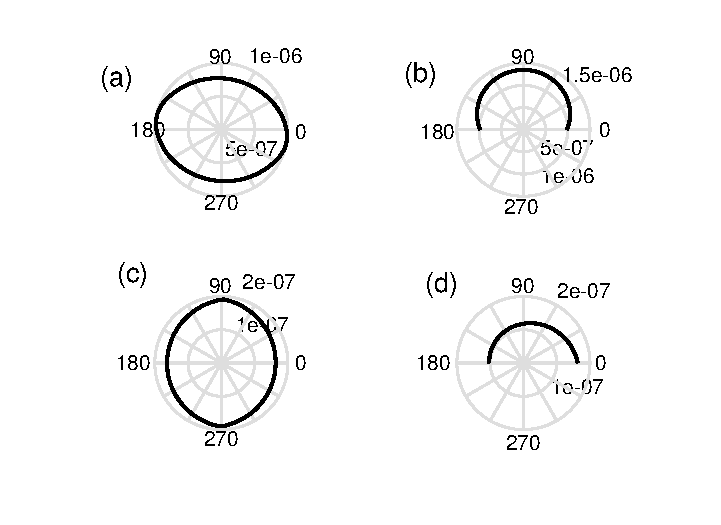
\includegraphics[width=10cm,height=5.3cm]{figures/GC_beamforming/polar1.eps}  
\vspace{-8mm} 
 \caption{\label{fig:polar} Directivity of received signal before (a,b) \& after (c,d) beamforming}
 \vspace{-7mm} 
\end{figure}
  
Note that the maximum transmission power $P^{max}_i$ is limited by the permitted level of signal propagation through tissues as $P_i\leq P_S$. If there are multiple concurrent transmissions, then the cumulative signal at any point should also meet the safety criteria $\sum_{i=0}^{M-1} P_i\leq P_S$. Thus, for safe and energy efficient choice of transmit power, the safety weight is chosen as:
\begin{equation} \label{e:ws}
w_{ij}^s = max\left( \frac{\delta_{jc}^{M-x}}{\hat{\delta}_{j}^{M-x}},\frac{\sum_{i=0}^{M-1} P_i}{P_S} \right),
\end{equation}
$\forall i\in\{1,..,M\}\  \&\  \forall j\in\{1,..,M\} + \{R\}$. Using $w_{ij}^s$, the magnitude of $P_i$ can be estimated using (\ref{eqn:Pi}).
 
\noindent$\bullet$ \textbf{Phase-match weight ($w_{ij}^p$):} As seen in Fig.~\ref{fig:multi}(c), the mismatch in phase among the signals results in destructive signal combination, and thus, reduces the net received power. To perfectly synchronize the uniformly distributed planar implant array, we first match the link-dependent phase shift of each implant obtained in (\ref{e:psi}) with respect to the reference position at ($O$). Then, using the good cross-correlation property of the Gold codes that we use later in Sec.~\ref{sec:cs}, we extract the phase differences from the frequency offsets iteratively as $\gamma' h_{iR}^{M-S}$ and compute the overall phase lag of each implant in the form of Phase match weight as: 
\begin{equation}\label{e:wp}
w_{ij}^p=\psi h_{iR}^{M-S}+\gamma' h_{iR}^{M-S} 
\end{equation}

 \begin{figure*}[t]
	\centering
	%\vspace{-2mm}  %
	\includegraphics[width=17cm]{figures/GC_beamforming/blockDiag.pdf} 
	\caption{\label{fig:spreading} CDMA \& beamforming based MAC framework for implants communication using GC-IBN}
\end{figure*}

\noindent$\bullet$ \textbf{Steering weight ($w^t$):}
This weight allows steering the signal from the transmitter to the relay with the desired beam shape given in Fig.~\ref{fig:polar}.(c)-(d). In the desired beam, along the elevation plane in Fig.~\ref{fig:polar}.(d), the beam power is increased at $\phi$=$0$ towards the position of the relay and in the azimuth plane in Fig.~\ref{fig:polar}.(c), the propagation is steered away from the neighbors at $\theta$=$0,\pi$. The corresponding steering weight is given as: 
\begin{equation} \label{e:wt}
w^{t}_{iR}= sin(k\theta_{iR})cos(k\phi_{iR})+sin(k\theta_{iR})sin(k\phi_{iR})
\end{equation}
where, $\theta_{iR}$ and $\phi_{iR}$ are the respective relative azimuth and elevation angles, respectively, between the implant and relay (refer Fig.\ref{fig:angles}), $k=\frac{2\pi f}{c'}$ is the wave number, $c'$ is the propagation speed of signal through the tissue medium estimated using the permittivity of the medium as,
\begin{equation}
c' = c/\sqrt{\epsilon}\,\, m/s
\end{equation}
where $c$ is propagation speed of light in vacuum and $\epsilon$ is the permittivity of the medium. $c'$ for muscle is around $9.5e6\ m/s$ and that of skin is around $8.3e6\ m/s$.

We adjust the array factor of the $\overrightarrow{H}$ field in (\ref{e:Harray}) using the three weights derived above as, 
\begin{equation}\label{e:AFnew}
E[AF_H]\text{=}\frac{1}{M}\sum_{i=0}^{M-1} \frac{1}{w_{iR}^s} \overrightarrow{H_i}gh_{iR}^{M\text{-}S} e^{j\omega \left(\psi_{iR}^{M\text{-}S}+\gamma_{iR}^{M\text{-}S} \right)} e^{w^{t}_{iR} - w_{iR}^p}
\end{equation}

%\noindent \textbf{Average power pattern \& energy efficiency:}
The average power pattern of the uniformly distributed planar array can be estimated as $E[|AF|] = |AF|(1-\frac{1}{M})+\frac{1}{M}$. 
We use our simulation environment to study the maximum power level in the tissue area using 
\begin{equation}\label{e:Pmax}
P^{max}=max_{\{r,\theta,\phi\}}  E[|AF|]
\end{equation}

\section{Hardware Implementation with Tissue Phantom}
\label{sec:implement}
In this section we implement near-field beamforming developed in section \ref{sec:bf}. We describe the testbed and present the results that quantify the effects of beamforming. 
\subsection{Experimental Setup}

We design a testbed using two USRP X310 software defined radios (SDRs), one each at the transmitter and receiver ends. Two distinct transmitters are installed on the same X310, since the SDR supports up to two LFTX daughter-boards. These low frequency daughterboards are set to 400 KHz center-frequency, which is within the range for galvanic coupling previously identified in~\cite{tbiocas}. Similarly, a LFRX daughter-board is used on the receiving X310. We implement near-field beamforming using the phase-match and steering weights analyzed and calculated in Sec. \ref{sec:bf}. The physical system layout and block diagram are given in Fig~\ref{F:testbed}. We transmit QPSK modulated signals from two transmitters, A \& B simultaneously, with limits on the transmit power to ensure it complies with the ICNIRP rules mentioned in Sec. \ref{sec:exp}.
The SDRs are configured and programmed in MATLAB utilizing the wireless communications toolbox functions.
In order to ensure that there is no ground coupling between the transmitters and the receiver, the receiver is connected to a battery source. All SDRs are given the same external clock inputs through the  OctoClock, also from National Instruments, to ensure synchronization.

\begin{figure*}[h!]
\centering

    \begin{subfigure}[b]{0.35\textwidth}
        \centering
        \includegraphics[width=0.95\linewidth]{figures/GC_beamforming/testbed_labels.jpg}
        %\caption{Physical experimental testbed} 
        \label{F:testbed}
    \end{subfigure}%
    \begin{subfigure}[b]{0.6\textwidth}
        \centering
        \includegraphics[width=0.95\linewidth]{figures/GC_beamforming/testbed_schem.pdf}
        \label{F:testbed}
    \end{subfigure}
    \caption{Photo and diagram of the testbed}
    \label{F:testbed}
\end{figure*}


For the purpose of this testbed, the same data is generated and sent from the two transmitters to ensure a common bit-stream for beamforming. 
Each data set, after modulation, is multiplied by a phase offset to apply its beam weight and achieve constructive interference.
The beam weights for each transmitter is calculated using equations \ref{e:wp} and \ref{e:wt}. The weights are then summed together and applied to the transmitted signal as per (\ref{e:AFnew}). The phase match weight  ($w^p$) is a sum of the phase offset induced by the channel and modeled in \cite{tbiocas} and the frequency offset of the cross-layer path from muscle to fat to skin (M-S).
Even though the entire system is connected on a common 10 MHz clock ensuring hardware frequency synchronization, we note there exists a constant frequency offset, possibly that of the cross-layer path. In our experimental setup we compensated for this effect in the receiver using a MATLAB coarse frequency compensator function. The steering weights ($w^t$) are calculated using the physical distances of the transmitters, from each other and from the receiver.

The transmitting electrodes are placed on the muscle layer. The beam-formed GC signal is received by the receiving electrodes that are placed on the skin layer, acting as the relay node. In the following subsection, we present the results of the received signal strength measurements and BER.

\subsection{Experimental Results}
There is an increase in received signal power when the two transmitters' weights are phase matched. As seen in Fig. \ref{fig:RSSI}, there is an increase of 3 dB in the received power when the two transmitters are in phase from the lowest received power achieved using TX A.
This result matches the theoretical expected doubling in received power with two transmitters. We notice a 1 dB difference between the individual transmissions of the two TXs (A and B). This difference can be attributed in the different paths between each transmitter and the receiver pair.

The phase offset steering weights are calculated based on the position of the transmitters and receiver, thickness of tissue phantom, using (\ref{e:wt}). The steering weight is summed with the phase match weight and is introduced to the transmitter as a phase offset to TX B. However, during experimentation we discovered a range of phase offsets for which the highest received power did not change significantly (more than 0.4 dB). In order to investigate the effect of the phase offset on the received signal strength for a wide range of phase angles, we performed an angle sweep keeping the phase offset of TX A at \ang{0} and varied the phase offset of TX B from \ang{1} to \ang{360}. As the results in Fig. \ref{fig:anglesweep} show, the maximum received power occurs at \ang{87}, whereas for the same setup the theoretical optimal phase offset should be \ang{62}, neglecting the frequency offset $\gamma' h_{iR}^{M-S} $ of equation (\ref{e:wp}). That offset is neglected because of the frequency compensation of our system. We notice that the received signal strength from \ang{60} to \ang{110} does not increase by more than 0.4 dB, ensuring that the constructive interference occurs for a range of approximately \ang{50}. The destructive interference has its lowest point at \ang{270}.

 \begin{figure}[t]
	\centering
	%\vspace{-2mm}  %
	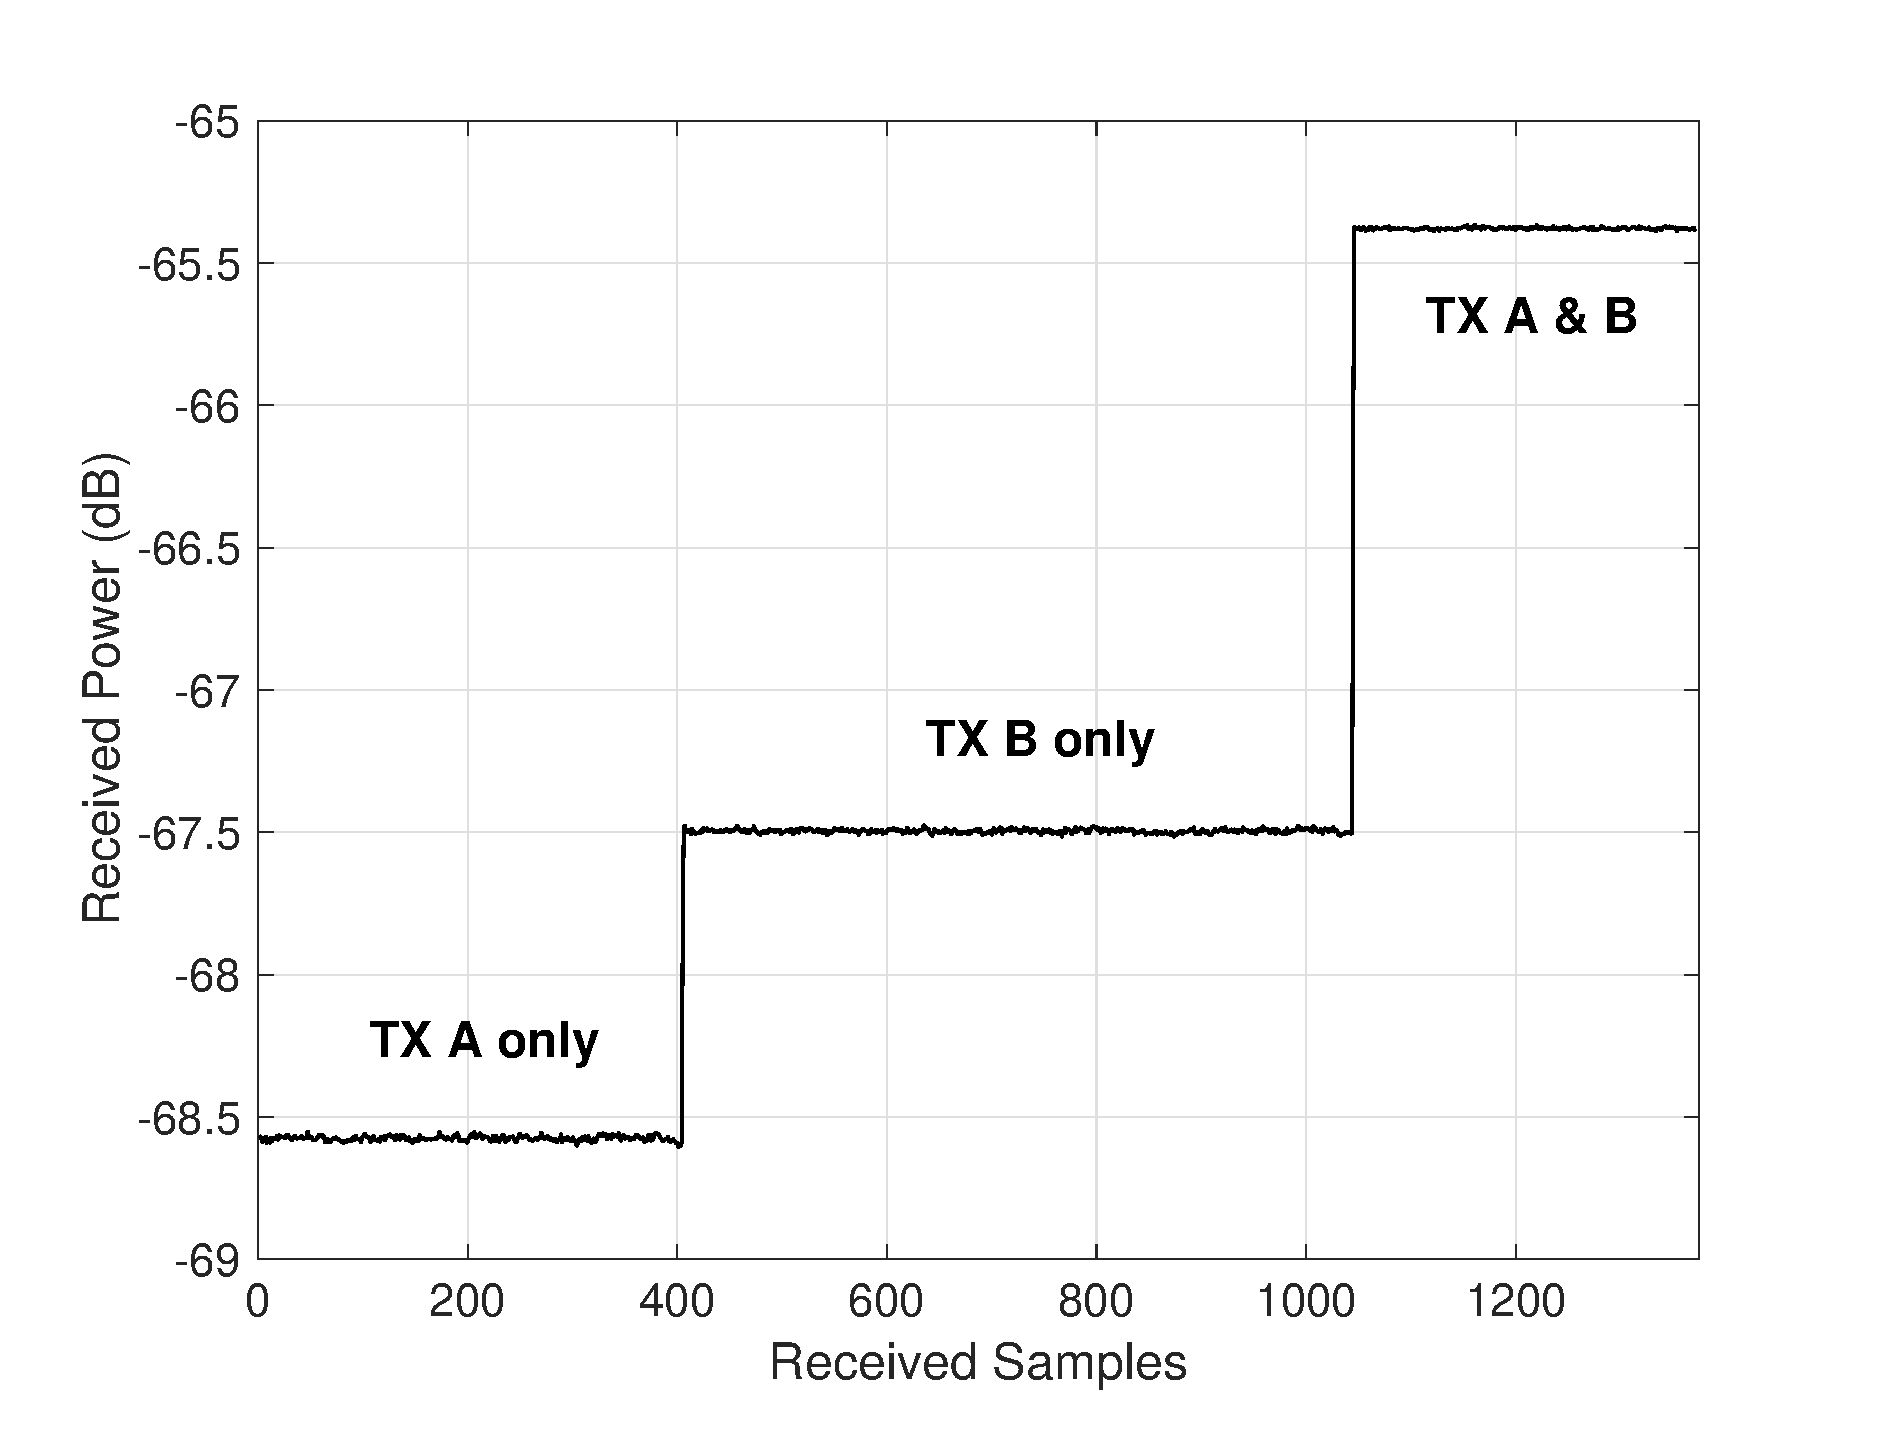
\includegraphics[width=0.7\textwidth]{figures/GC_beamforming//RSSI_curve_80.eps} 
	%\vspace{-3mm}
	\caption{\label{fig:RSSI} Received Signal Strength of three configurations (Tx A only, Tx B only and Tx A \& B) with phase match weights} \vspace{-2mm}
\vspace{-3mm}
\end{figure}

 \begin{figure}[t]
    \centering
	%\vspace{-2mm}  %
	\includegraphics[width=0.7\textwidth]{figures/GC_beamforming/BER_plot_finall.pdf} 
	%\vspace{-3mm}
	\caption{\label{fig:BER} Average BER measurements for 4 configurations (Tx A only, Tx B only, Tx A and B with phase match weights, Tx A and B without phase match weights) }
\vspace{-3mm}
\end{figure}

\begin{figure*}[t!]
\centering

    \begin{subfigure}[b]{0.5\textwidth}
        \centering
        \includegraphics[width=0.95\linewidth]{figures/GC_beamforming/comsol_nobf.png}{a}
        \caption{Logarithmic current density without beamforming} 
        \label{F:nobeamf}
    \end{subfigure}%
    ~
    \begin{subfigure}[b]{0.5\textwidth}
        \centering
        \includegraphics[width=0.95\linewidth]{figures/GC_beamforming/comsol_bf.png}{b}
        \caption{Logarithmic current density with beamforming}
        \label{F:beamf}
    \end{subfigure}
    \caption{COMSOL\textsuperscript{\textregistered} simulations for current density throughout phantom tissue}
    \label{F:comsol}
\end{figure*}

We also simulated the behavior of our setup using the finite element analysis COMSOL software, to measure current density at various points of the skin layer. As seen in Fig. \ref{F:comsol}, when the beamforming weights are applied to the two transmitters, there is higher current density at the receiver. These simulations prove that applying beamforming within our system effectively combines the power of several implants and increases the system efficiency.

Our testbed is designed to study intra-body communication as a whole, by providing insights on the communications front of implanted sensors transmitting measurements to a receiving on-skin relay. For this reason, the decoding capabilities of the system are of great interest. With an increase in received signal strength, and therefore SNR, the BER of the system when beamforming is enabled is lower than that of individual transmissions. As seen in Fig. \ref{fig:BER}, the BER of the system when both transmitters are transmitting with beamforming falls in the order of $4e$-$4$, compared to $2e$-$3$ for the scenario with no beamforming. This proves that an implant network where multiple sensors transmit with matched phases resulting in constructive beamforming results in a system with better decoding capabilities. We performed experiments for both wet and dry conditions and it can be seen that the wet conditions lead to a lower BER overall since the received signal strength improves through wet tissue. The received signal strength of our system does not exceed 0.31 $ \mu W$, which is below the mW range provided in \cite{ICNIRP}, while we also monitor the TX power to ensure safe transmissions.
 \begin{figure}[t]
	\centering
	%\vspace{-2mm}  %
	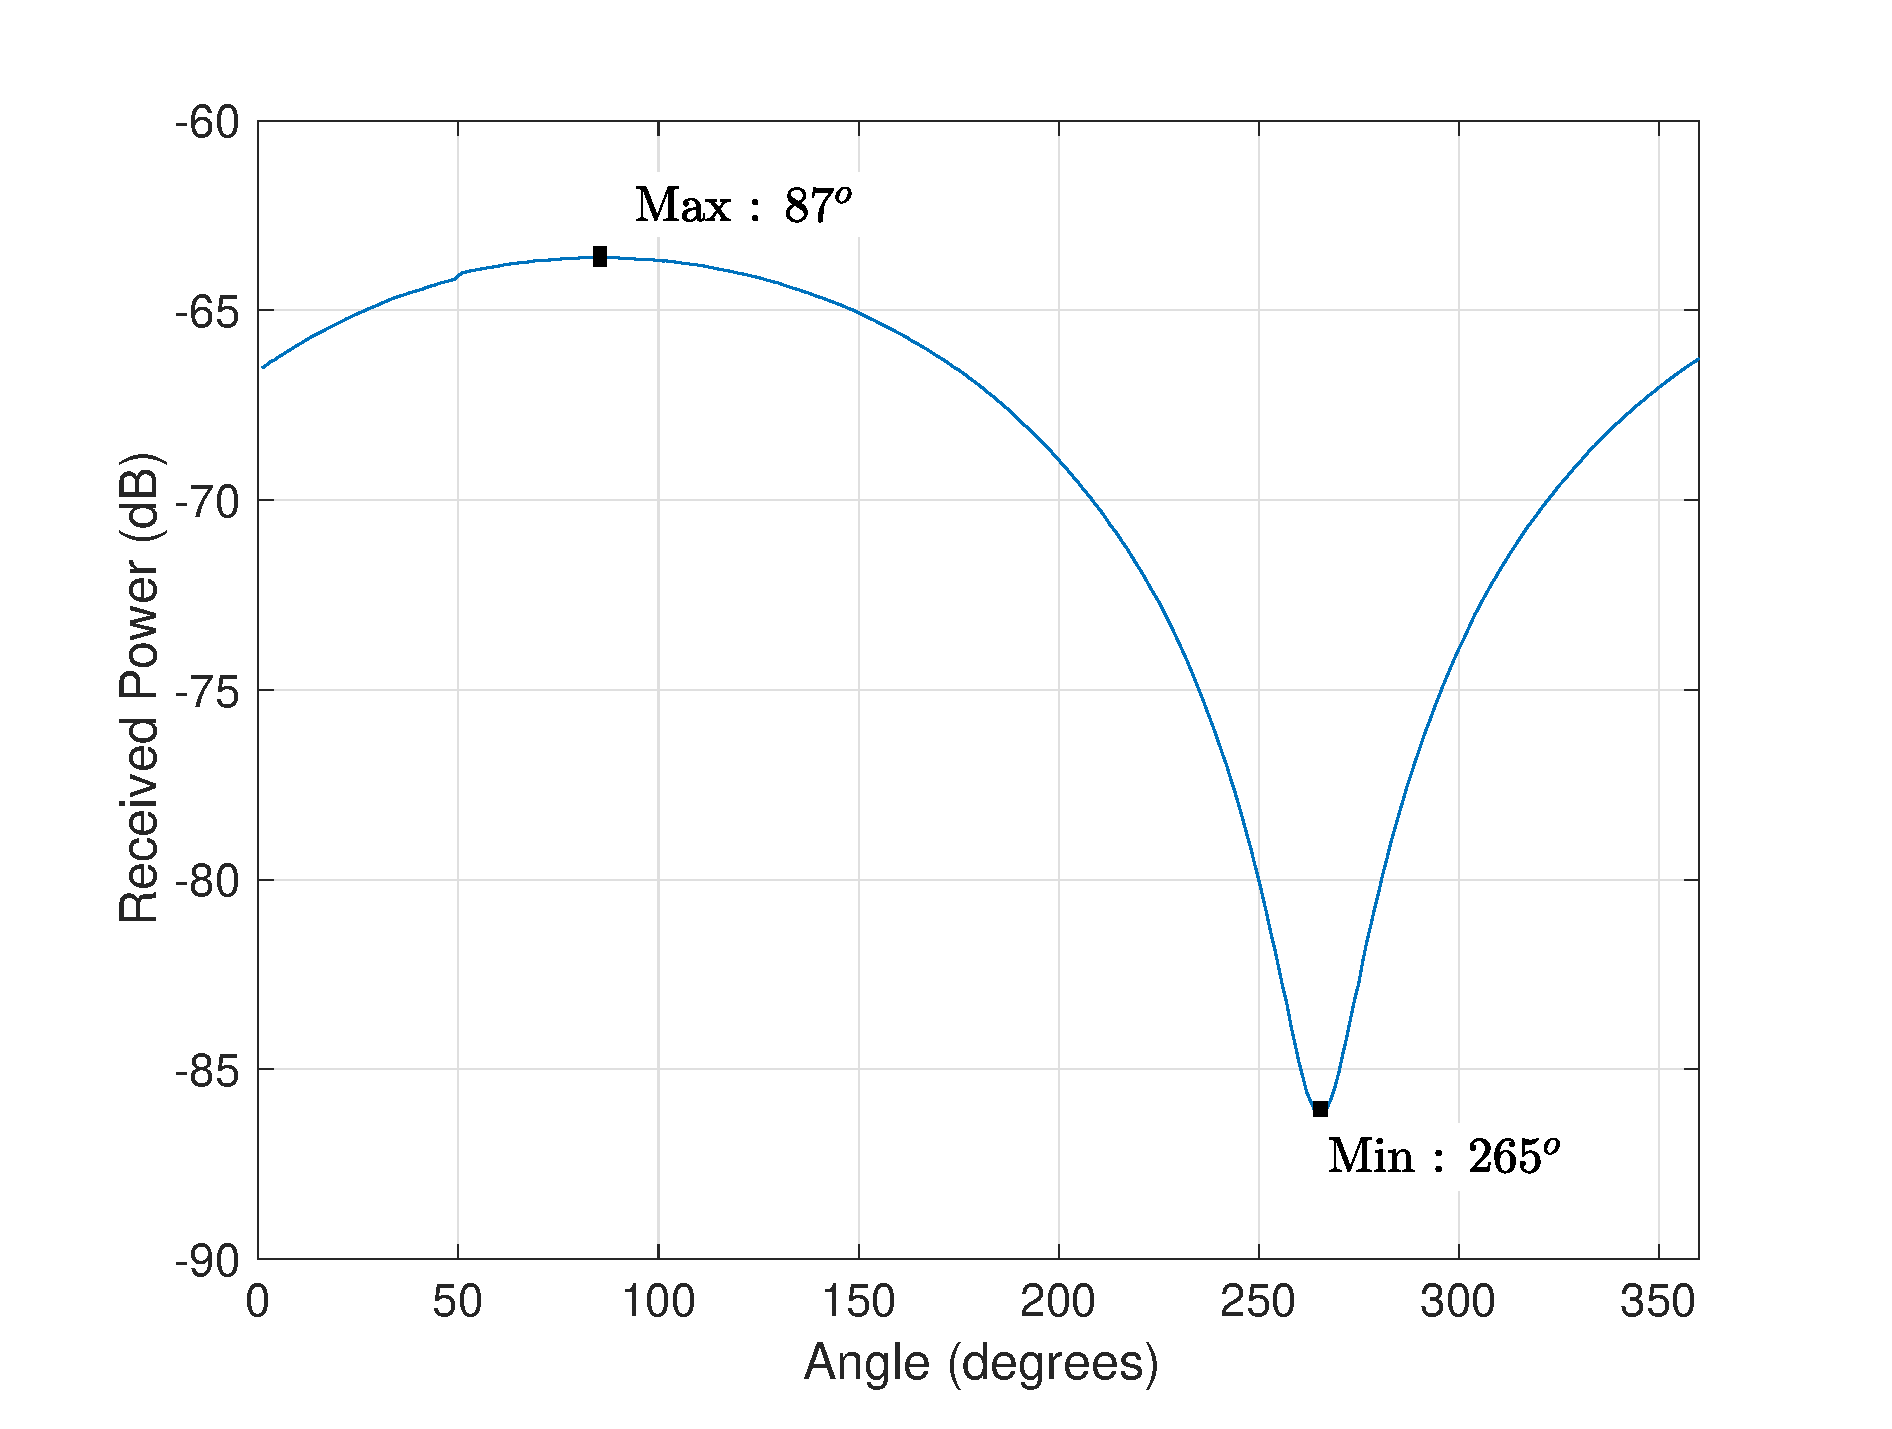
\includegraphics[width=0.95\linewidth]{figures/GC_beamforming/angle_sweep_fig.eps} 
	%\vspace{-3mm}
	\caption{\label{fig:anglesweep} Received Signal Strength with two transmitters, changing the angle of Tx B from 0-360 degrees} \vspace{-2mm}
\vspace{-3mm}
\end{figure}


\section{Beamforming using joint Compressive Sensing-CDMA} 
\label{sec:cs}
Implants participating in distributed beamforming fashion must transmit a common data vector to the on-skin relay. We propose a CDMA procedure to share data among the implants before initiating the beamforming process.
Specifically, we develop a compressive sensing (CS) transmission technique to reduce the number of measurements to send, which further results in lowering the transmission time and energy.	
The beam formation and the process of end-to-end data communication is split into five stages, as described below (see Fig.~\ref{fig:flowchart}):

\noindent $\bullet$ \textbf{Stage I. Resource assignment by the relay:} Each communication cycle starts a parameter setting beacon by the relay that allows implants to synchronize, set duty cycles for peerlevel and beamforming-based communication, use CDMA codes to partition the collision domain, and compute feedback weights for the array factor given in (11), (12) and (13) for optimal beamshaping (refer to stage.1 in Fig.10). Communication from implants are acknowledged in a successive round, enabling the implants to sleep immediately after they transmit the beam. Specifically, the parameters setting includes a synchronization message that delivers the information about two synchronization time slots. In the first time slot window the implants are allowed to send their data to a peer aggregator, while during the second time slot all the implants listen for the collected data that the aggregator is sending back to them. At the end of the second time slot, each implant sends such common data to the relay on the surface acting as distributed beamforming. Such procedure is required since we need each implant to have a common data vector prior to beamforming, thus the relay also appoints an aggregator (IDA) for the communication round. The aggregator’s role is simply to collect the individual and simultaneously transmitted spreaded sequences that combine in the tissue channel, and save this as the common data vector. The aggregator is a peer-implant, and its role is rotated in every round. Note that only a coarse synchronization is required during peer communication phase as specified at Stage III: an implant can choose to transmit anytime within the allowed window. For this purpose, quasi-orthogonal CDMA Gold codes are chosen for their good performance in an asynchronous CDMA transmissions.

%Before the implants share their data through the CDMA scheme, a precoding CS scheme is employed at each implant in order to send less samples of data
Specifically, a joint CS-CDMA scheme is proposed where the Gold codes are multiplied by the CS coding matrix. This way, the implants send less samples of data to further save energy while exploiting the possibility of fast simultaneous transmissions. Both the decoding and decompression of data are performed only at the on-skin relay, so that the implants do not have to perform any complex tasks.

\noindent $\bullet$ \textbf{Stage II. CS downsampling of data transmission:}
CS theory allows to reconstruct a signal with much lower samples than its dimension, provided that signal is sparse in some basis \cite{CDSP} and restricted isometric property (RIP) is satisfied \cite{candes} \cite{Vizziello}. Following this reasoning, implants may send a lower amount of sensed data reducing the energy consumption, one of the main concern in intra-body networks.\\
In practical applications, implants may not transmit data continuously. Hence, we assume that the sensed data is sparse, i.e., the implant activity is sporadic and i.i.d with probability $p_a\ll 1$ in the considered time window.
Thus, the sensed data $\mathbf{b}_i$ of size $U \times 1$ at implant $m_i$ may be 
represented as a linear measurement $\mathbf{x}_i$ of size $N \times 1$ with $N\ll U$ as
\begin{equation}
{\mathbf{x}_i=\mathbf{F}_i \mathbf{b}_i}
\label{eqCS}
\end{equation}
that corresponds to CS coding matrix multiplication block in the left side of Fig. \ref{fig:spreading}, where measurement vector $\mathbf{x}_i$ is a compressed version of $\mathbf{b}_i$ obtained through the CS coding matrix $\mathbf{F}_i$, i. e., the dictionary, with
\begin{equation}
\mathbf{F}_i=\mathbf{Q}_i \mathbf{\tilde{F}}_i 
\label{eqCDMA2}
\end{equation}
where the elements of $\mathbf{\tilde{F}}_i$ are taken from Rademacher distribution and $\mathbf{Q}_i$ is the discrete Fourier transform (DFT) matrix. 
Note that  $ \mathbf{b}_i \in \mathcal{B}_{a}$, where $\mathcal{B}_{a}$ is the discrete alphabet $\mathcal{B}$ augmented to represent also the inactivity. Specifically, an inactive implant is equivalent to transmit symbol $0$ while  activity corresponds to data modulated according to the alphabet $\mathcal{B}$ \cite{Dekorsy12}.\\ 
The size of the compressed data $\mathbf{x}_i$ that implant $m_i$ shares through the CDMA procedure is much lower than the original $\mathbf{b}_i$.
Moreover, since the transmission for some health applications is sporadic and also short, we can interpret it as  group sporadic transmission, which allows to develop a faster CS algorithm as detailed in Stage V.

\noindent $\bullet$ \textbf{Stage III. Peer communication phase:} The relay provides a time window ($T_B$) for all implants to combine their data using the Gold codes and transmit them simultaneously. 
Note that an implant can opt out of transmission in a cycle and sleep for prolonged period if its sensing cycle is longer. Also, the communication is not strictly synchronized that relieves the implants from complex scheduling and mutual phase offset computation for this first round of messaging. An implant can choose to transmit anytime between the allowed window of peer-level communication.
This transmission is intentionally set to very low power given that it traverses the high-gain M-M path to the aggregator node (refer to stage.2 in Fig.\ref{fig:flowchart}).The spreading factor $L$ of the Gold code is chosen based on the number of implants. The implant ID is associated with a unique spreading code sequence $\mathbf{c}_i$ within the CDMA codebook.\\ 
For $N$ compressed data bits $\mathbf{x}_i$ of the implant $i$, each
bit is directly multiplied by the Gold code $\mathbf{c}_i$ with $L$ elements to generate the spread sequence $x_{i,n}\mathbf{c}_i,\ \forall \ i\in\{1,..,M\},\  n\in\{1,..,N\}$ of size $L\times 1$ (refer to the Gold code generator multiplication in  Fig. \ref{fig:spreading}). These quasi-orthogonal Gold codes have good cross correlation properties that enable simultaneous almost non-interfering transmissions. After spreading at the sampling time instant corresponding to the index $k,\ \forall k \in \{0,..,L-1\}$, the implants transmit the spreaded sequence $x_i\mathbf{c}_i$ through the M-M path. At this stage, neither other implants nor the aggregator performs any decoding. 

 
At $n$-th bit time instant, the aggregator receives the sequence $\mathbf{d}_n$ as a vector of size $L \times 1$ from the $M-1$ implants as,
\begin{equation}
	\mathbf{d}_n = \sum_{i=1}^{M-1} g_{iA}^{(M-M)} x_{i,n} \mathbf{c}_i  + \mathbf{w} 
	\label{eqCDMA0}
\end{equation}

where $A$ represents the aggregator, $x_{i,n}$ is the $n$-th bit sent by the implant $m_i$ after applying CS,  $\mathbf{c}_i=[c_i(0), c_i(1),..., c_i(L-1)]^T$ is the spreading code for implant $m_i$ with $x_{i,n} \mathbf{c}_i$ expressed in antipodal form, $()^T$ denotes the transpose, and 
$\mathbf{w}$ is the iid additive white Gaussian noise vector with zero mean and variance $\sigma^2$ of size $L \times 1$ given by $[w(k-L+1), w(k-L+2),..., w(k)]^T$. Since each implant transmits in a narrow band channel ($400\ kHz$) the M-M channel can be represented as a single tap channel \cite{tbiocas}. We assume that $g_{ij}^{(M-M)}$ is constant during a transmission cycle. 

The final vector $\mathbf{d}$ of size $LN \times 1$ is given by
\begin{equation}
	\mathbf{d} = [\mathbf{d}_1 \phantom{x} \mathbf{d}_2 \phantom{x} ... \phantom{x} \mathbf{d}_n \phantom{x} ... \phantom{x} \mathbf{d}_N] 
	\label{eqCDMAd}
	\end{equation}
Eq. (\ref{eqCS})-(\ref{eqCDMAd}) summarize the joint CS-CDMA procedure for data transmission, showing that the sent data $\mathbf{d}$ is given by the original bits $\mathbf{b}_i$ for each implant $m_i$ in (\ref{eqCS}) multiplied by a combination of CS coding matrix $\mathbf{F}_i$ and Gold codes $\mathbf{c}_i$.\\
 
Once the aggregator receives the overall CDMA vector containing the spread data $\mathbf{d}$, it sends back the common CDMA vector $\mathbf{d}$ representing the aggregated value to the peer implants through a single broadcast, again using the high-gain M-M path. 

The spread data received back at the $m_i$-th implant can be expressed as
\begin{equation}
\tilde{\mathbf{d}}_i=g_{Ai}^{(M-M)}\mathbf{d} + \mathbf{w}
\label{eqCDMA2b}
\end{equation}
Now, all the implants have the common CDMA vector (refer to $\tilde{\mathbf{d}}$ in Fig. \ref{fig:spreading}), which may only slightly differ from each other depending on the channel coefficient of the M-M path from the aggregator to the specific implant according to (\ref{eqCDMA2b}).
  
\begin{figure}
 \centering
% \vspace{-2mm}  %
\includegraphics[width=8cm,height=11cm]{figures/GC_beamforming/diagram.pdf}  
\vspace{-2mm} 
 \caption{\label{fig:flowchart} Stages showing the entire end-to-end implant to relay communication}
 \vspace{-6mm}
\end{figure}
   
\noindent $\bullet$ \textbf{ Stage IV. M-S Beamforming phase:}
In this phase, each implant acts as an independent antenna array element and attempts to form a beam sending the same overall CDMA data vector that has been shared with all the implants at the instant $T_B$ predetermined by relay. The use of the same CDMA data during beamforming further improves the  SNR and lowers the required M-S transmission power at the implants as shown in Sec.\ref{sec:bf}. Although each implant acts as an element of a virtual antenna array sending the same information, the individual implant signals differ in amplitude and phase, as instructed by the beamforming weights. The implants tune their transmission based on the weights, such that all the transmissions from implants constructively amplify the received signal $\mathbf{y}$ at the relay and maximize the received power.

Thus, each implant sends the information at lower power compared to individual transmissions in the M-S channel, enabling significant energy savings.The received vector $\mathbf{y}$ at the relay (as shown in Fig. \ref{fig:spreading}) is given by
\begin{equation}
	\mathbf{y}=\sum_{i=0}^{M-1} S_{i} \tilde{\mathbf{d}}_i + \mathbf{w}
	\label{eqCDMA3}
\end{equation}
where $S_{i}$=$\frac{1}{w_{iR}^sM}gh_{iR}^{M\text{-}S}e^{j\omega\left(\psi_{iR}^{M\text{-}S}+\gamma_{iR}^{M\text{-}S} \right)} e^{w^{t}_{iR} - w_{iR}^p}$ obtained from (\ref{e:AFnew}) that accounts for both the steering coefficient of the implant $m_i$ and the channel coefficient of the M-S path from the implant implant $m_i$ to the relay $R$ on surface. The implants enter into the sleep state immediately after sending the beam until the next transmission cycle (see stage.3 in Fig.~\ref{fig:flowchart}).

\begin{figure*}[t]
 \centering
 \vspace{-2mm}  %
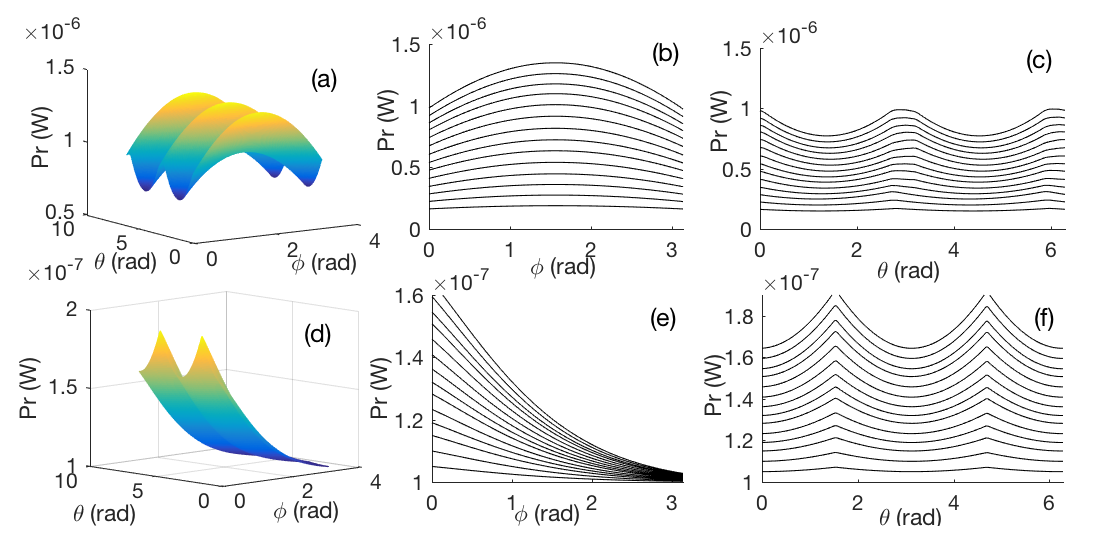
\includegraphics[width=17cm,height=6.5cm]{figures/GC_beamforming/multi.eps}  
 \caption{\label{fig:multi} Received power before and after beamforming}
 \vspace{-5mm}
  \end{figure*}
  
\noindent $\bullet$ \textbf{Stage V. Despreading, decoding and feedback at the relay:}

Having received the common CDMA vector through the beamformed signal, the relay performs despreading and CS data reconstruction using a matrix with the same Gold codes distributed to the individual implants and the CS coding matrices. In this way, it recovers the sensed data and the associated ID of each implant, as shown in the Relay block in Fig. \ref{fig:spreading}.\\ 

Going in more details, CS methods can be categorized broadly into accurate and stable convex relaxation iterative algorithms \cite{Donoho06}, \cite{Candes08}, and fast but less accurate greedy algorithms \cite{Masood13}, \cite{Dai09}. Since health applications require high reliability we focus on an accurate iterative solution. Specifically, as said before, in such applications the implant activity may be interpreted as group sporadic, thus we develop a group basic pursuit denoising (Group-BPDN) approach to reconstruct the sent data $\mathbf{b}_i$.
The  problem may be expressed as \cite{BergFriedlander:2008}
\begin{equation}
	\textrm{min} \    \  \sum_{v=1}^V\|\mathbf{b}_{i,v} \|_2   \ \textrm{  subject to } \|\mathbf{F}_i\mathbf{b}_i-\hat{\mathbf{x}}_{i} \|_2 \le \sigma
	\label{eqCSgroup}
\end{equation}
where the index $v$ refers to the group to which the data have been assigned, $\mathbf{F}_{i}$, $\mathbf{b}_{i}$, $\mathbf{x}_{i}$ are defined in (\ref{eqCS}), and $\sigma$ is the noise variance. The estimate  $\hat{\mathbf{x}}_{i} = [\hat{x}_{i,1} \phantom{x} \hat{x}_{i,2} \phantom{x} ... \phantom{x} \hat{x}_{i,n} \phantom{x} ... \phantom{x} \hat{x}_{i,N}]$ of size $N \times 1$ is obtained through the CDMA despreading that uses the cross-correlation of the received signal $\mathbf{y}$ in (\ref{eqCDMA3}) with the known Gold codes. 
Specifically, the element $\hat{x}_{i,n}$ of $\hat{\mathbf{x}}_{i}$ is calculated as
\begin{equation}
\hat{x}_{i,n}=\mathbf{y}^T_n\mathbf{c}_i
\label{eqCDMA4b}
\end{equation}
where $\mathbf{y}_n$ is the $L \times 1$ element of the $LN \times 1$ vector $\mathbf{y} = [\mathbf{y}_1 \phantom{x} \mathbf{y}_2 \phantom{x} ... \phantom{x} \mathbf{y}_n \phantom{x} ... \phantom{x} \mathbf{y}_N]$ and $()^T$ indicates the transpose.
\\
Note that the Group-BPDN minimizes quadratic
noise by solving the convex optimization
problem as a quadratic programming approach for which
efficient Interior-Point (IP) methods exist \cite{BergFriedlander:2008},
\cite{berg2}.


In terms of transmission and propagation time, the whole transmission cycle takes 
\begin{equation}\label{time}
4\displaystyle \frac{L}{\eta}\text{+} 2\frac{\psi x_{iR}^{M\text{-}M}+\gamma x_{iR}^{M\text{-}M}}{360 f}\text{+} 2\frac{\psi x_{iR}^{M\text{-}S}+\gamma x_{iR}^{M-S}}{360 f}\text{+}4T_R 
\end{equation} seconds, where $L$ is the frame (or chip) length and $T_R$ is the tissue relaxation time required between transmissions to assure normal tissue temperature under abnormal blood flow rates, calculated as $T_R= \sqrt{\frac{\epsilon}{\sigma}}$, $\epsilon\  \& \  \sigma$ being the tissue permittivity and conductivity.  

Finally the relay computes the weights $w^s_{iR}$,$w^p_{iR}$ and $w^t_{iR}$ using (\ref{e:ws}), (\ref{e:wp}) and (\ref{e:wt}) for the successive transmission and transmits them to the implants at the predetermined interval as given in the Beamforming weights block in Fig. \ref{fig:spreading} and in stage.1 in Fig.~\ref{fig:flowchart}.




\section{Performance Evaluation \& Results}\label{sec:results}   

In this section, we evaluate the energy savings achieved by the proposed CDMA based beamforming framework by (i) analyzing the proportion of energy propagating in the direction of the relay to that leaking in the undesired directions, (ii) studying the influence of the number of array elements on the implant power consumption, (iii) quantitatively measuring the improvement in implant lifetime, and (iv) comparing the energy consumption for the overall M-S path communication with/without our approach. We develop a 3-D multi-layer, heterogeneous tissue channel model in MATLAB, operating at a narrow band of $100\ kHz$. The tissue area has the dimension of $20\times 20 \mathrm{cm}$, with $r_{max}$=$20\ \mathrm{cm}$. The separation between the layer of implants in muscle and the surface is $2.2\ \mathrm{cm}$. The maximum safe transmit power is $1\ \mathrm{mW}$.

 \begin{figure}[b]
 \centering
\vspace{-6mm} 
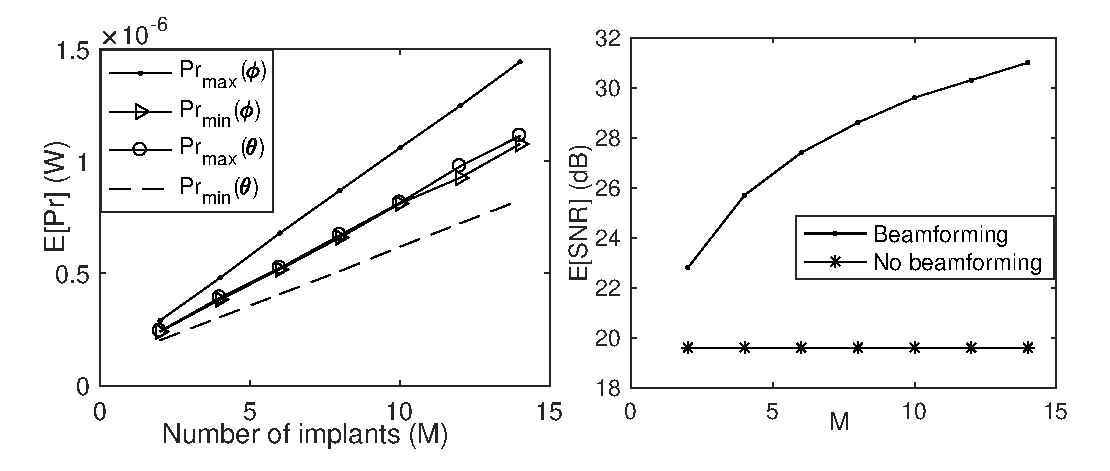
\includegraphics[width=0.95\textwidth]{figures/GC_beamforming/new2plots.eps} 
\vspace{2mm} 
 \caption{\label{fig:prplot} (a) Directionality (b) SNR before \& after beamforming} 
  \end{figure}
  
\subsection{Effectiveness of beamforming} The pattern of received power at the relay resulting from the sum of the signals concurrently propagating through the tissue medium without beamforming is shown in
Fig.~\ref{fig:multi}(a)-(c). Here, the propagation is oriented towards the longitudinal muscle direction (at $\phi$=$\frac{\pi}{2}$, $\theta$=$0,\pi$), where more energy flow occurs along the length of the arm. This causes minimal flux at the surface relay (at transverse direction at $\phi$=$0$). This pattern may also cause more interference to the potentially neighboring implants (refer Fig.~\ref{fig:expr}(left) for the direction of neighbors). Before beamforming, the ratio of energy flow in the required direction to undesired direction is $\approx 0.53$. Fig.~\ref{fig:multi}(d)-(f) shows the received signal at relay after beamforming, where more power is steered towards the relay (at $\phi$=$0$) and there is less power in the longitudinal direction ($\phi$=$\frac{\pi}{2}$, $\theta=0,\pi$) mitigating the interference to neighbors. 

Fig.~\ref{fig:multi}(b)-(c) shows power degradation when signals with different phases are combined together. After the phase mismatch is rectified using $W^p$ in the beamforming process, the signals add up constructively (refer Fig.~\ref{fig:multi}(e)-(f)) as demonstrated in Fig.~\ref{fig:expr}(d) and improve the received power by an additional $\approx 3\%$ as shown in Table.\ref{tab:result1} as $Pr(W^p)$. Note that this is the received power obtained after the transmit power is reduced to sufficient level using $w^s$ weight.
 We analyze the maximum induced power at every point in the given tissue area defined by $\theta$, $\phi$ and $r$ using (\ref{e:Pmax}) and verify that the cumulative received power at any point in the tissue with multiple concurrent transmissions does not exceed the restrictions posed by safety limits, confirming the tissue safety and normal thermal distributions~\cite{ICNIRP}. Using the simulation environment, we further ensure that $\int_{\theta} \int_{\phi} \int_{r} Pr dr d\phi d\theta \leq 25\ \frac{mA}{m^2}$. 

\noindent \textbf{Influence of number of implants:}
The resulting proportion of power in the required to undesired direction is plotted in Fig.~\ref{fig:prplot}.(a) illustrating that more power is steered towards the relay when there are more number of implants forming the array. Thus both the critical beamforming parameters namely, the per implant power conservation and the directivity of beamforming, are improved with the number of implants or array elements ($M$). The actual SNR for individual transmission from each implant through M-S path is compared with the exponential increase in SNR at the receiver after beamforming with $M$ implants in Fig.~\ref{fig:prplot}(b). 


\noindent \textbf{Implant lifetime:}
The transmission power of the implants is reduced to just meet the required SNR by applying the safe weight $w^s$ derived in (\ref{e:ws}). The resulting power consumed ($aPt$) in each implant vs $M$ and the corresponding improvement in implant lifetime is shown in Table.\ref{tab:result1}. %KRC- is the vs M or N? 
We see that the implant life dramatically extends from $10$ weeks when used without beamforming, to $\approx 138$ weeks with beamforming for the scenario with $14$ implants.	
  
\begin{figure}
	\centering
	%	\includegraphics[width=1\linewidth]{gbp_ber1.eps}
	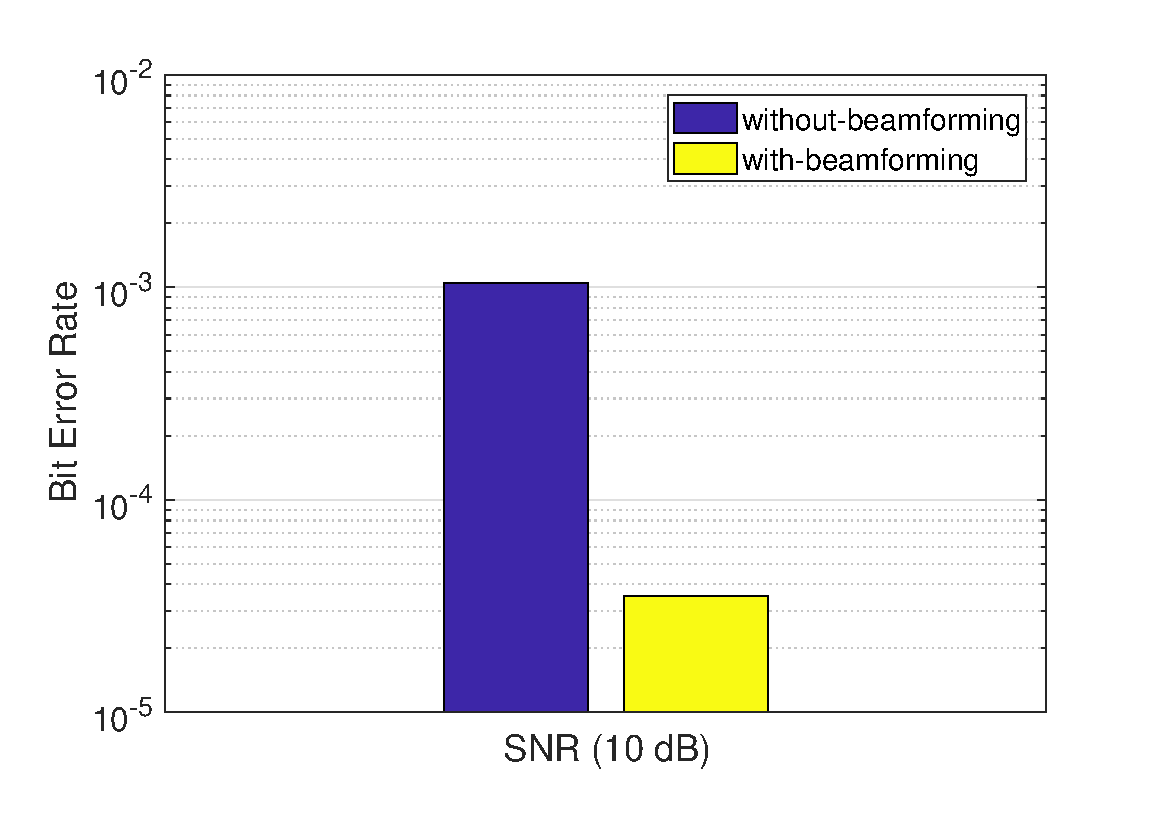
\includegraphics[width=10.5cm,height=7.5cm]{figures/GC_beamforming/sensor2delay2_beamforming_bar.eps}
	\caption{Bit error rate for CS-CDMA solution based on Group-BPDN and Gold codes with and without beamforming. Spreading sequence $L = 128$ chips, sparsity $= 40 \%$, maximum delay $= 2$ chip time duration, number of implants $M = 2$, data length $U = 5000$, compressed measurements $N = 2500$.}
	\label{Fig_result0}
	\vspace{-2mm}
\end{figure}

\begin{figure}[h!]
\centering
    \begin{subfigure}[b]{0.95\textwidth}
    	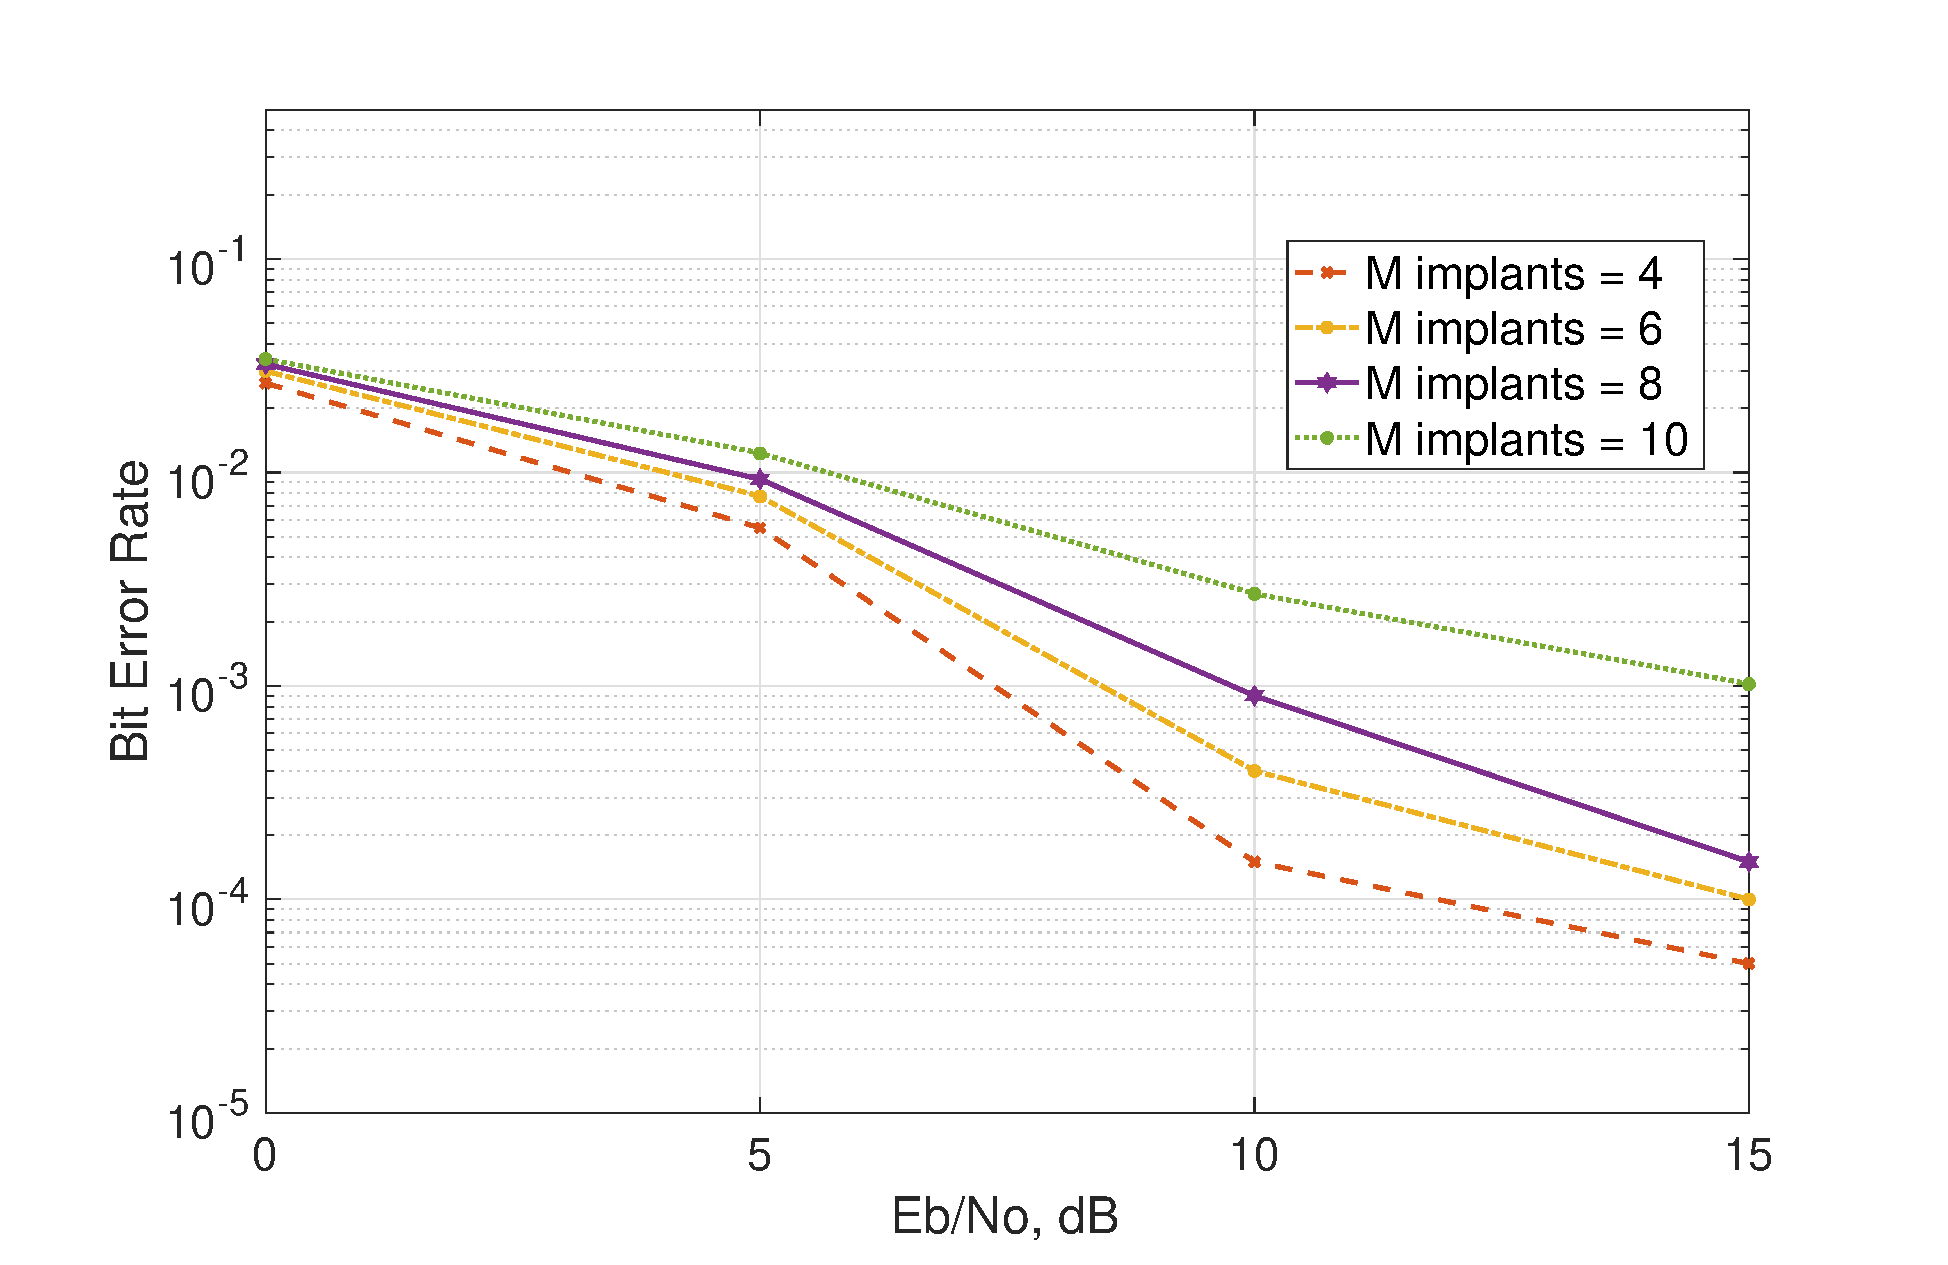
\includegraphics[width=\textwidth]{figures/GC_beamforming/ber_sensors_sp-40-delay_2.eps}
    	\caption{BER for CS-CDMA solution based on Group-BPDN and Gold codes, maximum delay $= 2$ chip time duration}
    	\label{Fig_result1}
    \end{subfigure}
    ~
    \begin{subfigure}[b]{0.95\textwidth}
	    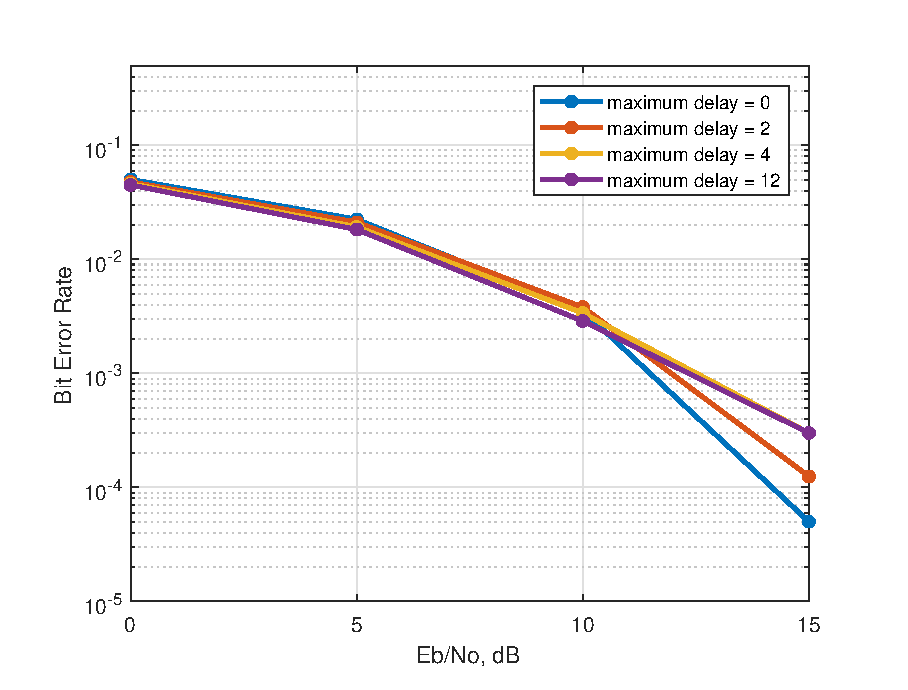
\includegraphics[width=\textwidth]{figures/GC_beamforming/delay_sp-40-sen-8.eps}
	    \caption{BER for CS-CDMA solution varying the max. delay (\# of chips) among implants' transmissions of the asynchronous scheme}
    	\label{Fig_result1bis}
    \end{subfigure}
    \caption{BER of CS-CDMA. Spreading sequence $L = 128$ chips, sparsity $= 40 \%$, data length $U = 5000$, compressed measurements $N = 2500$}
    \label{F:CSCDMABER}
    \vspace{-3mm}
\end{figure} 
  
\subsection{BER \& energy analysis for CS-CDMA beamforming}

The proposed CS-CDMA scheme allows concurrent transmissions for the implants which reduces the total time for data transmission. The implants perform only simple tasks to send the acquired data, while the burden despreading/decoding is carried out only at on-skin relay. Moreover, the CS procedure allows to further reduce the transmission time since a much lower number of samples are sent instead of the full senses data. There is, however, an additional overhead of (i) spreading the data using the Gold codes, and (ii) (albeit high gain M-M) communication between implants to the aggregator and back. We aim to study whether this cost is offset by the energy savings achieved by beamforming.

The proposed algorithm for asynchronous CS-CDMA recovers both the activity of the implants and their data in a certain time window.
The total number of sensors varies between $2$ and $10$. The spreading factor $L$ for the Gold codes is set equal to $128$ and the Group BPDN CS approach is used to recover data with different level of sparsity, which corresponds to the percentage of implant's activity in a certain time window.

Fig. \ref{Fig_result0} shows a comparison between the BER achieved by the proposed CS-CDMA solution with and without beamforming under the same parameter setting of the experimental setup in Sec. \ref{sec:implement}. Specifically two implants are considered and the BER improvement is due to SNR gain (2.5 dB) obtained when using beamforming.

The simulation results on Fig. \ref{Fig_result1} compare the achieved BER for different number of implants, describing that the system shows good performance with an increased number of implants. Fig. \ref{Fig_result1bis} illustrates the BER performance versus the maximum delay among the implant's transmissions. Each implant transmits with a random delay within the maximum one to simulate the asynchronous scheme in the peer communication phase inside the muscle. In low $E_b/N_0$ region the performance for different delays is comparable, while lower delays give better results when increasing $E_b/N_0$.

Fig. \ref{Fig_result2} focuses on the choice of the dictionary matrix $\mathbf{F}_i$ in (\ref{eqCDMA2}) for the proposed CS-CDMA algorithm. Indeed, the design of such matrix is one of the main concern in CS algorithms for an efficient solution. We compare the proposed $\mathbf{F}_i$ definition, based on DFT and rademacher distribution, with only DFT, and Gaussian and Bernoulli random matrix. The total amount of measurements has been fixed to $5000$ and results in Fig. \ref{Fig_result2} prove that the proposed solution shows high performance even when sending only $50 \%$ measurements, differently from DFT, Gaussian and Bernoulli matrices.

Fig. \ref{Fig_result3} compares the accuracy of the proposed CS-CDMA solution, based on Group-BPDN CS approach, with a modified version of it, i.e., when employing the greedy regularized group orthogonal matching pursuit (ReGOMP) algorithm. Fig. \ref{Fig_result3} shows that the proposed Group-BPDN based approach outperforms the ReGOMP solution for both values of sparsity ($20 \%$ and $40 \%$), showing high accuracy already when sending only $50 \%$ measurements. Note that for health applications the high accuracy is a stringent requirement.

\begin{figure}
	\centering
	%	\includegraphics[width=1\linewidth]{dict_angles.eps}
	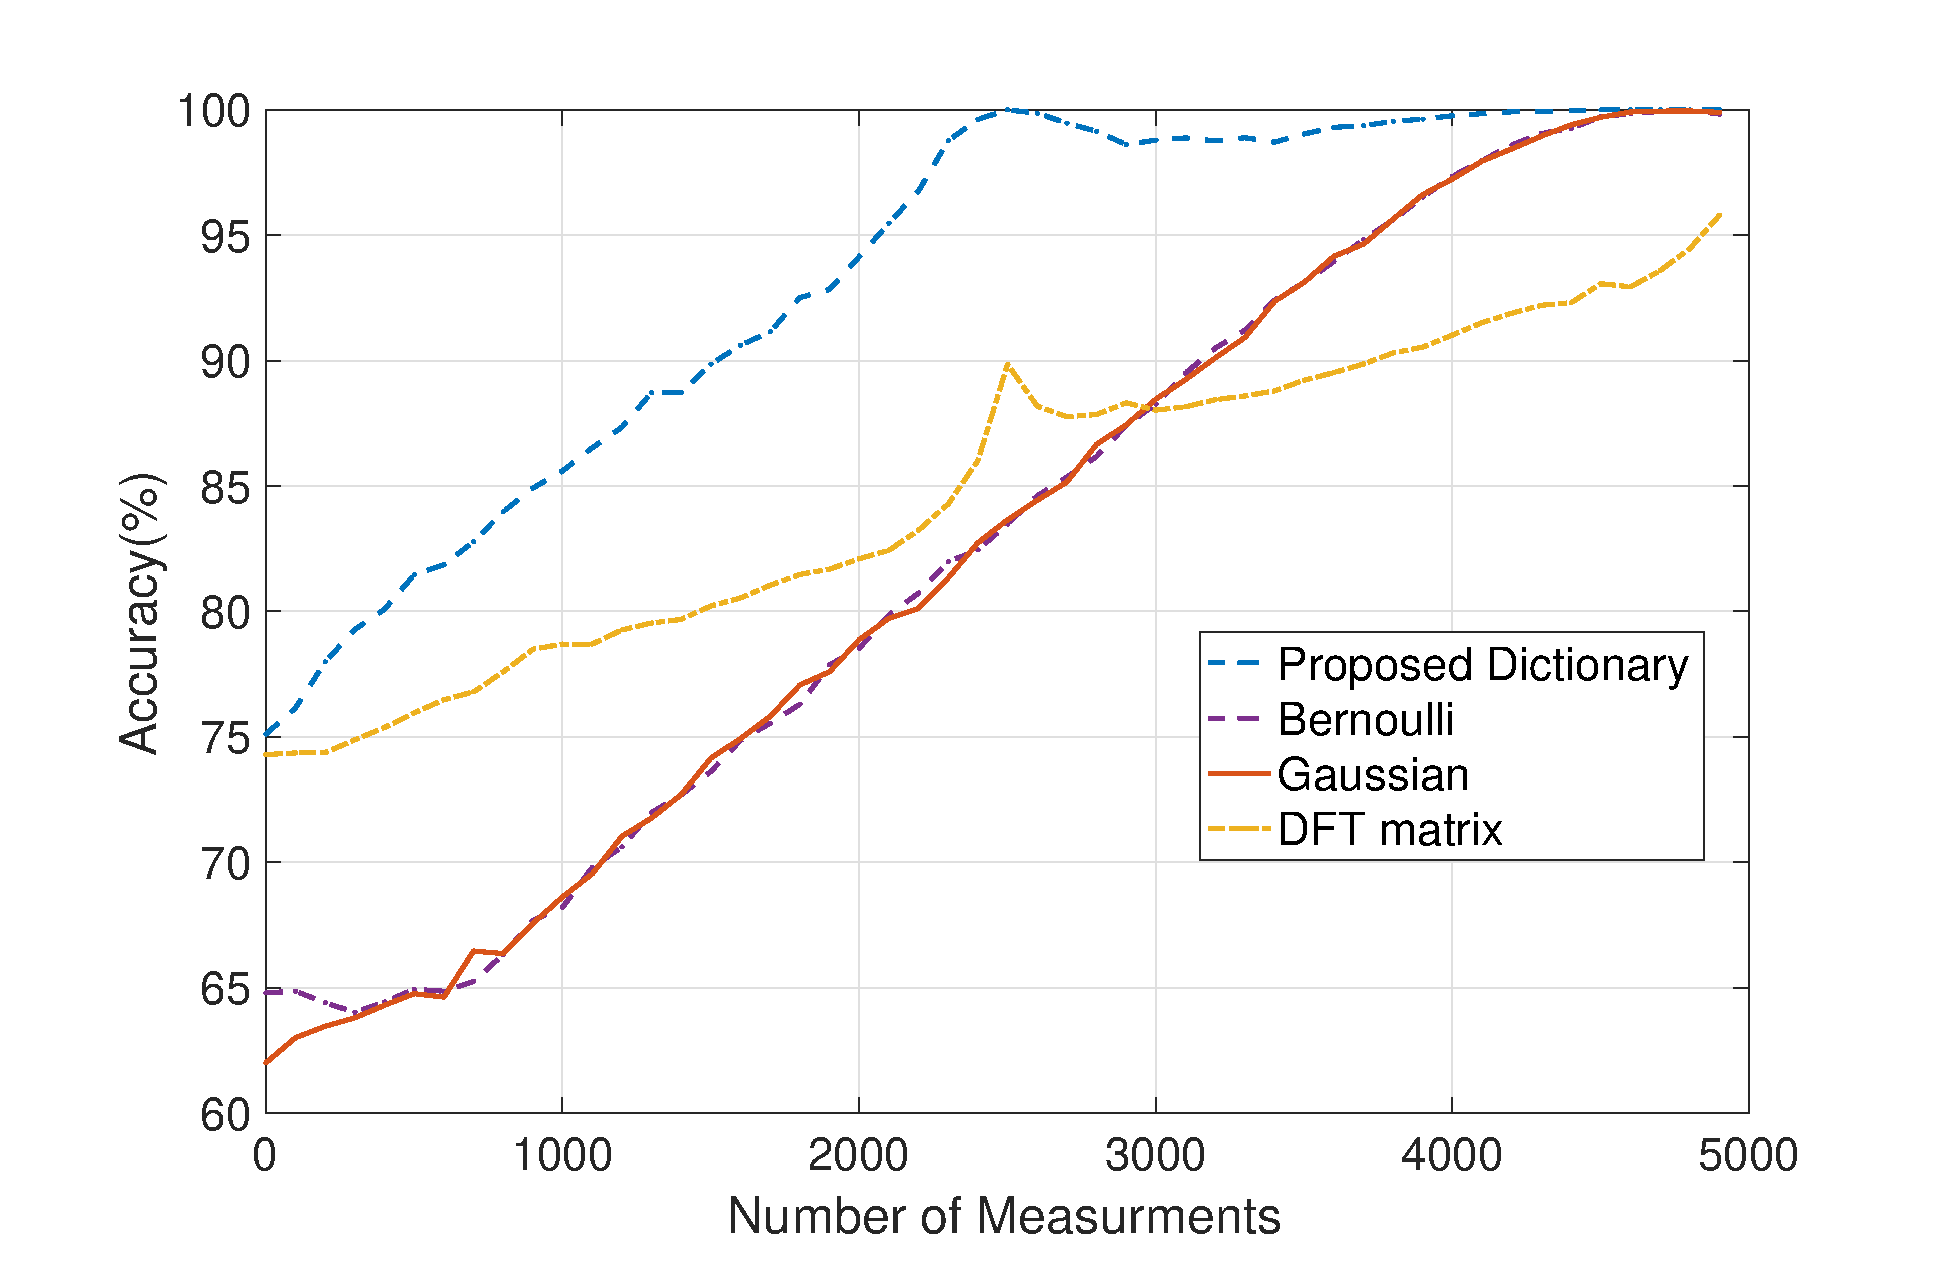
\includegraphics[width=0.95\textwidth]{figures/GC_beamforming/sen4sparsity-50-delay2-1.eps}
	\caption{Accuracy of the proposed CS-CDMA algorithm for different CS coding matrices.}	
	\label{Fig_result2}
\end{figure}
\begin{figure}
	\centering
	%	\includegraphics[width=1\linewidth]{dif.eps}
	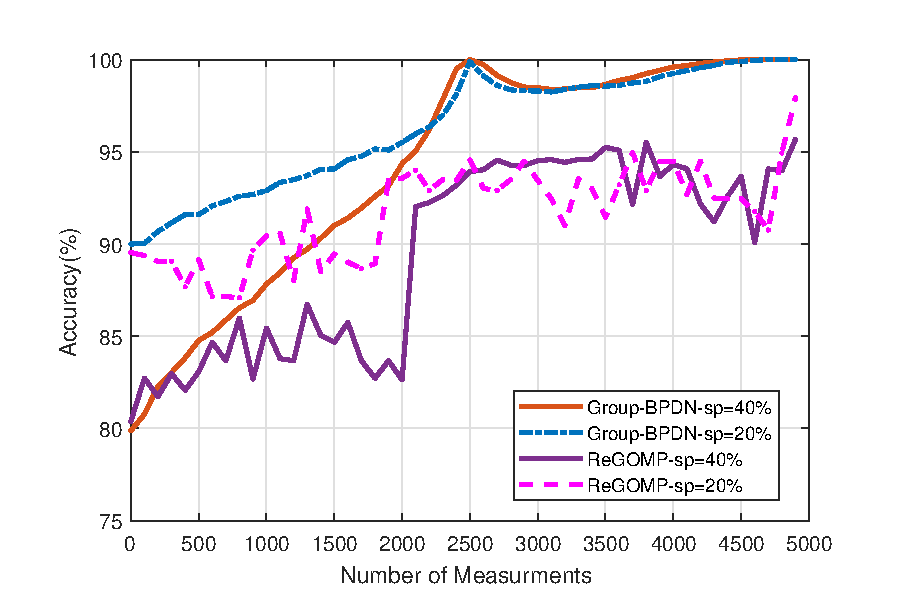
\includegraphics[width=0.95\textwidth]{figures/GC_beamforming/measuremDelay2sen4.eps}
	\caption{Comparison betweeen the proposed CS-CDMA scheme based on Group-BPDN and its modified version using ReGOMP. Maximum delay $= 2$ chip time duration, sparsity (sp) $= 20 \%$ and $= 40 \%$.}	
	\label{Fig_result3}
\end{figure}

\noindent \textbf{Network traffic and time:} With the proposed framework with  $L$=$64$, the total traffic flow in a transmission cycle becomes $32$ bytes, which is much lower than the existing IEEE 802.15.6 standard that requires a minimum of $13\times 4$ bytes as frame header alone not including the data. The time required for the whole transmission cycle
%with less transmission rate and tissue breathing time
is estimated using (\ref{time}) for $T_R$=$10\ \mu s$ and $\eta$=$100\ kbps$ to be only $1.3\ ms$ that is mainly dominated by the transmission time.



\noindent \textbf{With and without beamforming:} We next compare the energy consumption for the implant to relay communication through the M-S path with and without the beamforming. For an expected link length of $5\  cm$, the average M-S path-loss is $41.2\ dB$. The energy per bit required for a desired SNR of $\hat{\delta}$ is given using (\ref{eqn:Ptmin}) by $E_b$=$P_i^{min}/\eta$.   
For $\hat{\delta}$=$10$, a noise factor ($N_o$) of $1e$-$8$, data rate $\eta$ of $10 \ kbps$ and bandwidth $\triangle f$ being $1e5\  Hz$,  the required energy per bit ($E_b$) becomes $6.62\ \mu J$. This would allow battery of capacity of $240\ mAh$ to last for $2.89$ years. 
  
Before beamforming, the implants first broadcast their individual codewords in the M-M path. This step requires an energy of $0.68\ \mu J$, considering the same values as assumed above for all other parameters, other than the lower path loss through M-M path ($19\  dB$). The aggregated codeword is then transmitted from the aggregator as a broadcast to all implants that requires $\approx 0.7\mu J$. Finally, the beamforming towards the relay in undertaken in the M-S path, where each node spends about $4e$-$5M^{-1.03}$ times less energy than that actually required for the direct M-S path. For a scenario with 4 implants, the power consumption in each implants for the complete transmission cycle is $1.39\  \mu J$, which is $4.7$ times lower than that required for M-S communication without beamforming. The proposed framework extends the life of implant upto $13.8$ years assuming every other parameter remains the same.


\section{Conclusion}\label{sec:concl}
In this paper, we propose and implement an energy efficient implant to surface relay communication using galvanic coupling and beamforming. The proposed communication technique is strongly focused on improving energy efficiency by: sharing sensed updates among peer-implants using compressed sending CDMA through the high-gain M-M path, avoiding unpredictable data delivery conditions caused by collisions and transmission back-offs. Then, through near-field beamforming performed by the implants organized into distributed transmitter arrays, communication through the vertical tissue layers is achieved with high SNR (or conversely, lower energy per implant). The proposed framework dramatically lowers the net energy required for end-to-end implant to relay communication that is 79\% more energy efficient than the direct case, and extends the lifetime of implants upto $13$ years, while ensuring accurate, low BER communication.
\section*{Acknowledgement}
This material is based on the work supported by the U.S.
National Science Foundation under Grant No. CNS-1740907.





%%%%%%%%%%%%%%%%
% Chapter 7
%%%%%%%%%%%%%%%%

%\chapter{Galvanic coupling for intra-body communication links} 
\section{Introduction}
Implanted sensors will enable the next generation of healthcare by in-situ testing of abnormal physiological conditions, personalized medicine and proactive drug delivery. 
The paradigm of interconnecting the implants is known as intra-body network (IBN) 
and allows implants to transmit measurements to an external processing center for real time monitoring, to receive updates on drug delivery volumes, and to directly start actions by embedded actuators. 
All these examples require energy efficient data communication between implants through body tissues.

However, the state of the art (SoA) for intra-body communication (IBC) relies on high frequency radio (RF) signals. Short-range RF communication techniques, such as Bluetooth, ANT, and Zigbee \cite{Seyedi2013} are useless for intra-body communication as they are affected by severe attenuation  within the human tissues, which are composed of 40-60$\%$ water, high power consumption, and limited battery lifetime.
Moreover, emitted RF signals propagates also around the body, creating privacy risks.  

\subsubsection{Non-RF IBC techniques}
Non-RF techniques that use the human body as a medium for data communication include ultrasound (US) technology, which consists of mechanical vibrations and works well in mediums with high water content such as the body \cite{Galluccio2012}. The main US drawbacks are severe multi-path fading and the high delay caused by slow propagation speeds. Another alternative to RF is inductive coupling (IC) \cite{Park2015}: coils wrapped around anatomy are used to generate and receive magnetic energy and the efficiency of the data transfer is directly proportional to the coupling efficiency (i.e. correct resonance frequency matching between the transmitter and the receiver), which is not always easy to achieve. Capacitive coupling (CC) \cite{Seyedi2013} uses electrical signals with a couple of electrodes at the transmitter and receiver, respectively. Only one of the electrodes at each side is attached to the body while the other electrode is floating (ground electrode needs only to be in proximity) and the signal is generated between the body channel transceiver by making a current loop through the external ground. Thus, unfortunately, the path loss has high variability based on environmental conditions.

We use an alternative cable-less architecture for IBNs using galvanic coupling (GC) technology for communications among implants.
GC utilizes low or medium frequency (1 kHz-100MHz) and weak ($< 1mW$) electrical
currents, which are modulated with data and coupled directly to the tissue \cite{Callejon2014}.
Differently from SoA RF solutions, GC IBNs does not show privacy risks since the signals do not propagate outside the body, and consumes two orders of magnitude less energy than RF method \cite{Swaminathan2016,Swaminathan2017}.

\subsubsection{Related works}
Existing GC efforts focused on signal strength changes in tissues \cite{Seyedi2013, Wegmueller2009, Callejon2014} and the characterization of human tissues \cite{Swaminathan2016, Seyedi2013, Wegmueller2010}, which are a valuable base to explor the feasibility of communication schemes that are difficult to be performed directly on the human body.

Some works have been conducted in developing GC testbeds.
For example, a test system has been designed and implemented, 
%which includes four transmitting sensors and one receiver, sending data through a frequency division multiple access (FDMA) scheme, given the costant GC attenuation over the considered frequency range, and a differential binary phase-shift-keying (DBPK) modulation, with a throughput of $4.8$ kbps  \textcolor{red}{[WEGMULLER 2009]}. 
which considers a complex programmable logic device (CPLD) containing all the digital signal processing blocks of the transmitter, and, besides the analog units, a field-programmable gate array (FPGA) at the receiver to provide the digital demodulation and interfaces \cite{Wegmueller2009}.
More recently, a base band transmission has been implemented
in a FPGA board based on impulse radio (IR) employing a pulse position modulation (PPM) \cite{Seyedi2017}.
In \cite{Tomlinson2016} design a testbed using two USRP software defined radios (SDRs), one at the transmitter and the other at the receiver side, supporting  low frequency daughterboards.
%All the aforementioned test systems are valuable works but require specific equipments and softwares, so that their corresponding experiments are not quickly replicable.
Anyhow, an effective and repeatable GC platform to carry out experiments is still a challenge. 

\subsubsection{Proposed sound card based GC testbed}
We here design and implement a GC testbed that is based on PC sound card and Matlab environment, hence easily replicable for the interested research community. The main advantages of the proposed testbed architecture are that: (i) such scheme requires limited equipment since only ordinary PCs and Matlab software are needed; (ii) allows high flexibility since all parameters, including carrier frequency, bandwidth and modulation order, may be varied directly in the TX/RX Matlab programs allowing a quick evaluation of the resulting effects; (iii) real time option for the receiver by including a Data Acquisition Toolbox (Daq Tbx) in Matlab that exploits the real time data logging feature of the toolbox \cite{Hwang2013}, so that real time transmission and evaluation of physiological data sets are possible; (iv) BER evaluation of the experimental setup. 


\section{Background on GC communication technology}
\begin{figure}
	\includegraphics[width=\textwidth]{figures/GC_testbed/GC.png}
	\caption{GC setup on skin surface with detail on multiple tissues} \label{figGCtech}
\end{figure}

An alternative ultra-low power solution that uses the human body as a communication medium is GC technology. In GC, a pair of electrodes is used to directly couple a weak electric current into the human body, so that the electrical signal is applied differentially between the two electrodes of the transmitter and secondary paths of propagation are used for potential difference detection at the electrodes of the receiver \cite{Seyedi2013}.
Recommendetion from ICNIRP \cite{Banou2018} suggests to limit the signal within the safe bound of $1$ mA, which is easily matched from GC technology, usually injecting currents in the order of $0.5$ mA \cite{Tomlinson2018}.

Fig. \ref{figGCtech} represents the conceptual illustration of GC: the transmitter is composed of a pair of electrodes with typical distance of 5 cm (on-skin case is depicted in Fig. \ref{figGCtech}, although the electrodes could be places in any tissue) to inject low intensity electrical currents as data signals. While the primary current flows through the two transmitter electrodes, weak secondary electrical currents carry the information to a distant pair of receiver electrodes using layered tissues conduction. Experiments prove that a weak secondary current can be detected at the receiver with a transmission range of 20-30 cm. GC may use any type of electrode, whose usual size is approximately 10 mm \cite{Li2017}, and consumes only 0.24 nJ per received bit compared to 106 nJ/b of Zigbee \cite{Seyedi2013}. Indeed, due to its frequency range, the GC signal is restricted to the body so that GC communication is highly energy efficient, resulting in a long lifetime for battery-powered implants. The tissue heating is low due to the limited attenuation at the frequencies used, and communication is interference-free and secure from external fields.
The operative frequency range of GC is a tradeoff among tissue attenuation, interference with other natural signals (e.g., ECG and EEG signals), and other impairments. Experiments show that the usable frequency range is 1kHz-100MHz \cite{Callejon2014}, so that other natural signals are not impaired.

\subsection{Channel Model for the human body}
\label{GCChannel}
The main approaches modeling the electrical behavior of human tissues include
wave numerical techniques, for instance, finite element analysis (FEA) and finite difference time domain method (FDTD) \cite{Wegmueller2007,Song2012}, quasi-static approximations, \cite{Pun2011,Chen2012}, and equivalent circuit analysis (ECA) models.

Field analysis with FEA and FDTD are accurate but expensive for the required time computation.
The quasi-static approximations of field distribution are less computationally complex but only model low frequency Maxwell’s equations, so that they are not valid for high frequency applications.

The ECA model gives an easy transfer function with accurate gain calculation, and is valid for a wide range of frequency.
Several ECA methods focus on single tissue layer, such as \cite{Wegmueller2010}, while a recent analytical model has been proposed that considers a three dimensional multi-layered tissue, validated through finite element simulations \cite{Swaminathan2016}.

%\textcolor{red}{An empirical GC channel model based on stored channel impulse response and analysis of the channel frequency response, noise, and capacity reveal that the channel may be modelled as additive white gaussian noise (AWGN) \cite{Tomlinson2016,Tomlinson2015}}.

\subsection{Related works on GC testbed}
%\BOOK p. 22:
Some works have been conducted to develop GC testbeds with different hardware and software features, in order to validate the aforemnetioned channel models and/or prove the GC viability as IBC technology.

%\BOOK p. 23: 
A low power single chip biomedical system is designed in [40], firstly exploiting GC paradigm, with a continuous phase frequency shift keying (CPFSK) modulation scheme.

The test system in \cite{Wegmueller2007} includes battery powered transceiver and an FPGA as interface between analog front-end and digital communication link. Two modulation schemes have been used,  frequency shift keying (FSK) and binary phase shift keying (BPSK), with a 128 and 255 kbps, respectively.

In \cite{Cho2009}, the authors build up a transceiver to communicate with both on-body and implanted sensors with a frequency range in the order of tens to hundred MHz and a data rate up to 5 Mbps. 

Base band transmissions are developed in a FPGA board based on impulse radio (IR) with a PPM, and the corresponding BER performance is evaluated  \cite{Seyedi2017}.

A GC tesbed has been proposed recently based on off-the-shelf SDR platforms with low frequency daughterboards and Matlab environment, which presents BER performance for differential BPSK (DBPSK) modulation for different level of transmitted power in case of one transmitter and one receiver implant \cite{Tomlinson2016}, and BER QPSK performance in case of two transmitters and one receiver \cite{Banou2018}.

Finally, given the heterogeneity of experimental setups and conditions, and some discrepancies observed between results in literature, some studies have been conducted to evaluate the influence of different experimental settings on GC measurements \cite{Callejon2015}.
On that purpose, different experimental setups have been considered to analyze specific key issues such as load resistance, grounding, effect of cables, and type of measurement device \cite{Callejon2015}.

Anyhow, all the developed systems require specific hardware and software and show low flexibility, resulting in GC platforms difficult to replicate for carrying out experiments.

\section{GC testbed architecture}
\begin{figure}
	\includegraphics[width=13.5cm,height=6.5cm]{figures/GC_testbed/Fig_Architecture_tot_1.jpg}
	\caption{Experimental setup of the GC testbed} \label{figGCtestbed}
\end{figure}

Since the common sound cards support signals whose frequency range is included in the GC frequency range (1KHz-100MHz), we develop and implement a GC testbed for intra-body communication links employing only ordinary PCs with sound card support and Matlab software, resulting in a simple platform to emulate a single implanted sensor transmission/reception.

The developed system may be easily reproduced and is flexible since all the parameters may easily changend in the TX/RX Matlab programs, while allowing real time transmission of physiological data sets. 
%\textcolor{red}{The Matlab-based programs for the  transmitter and receiver are available at [REFERENCE] to allow a quick implementation of the testbed for the interested researchers, and stimulate further research in the field.}
The developed testbed manages all aspects of communication, including, among the others, bit generation, preamble insertion and raised cosine filtering.


\subsection{Blocks design of the GC system architecture}
The main advantage of the proposed GC system architecture is its limited equipment requirement, consisting of two common PCs with sound card and the basic Matlab package for transmitter and receiver development, as shown in Fig. \ref{figGCtestbed} and in the block diagram in Fig. \ref{figGCaudio}. Bridging the channel and the two PCs, we ensure to use battery powered PCs without connection to the grid, in order to isolate the common ground return paths of the transmitter and the receiver, as required from GC technology \cite{Banou2018}.

Fig. \ref{figGCaudio} illustrates that only two Matlab sessions are required, one per PC, to implement the transmitter and receiver respectively, and the sound cards are used to support real signal transmission/reception in a subset frequency range of GC technology \cite{Callejon2014}. On that purpose, Fig. \ref{figGCaudio} shows that the transmitted data generated through Matlab are converted from digital to analog domain to be sent over the sound card of the transmitter. A cable is connected to the \emph{LINE OUT} jack to carry the signal outside the PC. As detailed later, the cable is attached to two electrodes that represent the GC transmitter, which send the signal over the tissue through GC communication technology. At the other side, the two receiver's electrodes bring the received signal to the other PC through the cable connected to the \emph{LINE IN} jack. The data are thus processed in the Matlab session II where the receiver program is running. 

\begin{figure}
	\includegraphics[width=\textwidth]{figures/GC_testbed/AUDIO.jpg}
	\caption{Setup of the GC audio-band testbed using two PCs} \label{figGCaudio}
\end{figure}

In the following, the blocks diagram of the proposed audio-band GC system are described, including the functional blocks of the transmitter and the receiver,  shown in Fig. \ref{figTX} and \ref{figRX}, respectively. 
%while details about the channel are given in Sec. \ref{Impl} when describing the system implementation. 

\subsection{Functional blocks of the GC transmitter}

%\textcolor{red}{specifichiamo i nomi delle variabili nella fig. 4? ma non li abbiamo tutti}\\


%The transmitter implemented in Matlab includes bit generator, BPSK modulator, preamble insertion, oversampling, raised cosine filtering, up-conversion at the carrier frequency, digital to analog conversion to send the signal over the sound card and outside the PC through a cable connected to the two electrodes of the GC transmitter. 

Before detailing each block of the transmitter shown in Fig. \ref{figTX}, we summarize in the following Table \ref{tab1} the main parameters values of the system. Note that both transmitter and receiver parameters are included for completness.

\begin{figure}
	\includegraphics[width=\textwidth]{figures/GC_testbed/TX.png}
	\caption{Block diagram of the GC transmitter} \label{figTX}
\end{figure}

\begin{table}
	\caption{Parameters setting}\label{tab1}
	\begin{tabular}{|l|c|}
		\hline
		%\textcolor{red}{ft=1;} & $\%$ symbol frequency normalized \textcolor{red}{at packet time};\\ 
		$\mathbf{Parameter}$ & $\mathbf{Value}$\\  
		\hline
		Carrier frequency $f_c$ (KHz) & $15$\\ 
		Waveform sampling frequency $f_{s_a}$ (KHz) & $48$ \\ %waveform sampling frweq whose value matches the standard  sample frequency of PC sound card
		Oversampling frequency $f_s$ in number of samples & $4$\\ %normalized at sample time Ts
		Sampling time $T_s$ (ms) & $0.16$\\
		RX oversampling frequency $f_{s_{rx}}$ in number of samples & $2$\\ %normalized at sample time Ts
		roll-off of TRX filters $R$ & $0.2$\\ 
		delay of TRX filters  $D$ in number of samples & $8$\\
		%srrc=rcosine(ft,fs,'fir/sqrt',R,delay);& $\%$ coefficients of FIR root-raised-cosine filter;\\ 
		QAM modulation order$M$ & $2$\\
		RX Wiener filter length $N_f$ in number of samples & $11$\\ 
		%length of the RX Wiener filter normalized at symbol time (with oversampling $f_{s_{rx}}=2$)
		Modulated sequence $N$ in number of symbols & $1000$\\
		Preamble length $N_{pre}$ in number of symbols & $192$\\
		\hline
	\end{tabular}
\end{table}

Fig. \ref{figTX} shows that after bit generation, a preamble is inserted and the data are modulated in BPSK. The sequence is oversampled by 4, as specified in Table \ref{tab1}, and passes through a squared-root-raised-cosine (SRRC) filter. %as transmitter pulse shape, 
The corresponding baseband samples $x(nT_s)$ are thus generated, with  $n=0,1,...,f_sN-1$ and sampling time $T_s$.

The resulting sequence is then upconverted to the carrier frequency by multiplying it by the $cos$ signal, which represents the local oscillator (LO) obtained via software-define radio in Matlab program. This yields an audio passband transmitted signal  $s_{tx}$:

\begin{equation}
s_{tx}(nT_{s_a})= x(n T_{s_a}) \cos (2 \pi f_c n T_{s_a}) 
\end{equation} 

where %$x$ is the baseband signal after oversampling and filtering, $n=0,1,...,N$, 
$T_{s_a}=1/f_{s_a}$ with $f_{s_a}=48000$ Hz, whose value is chosen according to the standard sample frequency of PC sound card, and $f_c$ is the carrier frequency. According to the parameters setting in Table \ref{tab1}, $T_{s}=8$ $T_{s_a}$ with a net data rate $R=6$ kbs, in line with several biomedical applications showing sparse and low rate traffic generated by implanted sensors \cite{Swaminathan2017,Tomlinson2018}.
%under normal physiological conditions  
Anyhow, the achievable data rate may be incresed by appropriately choosing the value of $f_s$, $f_{s_a}$, $f_c$ shown in Table \ref{tab1}. 

Fig. \ref{figTX} illustrates that the obtained audible signal $s_{tx}$ passes through the sound card's internal amplifier, which may be replaced with an external amplifier circuit using Arduino. Then, the signal is sent out to the \emph{LINE OUT} jack by using the following simple Matlab statements in Table \ref{tab2}, which play the software-generated transmitted signal:

\begin{table}
	\caption{Matlab audio playing statements}\label{tab2}
	\begin{tabular}{|l l|}
		\hline
		sObj = audioplayer($s_{tx}$,48000);&   $\%$ To create an audioplayer object for signal Stx,\\ 
		& \phantom{xx}  using sample frequency at 48000 Hz\\  
		playblocking(sObj);	& $\%$ To play from beginning till playback completes\\
		\hline
	\end{tabular}
\end{table}

Through a wire, the output signal is then connected to two electrodes, that represent the GC transmitter.

\subsection{Functional blocks of the GC receiver}

\begin{figure}
	\includegraphics[width=\textwidth]{figures/GC_testbed/RX.png}
	\caption{Block diagram of the GC receiver} \label{figRX}
\end{figure}

The main blocks of the receiver developed in Matlab are shown in Fig. \ref{figRX} and may be split in the following two macro-blocks: (i) signal recording and digital down-conversion and (ii) burst detection and symbol timing estimation.

\subsubsection{Signal recording and digital down-conversion}
A Matlab session must to be open in the PC connected with the GC receiver for running the receiver program, which includes the following Matlab statements in Table \ref{tab3} to record the received signal and store the data in the array $s_{rx}$.


\begin{table}
	\caption{Matlab recording statements}\label{tab3}
	\begin{tabular}{|l l|}
		\hline
		recObj=audiorecorder(48000,16,1); &   $\%$ To create a 48000 Hz, 16-bit, 1 channel\\ & \phantom{xx} recorder object;\\
		Tsamp=1/48000;&  $\%$ Sampling time;\\
		Trecord=$N*f_s*T_{s_a}$;&  $\%$ Recording time, where: \\ & \phantom{xx} N is the modulated sequence lenght, \\ & \phantom{xx} fs is the oversampling freq equal to 16;\\
		recordblocking(recObj,Trecord+3);&   $\%$ To record for length of time, Trecord+3,\\ &  \phantom{xx} expressed in seconds;\\
		$s_{rx}$ = getaudiodata(recObj);&   $\%$ To return the recorded audio data\\ & \phantom{xx} as a double array.\\
		\hline
	\end{tabular}
\end{table}

As shown in Fig. \ref{figRX}, after recording the signal $s_{rx}$ in digital format, which passes through the sound card amplifier, a digital down-conversion is performed by multiplying the received sampled signal by $\cos (2 \pi f_{c} n T_{s_a})$, where $f_{c}$ is the carrier frequency at the receiver. The sequence then is sent to an SRRC filter, resulting in a baseband received signal $y(nT_{s_a})$ with $n=0,1,...,f_sN-1$. 
%\textcolor{red}{(va bene mettere Ts e Tsam uguale, e variare fc e theta e awgn come disturbi?)}

The output signal is then decimated by two so that the next blocks, described below, work at two samples per symbol ($f_{s_{rx}}=2$ as specified in Table \ref{tab1}). The obtained sampled signal may be expressed as

\begin{equation}
y(nT_s)=s_{tx}(nT_s) e^{j\theta}+v(nT_s)
\end{equation}

where $n=0,1,...,f_{s_{rx}}N-1$, $s_{tx}(nT_s)$ is the envelope samples of the passband signal, $v(nT_s)$ is the sampled AWGN noise, $\theta$ is the random phase noise due to time delay. 

\subsubsection{Burst detection and symbol timing estimation}

Being the packet composed by a preamble followed by data, the burst detection is performed by estimating the start of the preamble through a correlation method.
Specifically, the transmitted preamble, known at the receiver, is cross-correlated with the receveid data so that the position of the correlation's peak gives an estimated of the preamble start position:

\begin{equation}
\hat{t}_{p}= \argmax_n \left| \sum_{k=0}^{L-1}y((n+k)T_s)p^*(kT_s)\right| 
\label{eq_delay}
\end{equation}

where $\hat{t}_{p}$ is the estimate of the sample index where the reference preamble $p$ begins, $N_{pre}$ is the preamble's length, $L=f_{s_{rx}}N_{pre}$ 
since the receiver is working at two samples per symbol (oversampling frequency $f_{s_{rx}}=2$), and $n= 0, 1,...,f_{s_{rx}}N-1$.

%cross1=xcorr(x_tot,d_pre)
%t_r1=find(cross1==max(cross1))-length(x_tot);

Hence, the received signal is shifted in time according to the estimated start of the preamble $\hat{t}_{p}$ and is equalized with a Wiener filter, that also performs symbol timing improving the delay estimate obtained with (\ref{eq_delay}). 

The coefficients $w(i)$ of the filter, with $i=1,...,N_f$, are calculated by using the shifted received preamble $y_p(nT_s)=y(nT_s+\hat{t}_{p})$ and the known transmitted one $p(nT_s)$ with $n=0,1,...,f_{s_{rx}}N_{pre}-1$.
In more details, the vector $\mathbf{w}=\left[w_1,w_2,...,w_{N_f}\right]$ of the coefficients can be computed by minimizing the mean square error (MSE) between the transmitted and estimated preamble, defined as  
%\begin{equation}
%\label{eq_MSE}
%\epsilon=E\left\{\left[x(nT_s)-\hat{x}(nT_s)\right]^2\right\}
%\end{equation}
%%with  $n=0,1,...,f_{s_{rx}}N-1$. Npre invece di N perche' uso solo preambolo, ma già detto prima. 

\begin{equation}
\label{eq_MSE}
\epsilon=E\left\{\left[p(nT_s)-\hat{p}(nT_s)\right]^2\right\}
\end{equation}

Setting the following partial derivatives of the error (\ref{eq_MSE}) equal to zero
\begin{equation}
\label{eq_deriv}
\frac{\partial \epsilon}{\partial w_i}=0, \text{  for }i=1,2,...,N_f
\end{equation}

we can solve (\ref{eq_MSE}), (\ref{eq_deriv}) for the coefficients $w_i$ by inverting an autocorrelation matrix of size $N_f\times N_f$, which leads to the following Wiener-Hopf equation
%\begin{equation}
%\label{eq_Wiener}
%\mathbf{w}=\mathbf{R}_y^{-1}\mathbf{r}_{xy}
%\end{equation}
%where $\mathbf{R}_y=\{r_y(k)\}$ is the autocorrelation matrix whose elements are $r_y(k=j-l)=E\left\{y_j(i)y_l(i)\right\} $, and $\mathbf{r}_{xy}=\{r_{xy}(k)\}$ is the cross-correlation vector whose elements are defined as $r_{xy}(k)=E\left\{x(i)y_k(i)\right\}$, and $j,l=1,2,...,N_f$.

\begin{equation}
\label{eq_Wiener}
\mathbf{w}=\mathbf{R}_{y_p}^{-1}\mathbf{r}_{py_p}
\end{equation}
where $\mathbf{R}_{y_p}=\{r_{y_p}(k)\}$ is the autocorrelation matrix of the received preamble $y_p$, whose elements are $r_{y_p}(k)=E\left\{y_{p}(i-k)y_{p}(i)\right\} $, and $\mathbf{r}_{py_p}=\{r_{py_p}(k)\}$ is the cross-correlation vector between the transmitter preamble $p$ and the received one $y_p$, whose elements are defined as $r_{py_p}(k)=E\left\{p(i-k)y_{p_k}(i)\right\}$, and $i,k=1,2,...,f_{s_{rx}}N_f$.

After calculating the Wiener coefficients using only the preamble, the filter is applied to all the sequence, so that its output is the estimated transmitted sequence $\hat{x}(nT_s)$, expressed as
\begin{equation}
\label{eq_outW}
\hat{x}(nT_s)=\sum_{l=0}^{N_f-1}w(lT_s)y((n-l)T_s+\hat{t}_{p})
\end{equation}

%Note that, since we are employing the Wiener filter in place of a matched Nyquist filter, we have $N_f=2q+1$ where $q$ is the number of the finite impulse response (FIR) Wiener coefficients, so that $\mathbf{w}$ may be expressed as $\left[w_{-q},...,w_{0},...,w_{q}\right]$ and $r_{xy}(k)=\sum_{l=-q}^{q}w(l)r_y(k-l)$, with $k=-q,...,q$.










%\textcolor{red}{filtro Wiener (sostitusce srrc) è adattativo (invece srrc è adattato) e fa insieme 3 cose: equalizza (se i coeff dei filtri fanno qualcosa in freq), recupero fase, e timing di clock (diverso da timimg di pacchetto che stimiamo con synchro con max correlaz); uso inviato filtrato due volte (dd) e ricevuto con awgn che viene filtrato due volte (sn2)}

After a downsampling operation at one sample per symbol, the BPSK symbol sequence is demapped to a bit sequence and the preamble is removed, thus completing the receiver operations. The obtained bit sequence may be hence compared to the transmitted one for BER calculation.
 
\subsection{Implementation of the GC system}
\label{Impl}
%\textcolor{red}{AWGN se senza filo ma solo programmi con dati inviati salvati?}
Before evaluating the performance of the overall system with a real tissue-based GC channel, we first test only the transmitter and the receiver, for which the configuration in Fig. \ref{FigWIRE} is considered. Then, 
%a simulated channel is included in such setting, and finally 
an experimental setup is evaluated with real tissue for GC transmissions as in Fig. \ref{figGCaudio}. 

Fig. \ref{FigWIRE} derives from Fig. \ref{figGCaudio} by substituting the steak with a simple wire connecting the \emph{LINE OUT} sound card's jack of the PC running the Matlab transmitter program with the \emph{LINE IN} jack of the other PC running the receiver program.
\begin{figure}
	\includegraphics[width=\textwidth]{figures/GC_testbed/AUDIO_WIRE.jpg}
	\caption{Audio-band testbed using two PCs and a wire} \label{FigWIRE}
\end{figure}

%\subsubsection{GC system with simulated channel}
%\textcolor{red}{As specified in Sec. \ref{GCChannel}, the behavior of the GC channel may be simulated through an additive white gaussian noise (AWGN) channel \cite{Tomlinson2016,Tomlinson2015}.} 
%The proposed sound-card based testbed will be used also to validate such empirical results.
%Specifically, considering the setting in Fig. \ref{FigWIRE}, the channel is modeled with a delay on the received signal and an AWGN, whose Matlab commands are included in the receiver program after the recording statements. 
For the final setting, shown in
Fig.  \ref{figGCtestbed} and \ref{figGCaudio},
%We simulate the GC channel in the setting of Fig. \ref{FigWIRE} by introducing a delay on the received signal and applying an AWGN. The corresponding Matlab commands are included in the receiver program after the recording statements specified in Table \ref{tab3}. Sec. \ref{Exp} shows the performance of the proposed architecture in such setting as first evaluation test.
%\subsubsection{GC system with experimental channel}
%The proposed architecture 
the wire connecting \emph{LINE IN} and \emph{LINE OUT} jacks of the two PCs is cutted and each of its two parts are attached to the electrodes of the GC transmitter and receiver, respectively. Since the wire is composed by three electric clables, two of them are connected to the electrods on each side, while the third one remains floating. Under this configuration, the two transmitter and receiver Matlab session runs in parallel to perform the experimental evaluation detailed in the following section.




\section{Experimental Setup and Performance Evaluation}
\label{Exp}
%\textcolor{red}{Ptx max 12 mW per cui se metto volume al 70$\%$ ho 8.4 mW}

After testing the architecture in the configuration shown in Fig. \ref{FigWIRE}, which have confirmed the feasibility of the proposed transmitter and receiver architecture, we have conducted experiments in the final real scenario shown in Fig. \ref{figGCtestbed} and Fig. \ref{figGCaudio}. 
The parameters setting is detailed in Table \ref{tab1}, and the average BER is calculated over $100$ iterations. 

Note that we use really small size electrodes (in the order of $0.5$ mm) while the SoA is employing $1$ cm electrodes \cite{Li2017}. Although such choice would reduce the achievable distance between GC transmitter and receiver, in this way we test a real configuration scenario for future miniaturized implantable devices. 
The inter-distance between the electrodes at both the transmitter and receiver is set equal to $1$ cm, while the distance between the transmitter and receiver is varied during the experiments, together with the transmit power.

\begin{figure}
	\includegraphics[width=\textwidth]{figures/GC_testbed/TX_freq.eps}
	\caption{Transmitted signal in frequency domain} \label{FigTXfreq}
\end{figure}

\begin{figure}
	\includegraphics[width=\textwidth]{figures/GC_testbed/RX_freq}
	\caption{Received signal after RX filter in frequency domain} \label{FigRXfreq}
\end{figure}

Fig. \ref{FigTXfreq} and Fig. \ref{FigRXfreq} show the transmitted and received signal in the frequency domain, respectively, for $3$ cm distance between GC transmitter and receiver. Fig. \ref{FigTXfreq} refers to the transmitted signal before being modulated on the carrier frequency, as well as Fig. \ref{FigRXfreq} illustrates the received signal after demodulation and filtering. The comparison between the two figures confirms that the received signal exibiths the same shape of the transmitted one, since the side lobe of the receiver signal is maintained low by the filter being its amplitude around $90$ dB less than the main one. 
%The difference in the phase between the two transmitted and received signals is due to the time delay, which is correctly detected and compensated only in the block after the RX filter, while Fig. \ref{FigRXfreq} shows the signal before such compensation (see the receiver blocks in Fig. \ref{figRX}).     

\begin{figure}
	\includegraphics[width=0.85\textwidth]{figures/GC_testbed/BER_TXpower}
	\caption{BER vs transmit power for different distances between GC transmitter and receiver} \label{FigBER}
\end{figure}

Fig. \ref{FigBER} shows BER performance by varying the transmit power for different distance values between transmitter and receiver. As expected, BER performance decreases when increasing the distance, although the performance for $2$, $4$, $6$ cm result to be quite similar. We are able to achieve a BER in the order of $10^{-4}$ with $9.5$ dBm transmit power for $1$ cm distance, reaching $7 \cdot 10^{-3}$ for $10$ cm, a valuable result considering the small electrode size of $0.5$ mm and the simple receiver that is not employing any correction code. More robust receiver may be envioned based on ultra wideband (UWB) to improve the performance while mantaining simple and energy efficient receiver \cite{Alesii2015}, as required by biomedical implantable devices.    


\section{Conclusions}

We have proposed a sound card based GC testbed as a quick repeatable platform to carry out experiments. The detailed description of the implemented test system may support the interested researchers in replicating the testbed and thus stimulate further research in the GC field.
Experimental tests on real chicken tissue as GC communication channel have been conducted to prove the feasibility of the proposed architecture.
We achieve a BER in the order of $10^{-3}$ with  $9.5$ dBm transmit power for distances in the range $2-10$ cm, employing an simple receiver and electrodes with really small size ($0.5$ cm), while the SoA is usually employing $1$ cm electrodes.
Ongoing works include exstensive simulation to evaulate the effect of the carrier frequency, bandwidth, audio sampling frequency, electrodes size, as well as inter-electrodes distance at both the transmitter and receiver. Moreover, we are implementing an extension of the proposed testbed with Arduino platform in order to modulate the signals on a frequency range larger than the audio signals. Future research directions will exploit compressed sensing (CS) and UWB techniques to save time and energy \cite{Banou2018,Alesii2015}, a strict requirements in intra-body networks for medical applications.

% Chapter 8
%%%%%%%%%%%%%%%%

%\chapter{Phase recovery of XPIC receivers
}

Reduced complexity Kalman based algorithms are proposed to recover the phase of cross-polar interference cancellation (XPIC) receivers in microwave radio relay links. In particular, two completely independent radio frequency (RF) transceiver chains are considered for the two different polarizations, in order to have the maximum flexibility to connect different single carrier transceivers to dual-polarized antennas.
A one-state Kalman model is proposed, which is of low complexity and thus suitable for a modern higher data rates M-ary quadrature amplitude modulation (M-QAM) receiver. Moreover, a further reduced complexity version is developed that uses a lower amount of information to recover the phase at the receiver, as well as a downsampling procedure to speed up the Kalman algorithm, and an alternative error computation that is essential to ease the Kalman implementation. It is worth noting that the three last simplifications are general and can be applied not only to a one-state Kalman model.
Simulation results compare the proposed simplified Kalman solutions to typical phase-locked loop (PLL) algorithms proving their comparable performance with the benefit of lower complexity. Finally, the relationships between the Extended Kalman and the PLL approaches are investigated. The obtained relation is essential for the cross-polar phase recovery, since, as far as the authors know, there are not closed form solutions for the PLL parameter optimization in cross schemes.


%\begin{keyword}
%Kalman filter\sep phase recovery\sep cross-polar interference cancellation (XPIC)\sep digital receiver\sep  backhaul
%\end{keyword}

%\end{frontmatter}

%\linenumbers

\section{Introduction}

The recent spread of smart applications has led to the growth of data traffic in the last years.
As a result, the development of fifth-generation (5G) communications technology is required to fulfill the increasing users' traffic requirement. 
On this purpose, operators and carriers are claimed to improve the user experience and, in general, the overall network performance. 
In this sense, there are notable market interests on the development of innovative backhaul solutions to accommodate the increased wireless traffic and the resulting higher bandwidth demand \cite{Xiaohu}.

Cross polarization interference cancellation (XPIC) technology represents the enabler for dual-polarized transmissions over the same radio frequency (RF) channel, so that the \textcolor{black}{link capacity} is doubled by using two orthogonal polarizations channels over the same link \cite{Noel}. 

In order to have the maximum flexibility from an installation and maintenance point of view, some XPIC architectures are based on two independent and unsynchronized transceiver paths for backhaul links, with completely independent transmitter and receiver local oscillators (LOs) \cite{Rossi}.

Differently from multiple input multiple output (MIMO) solutions that work with a carrier-over-interference ratio ($C/I$) almost equal to $0$ dB, XPIC operating conditions have cross polarization discrimination (XPD) around $20-25$ dB. \textcolor{black}{Despite the fact that} such XPD value could be considered almost error free for low order modulations, higher order QAM schemes still could represent a challenge \cite{Noel2}\cite{Proenca}, for example they highly suffer from phase noise even in line of sight (LoS) environments.

Carrier frequency and phase synchronization are also challenging for higher order M-QAM single polarization receivers, and may be accomplished by a Kalman algorithm, as described in \cite{Campeanu}\cite{Wei-Tsen}.

In \cite{CommLett}, we proposed a cross-polarized Kalman based phase recovery scheme for an XPIC architecture that jointly recovers the phase of both the received signal and the interfering one at the input of the cross-polar interference canceller. \textcolor{black}{In particular}, a four-state extended Kalman filter (EKF) algorithm for an XPIC receiver was derived, along with a modified version that exploits two simpler two-state EKFs, one for the main polarization path and the other for tracking the interference signal phase.


In this paper, starting from the two-state Kalman model for a XPIC receiver \cite{CommLett}, we focus on studying the computational complexity of such schemes in order to develop practical architectures that could be \textcolor{black}{efficiently implemented} in modern digital hardware for high data rate microwave backhaul links. We think that computational aspects are crucial to make the Kalman based architecture more attractive with respect to the simpler \textcolor{black}{one based on} two phase-locked loops (PLLs), especially from a hardware feasibility point fo view. \textcolor{black}{Moreover, we think that a comprehensive study of the performance-complexity trade off is crucial in order to help the interested technical community in developing real hardware prototypes of the scheme proposed in \cite{CommLett}.}



\textcolor{black}{The main contributions of the paper are listed in the following:}
\begin{itemize}
	
	\item \textcolor{black}{a low complexity Kalman filter scheme is proposed for phase recovery in XPIC systems, based on two one-state EKFs. Although such solution shows a lower computational burden with respect to the scheme in \cite{CommLett}, it provides similar or anyway acceptable performance.}
	\item \textcolor{black}{the performance of the presented scheme is also evaluated by studying the effects of the following complexity reduction algorithm implementations:}
	\begin{itemize} 
	\item \textcolor{black}{The computational burden needed for computing the covariance matrix inverse may be reduced.} Specifically, since the phase noise variations are slow respect to the symbol timing, the covariance matrix computation update may be kept constant during several Kalman iterations without affecting the overall algorithm performance. This is equivalent to make a downsampling only inside the covariance matrix computation loop; 
		\item the phase-error computation is modified in order to avoid two phase counter-rotations in the Kalman state update equations. In this way the hardware design is more feasible, since phase rotation are computationally expensive;
		\item complexity reduction \textcolor{black}{is also achieved} by considering in the phase error computation only the in-phase or in-quadrature component of the signals.
	\end{itemize}

	 	\item \textcolor{black}{the relation between the Extended Kalman Filter (EKF) based approach and the commonly used PLL parameters is extensively studied}. While \cite{Patapoutian} probes the relation between Kalman and PLL gains, we investigate the connection between the Extended Kalman version and the PLL. This relation is important for the cross-polar phase recovery, since, as far as the authors know, while there are closed form solutions for PLL parameters in single polarization receivers, they do not exist for the cross PLL parameter optimization. Indeed, such EKF-PLL relation could be useful to optimize cross PLL parameters through EKF simulations. In particular, being the PLL implementation easier than a Kalman scheme, we envisage a final practical solution where a typical cross PLL scheme with fixed gains is replaced by a cross PLL with variable gains, which are calculated through Kalman simulation, resulting in a solution more robust to channel variations.
\end{itemize}

The paper is organized as follows: Sec. \ref{SM} describes the system model, Sec. \ref{Kalm2state} briefly reviews the EKF models described in \cite{CommLett}, while Sec. \ref{KalmReduced} analyzes the proposed reduced complexity Kalman schemes and the relation between the EKF parameters and the PLL filter gains. 
Sec. \ref{Results} shows some interesting simulation results, and, finally, concluding remarks wrap up and close the paper in Sec. \ref{Concl}.

\section{System Model}
\label{SM}

\begin{figure}
	\centering
	\includegraphics[width=1\textwidth]{figures/fig_red_kalman/Fig1.pdf}
	\caption{System Architecture}
	\label{Fig1}
\end{figure}


We consider a backhaul link with two distinct receiver paths and unsynchronized local oscillators (LO), as in \cite{Rossi}, \cite{CommLett}. Fig. \ref{Fig1} depicts the considered XPIC architecture, highlighting the two distinct receiver paths, with unsynchronized local oscillators (LO) for a backhaul link \cite{Rossi}. Since our focus is a typical microwave backhaul application, we model the channel with only AWGN without multipath fading as in \cite{CommLett}.

Let us consider the signal $r_0(n)$, received at one polarization path:

\begin{equation}
r_0(n)=t_0(n)e^{j\theta(n)}+gt_1(n)e^{j\phi(n)}+w(n)
\label{eq_r0}
\end{equation}

where $t_0(n)$ is the $n^{th}$ complex QAM transmitted symbol of the main polarization component with phase $\theta(n)$, $g$ is the cross-polar attenuation factor, $t_1(n)$ is the $n^{th}$ complex QAM symbol transmitted on the interference path with phase $\phi(n)$, and $w(n)$ represents the additive white Gaussian noise (AWGN) at the receiver.

The \textcolor{black}{aim} of both the Kalman and PLL algorithms is to estimate the phases ${\theta}(n)$ and  ${\phi}(n)$, along with the corresponding frequencies ${\dot{\theta}}(n)$ and ${\dot{\phi}}(n)$, by using the input of the main polarization slicer:
\begin{equation}
u_0(n)=\left(r_0(n)-gt_1(n)e^{-j\hat{\phi}(n)}\right)e^{-j\hat{\theta}(n)}
\label{outsig}
\end{equation}
where $\hat{\phi}(n)$ and $\hat{\theta}(n)$ represent the estimated phases of the main and cross polar signals at the receiver.
The cross-polar attenuation factor $\mathit{g}$ is assumed to be known, since, in high-order M-QAM receivers for microwave backhaul links, a linear filter interference canceller/equalizer is able to converge in presence of both baseband phase and frequency errors, providing a good initial guess for the PLL or the Kalman algorithms. Usually, during the acquisition phase, the adaptive linear filter works in a blind mode, typically by a constant modulus algorithm (CMA), and switches to a minimum mean square error (MMSE) algorithm once the normal operating condition is reached. Once the equalizer switches to MMSE, all the others recovery algorithms, like the Kalman phase recovery one, start using the decisions at the output of the slicer. 
In the following Sec. \ref{Kalm2state}, we give a short outline of the phase recovery using the two-state Kalman models \cite{CommLett}, and then, in Sec. \ref{KalmReduced}, we describe the proposed solutions, which include (i) a one-state Kalman model, (ii) a further simplified one-state version that uses a lower amount of information to recover the phase, and (iii) a downsampling of the covariance matrix computations to speed up the Kalman algorithm. All the proposed schemes aims to reduce the complexity of a Kalman based solution in a smart way in order to not degrade the performance. An alternative error computation \textcolor{black}{that can decrease the computational load of} Kalman implementation is also included, as well as some interesting relations between the Kalman and PLL parameters, useful for cross PLL parameters optimization, which is still missing.

\section{XPIC Phase Recovery Based on Kalman Filtering}

Since our purpose is to estimate the phase and the frequency of the signals in an XPIC scheme, such variables are considered in the Kalman state vectors.
We also define the observation vectors and the error to be minimized through the Kalman approach in order to obtain the estimates of the signal frequency and phase discrete values.\\	
Specifically, we consider a two-state XPIC Kalman algorithm for the main path and another one for the cross polar interference, so that the two-state vectors of the main and cross polar signals are expressed \cite{CommLett}:


%\setcounter{equation}{23}
\begin{equation}
\mathbf{x}_0(n)=\left[\begin{array}{c}
\theta(n)\\
\dot{\theta}(n)\\
\end{array}\right]
\label{eq_xx}
\end{equation}

\begin{equation}
\mathbf{x}_1(n)=\left[\begin{array}{c}
\phi(n)\\
\dot{\phi}(n)\\
\end{array}\right]
\label{eq_xx2}
\end{equation}

The state evolution of the linearized Kalman filter results:

%\setcounter{equation}{23}
\begin{equation}
\mathbf{x}_0(n)=\left[\begin{array}{c}
\theta(n)\\
\dot{\theta}(n)\\
\end{array}\right]=\mathbf{F}\left[\begin{array}{c}
\theta(n-1)\\
\dot{\theta}(n-1)\\
\end{array}\right]
\label{eq_xh}
\end{equation}

and

%\setcounter{equation}{24}
\begin{equation}
\mathbf{x}_1(n)=\left[\begin{array}{c}
\phi(n)\\
\dot{\phi}(n)\\
\end{array}\right]=\mathbf{F}\left[\begin{array}{c}
\phi(n-1)\\
\dot{\phi}(n-1)\\
\end{array}\right]
\label{eq_xv}
\end{equation}

where the transition matrix $\mathbf{F}$ is defined as

\begin{equation}
\mathbf{F}=\left[\begin{matrix}
1 & 1  \\
0 & 1  \\
\end{matrix}\right]
\label{eq_F2}
\end{equation}
The transition matrix definition $\mathbf{F}$ takes into account the fact that the residual carrier frequency offset at the PLL/Kalman input is usually lower than the initial one at the modem input, since a first stage coarse frequency detector is able to make it smaller. Moreover, the frequency offset time variations are anyway slower compared to the phase noise random fluctuations. 

While the cross polar observation vectors for the main and cross polarization signal, $\mathbf{r}_0(n)$ and $\mathbf{r}_1(n)$ respectively, are defined as

\begin{equation}
\begin{array}{ll}	
\mathbf{r}_0(n)=\mathbf{h}_0(\mathbf{x}_0(n))+\mathbf{w}_0(n)\\
\\
\mathbf{r}_1(n)=\mathbf{h}_1(\mathbf{x}_1(n))+\mathbf{w}_1(n)\\
\label{eq_r1}
\end{array}
\end{equation}
where
	\begin{equation}
	\mathbf{r}_0(n)=\left[\begin{array}{c}
	Re(\tilde{r}_0(n))\\
	Im(\tilde{r}_0(n))\\
	\end{array}\right],\;
	\mathbf{r}_1(n)=\left[\begin{array}{c}
	Re(g t_1(n))\\
	Im(g t_1(n))\\
	\end{array}\right]
	\label{eq_r}
	\end{equation}
	and $\mathbf{h}_0(\mathbf{x}_0(n))\doteq \mathbf{h}_0(n)$ and $\mathbf{h}_1(\mathbf{x}_1(n))\doteq \mathbf{h}_1(n)$ are the observer vectors, defined as
\begin{equation}
\mathbf{h}_0(n)=\left[\begin{array}{c}
\phantom{i}Re(\hat{t}_0(n)e^{j\theta(n)})\phantom{i}\\
\phantom{i}Im(\hat{t}_0(n)e^{j\theta(n)})\phantom{i}\\
\end{array}\right],\;
\mathbf{h}_1(n)=\left[\begin{array}{c}
Re(g\hat{t}_1(n)e^{j\phi(n)})\\
Im(g\hat{t}_1(n)e^{j\phi(n)})\\
\end{array}\right]
\label{eq_r}
\end{equation}
$\hat{t}_0(n)=\hat{a}(n)+j\hat{b}(n)$ is the output of the symbol \textcolor{black}{slicer}, $\tilde{r}_0(n)=r_0(n)-g\hat{t}_1(n)e^{-j\phi(n)}$, and:
\begin{equation}
\label{eq8}
g\hat{t}_1(n)e^{j\phi(n)}=r_0(n)-\hat{t}_0(n)e^{j\theta(n)}=\hat{c}(n)+j\hat{d}(n)
\end{equation}
While $\mathbf{w}_0(n)$ and $\mathbf{w}_1(n)$ are the observation noise on the main and interference path, respectively.
The EKF algorithms minimize the two distinct correspondent error vectors $\mathbf{e}_0(n)$ and $\mathbf{e}_1(n)$ defined as
\begin{equation}
\begin{array}{ll}	
\mathbf{e}_0(n)=\mathbf{r}_0(n)- \mathbf{h}_0(n)\\
\\
\mathbf{e}_1(n)=\mathbf{r}_1(n)- \mathbf{h}_1(n)\\
\label{eq_r2}
\end{array}
\end{equation}

The complete derivation of the EKF iterative equations may be found in section III of \cite{CommLett}.

\section{Proposed Reduced Complexity Kalman Algorithms}
\label{KalmReduced}

\subsection{One-State Kalman Model}
In this section, a simplified one-state Kalman model is developed for an XPIC scheme where only the phase of the signal is considered as state parameter, while the frequency is processed as an external input, obtaining a substantial complexity reduction. The proposed one-state model is derived starting from the two-state Kalman model \cite{CommLett}, in a way similar to the single-polarization scheme in \cite{Wei-Tsen}.

The one-state model can be represented as
%\setcounter{equation}{33}
\begin{equation}
\begin{array}{c}
x_0(n)=\theta(n)+\dot{\theta}(n)+v_0(n)\\
\\
x_1(n)=\phi(n)+\dot{\phi}(n)+v_1(n)\\
\end{array}
\label{eq_x1s}
\end{equation}
\textcolor{black}{where $v_0(n),v_1(n)$ represent the state noise signals.}
In the following we use the outputs of the hard decision 
$\hat{t}_0(n)=\hat{a}(n)+j\hat{b}(n)$ and $g\hat{t}_1(n)=\hat{c}(n)+j\hat{d}(n)$ 
to estimate the frequency $\dot{\theta}(n)$ and $\dot{\phi}(n)$. Note that the symbol $\hat{c}(n)+j\hat{d}(n)$ is always obtained from the slicer decisions of the main polarization component signal as follows:
\begin{equation}
\hat{c}(n)+j\hat{d}(n)=r_0(n)-\hat{t}_0(n)e^{j\hat{\theta}(n)}
\label{eq_gt12}
\end{equation}
which implies that the main path does not requires any feedback from the cross polar component, so that the two links work independently in a reciprocal blind manner.

The frequencies are computed by means of two first order loops:
\begin{equation}
\begin{array}{c}
\hat{\dot{\theta}}(n)=\hat{\dot{\theta}}(n-1)+K_{\theta i}Im\left\lbrace \textcolor{black}{u_0(n)}(\hat{a}(n)+j\hat{b}(n))^*\right\rbrace \\
\\
\hat{\dot{\phi}}(n)=\hat{\dot{\phi}}(n-1)+K_{\phi i}Im\left\lbrace \textcolor{black}{u_1(n)}(\hat{c}(n)+j\hat{d}(n))^*\right\rbrace \\
\label{eq_freq1s}
\end{array}
\end{equation}
where 
\begin{equation}
u_0(n)=(r_0(n)-gt_1(n)e^{-j\hat{\phi}(n)})e^{-j\hat{\theta}(n)}=\tilde{r}_0(n)e^{-j\hat{\theta}(n)}
\end{equation}
represents the phase corrected estimation of the main polarization received symbol, and $u_1(n)=-gt_1(n)e^{-j\hat{\phi}(n)}$ is the phase corrected estimation of the cross polar interference signal, according to (\ref{outsig}). $K_{\theta i}$, $K_{\phi i}$ are the integral gains which control the convergence rate of the frequency estimation algorithm and correspond to the integral loop parameter of a second-order PLL. $Im\left\lbrace . \right\rbrace $ is the imaginary part of its argument, while the symbol $^*$ represents the complex conjugate.

Equation (\ref{eq_freq1s}) is equivalent to a first-order PLL, so it has a lower performance compared to the complete two-state Kalman model described in Sec. \ref{Kalm2state}. Anyway, the complexity reduction makes its implementation \textcolor{black}{simpler} than a two-state Kalman scheme and comparable with a more common second-order PLL solution. 

The state equations for the one-state Kalman filter approach are given as follows in (\ref{eq_ph1s}), (\ref{eq_ph21s}):
%\setcounter{equation}{36}
\begin{equation}
\begin{array}{c}
\hat{\theta}(n|n)=\hat{\theta}(n|n-1)+\mathbf{K}_{\theta}\left(\mathbf{r}_0(n)-\mathbf{h}_0(n)\right)\\
\\
\hat{\phi}(n|n)=\hat{\phi}(n|n-1)+\mathbf{K}_{\phi}\left(\mathbf{r}_1(n)-\mathbf{h}_1(n)\right)\\
\label{eq_ph1s}
\end{array}
\end{equation}
%\setcounter{equation}{36}
\begin{equation}
\begin{array}{c}
\hat{\theta}(n+1|n)=\hat{\theta}(n|n)+\hat{\dot{\theta}}(n)\\
\\
\hat{\phi}(n+1|n)=\hat{\phi}(n|n)+\hat{\dot{\phi}}(n)\\
\label{eq_ph21s}
\end{array}
\end{equation}
where $\mathbf{K}_{\theta}(n)$, $\mathbf{K}_{\phi}(n)$ are the Kalman gains, while the errors are defined according to \textcolor{black}{the }equations (\ref{eq_r2}).

The one-state EKF may be derived according to
\begin{equation}
\begin{array}{c}
\mathbf{H}_0(n)=\dfrac{\delta \mathbf{h}_0}{\delta x_0}\arrowvert_{x_0=\hat{\theta}(n|n-1)}=\\
\\
=\left[ \begin{matrix} -\hat{a}(n)\sin(\hat{\theta}(n|n-1))-\hat{b}(n)\cos(\hat{\theta}(n|n-1))\\-\hat{b}(n)\sin(\hat{\theta}(n|n-1))+\hat{a}(n)\cos(\hat{\theta}(n|n-1))\end{matrix}\right]
\end{array}
\label{eq_H0s}
\end{equation}
\begin{equation}
\begin{array}{c}
\mathbf{H}_1(n)=\dfrac{\delta \mathbf{h}_1}{\delta x_1}\arrowvert_{x_1=\hat{\phi}(n|n-1)}=\\
\\
=\left[ \begin{matrix} -\hat{c}(n)\sin(\hat{\phi}(n|n-1))-\hat{d}(n)\cos(\hat{\phi}(n|n-1))\\-\hat{d}(n)\sin(\hat{\phi}(n|n-1))+\hat{c}(n)\cos(\hat{\phi}(n|n-1))\end{matrix}\right]
\end{array}
\label{eq_H1s}
\end{equation}

\subsubsection{One-State Model with Reduced Observations}
Following the same approach in \cite{Wei-Tsen}, it is possible to further reduce the implementation complexity by only considering the in-phase or the in-quadrature component in the two-dimensional equations (\ref{eq_r2},\ref{eq_ph1s},\ref{eq_H0s},\ref{eq_H1s}). 

\subsection{Alternative Error Detection Computation}
\label{Kalm2err}
In the following we formulate a new way of computing the minimized error in (\ref{eq_ph1s}), as an alternative to the model proposed in \cite{CommLett}, which provides the following main advantages:
\begin{itemize}
	\item it saves a phase counter-rotation in (\ref{eq_ph1s}) as shown in (\ref{err01}), which is usually hardware expensive;
	\item the one-state Kalman error is the same residual phase error used to drive the frequency estimations in (\ref{eq_freq1s}) which can be computed once for both the algorithms at each symbol time, thus saving computational operations.
\end{itemize}

The Kalman errors in (\ref{eq_ph1s}) corresponds to
\begin{equation}
\begin{array}{c}
e_0(n)=\tilde{r}_0(n)-\hat{t}_0(n)e^{j\hat{\theta}(n)}\\
e_1(n)=gt_1(n)-g\hat{t}_1(n)e^{j\hat{\phi}(n)}
\end{array}
\label{err01}
\end{equation}

In the following, we consider only the new error computation $\epsilon_0(n)$ corresponding to the main polarization error $e_0(n)$, since the same procedure can be replicated for $e_1(n)$.

The new computed error $\epsilon_0(n)$ is equal to the difference between the phases of the input and output of the symbol slicer as expressed in (\ref{eq_eps2_b}).

\begin{equation}
	\epsilon_0(n)=t_0(n)e^{-j\hat{\theta}(n)}(e^{j\theta(n)}-e^{j\hat{\theta}(n)})
	\label{eq_eps2_b}
\end{equation}

If we only consider the phase noise  contribution at the output of the interference canceler, the input of the main polarization slicer $u_0(n)$ in (2) can be recomputed as follows

\begin{equation}
u_0(n)=\tilde{r}_0(n)e^{-j\hat{\theta}(n)}=t_0(n)e^{j(\theta(n)-\hat{\theta}(n))}
\label{eq_s0_b}
\end{equation}
%
%Then, we calculate the new error detection $\epsilon(n)$ as
%
%\begin{equation}
%\epsilon(n)=\tilde{r}_0(n)e^{-j\hat{\theta}(n)}-\hat{t}_0(n)
%\label{eq_eps_b}
%\end{equation}
%
%which, under the hypothesis $\hat{t}_0(n)=t_0(n)$ becomes

Defining $s_0(n)$ as in the following

\begin{equation}
\begin{array}{lll}
s_0(n)=\epsilon_0^*(n)u_0(n)=\\
\\
\phantom{xxii}=|t_0(n)|^2e^{-j\hat{\theta}(n)}(e^{-j\theta(n)}-e^{-j\hat{\theta}(n)})e^{j(\theta(n)-\hat{\theta}(n))}=\\
\\
\phantom{xxii}=|t_0(n)|^2\left(-2j\sin\left(\frac{\Delta\theta}{2}\right)\right)e^{\frac{\Delta\theta(n)}{2}} 
\end{array}
\label{eq_u_b}
\end{equation}

where $\Delta\theta(n)=\theta(n)-\hat{\theta}(n)$ represents the difference between the true phase and the estimated one, i.e. the phase error at the output of the slicer. $\Delta\theta(n)$ may be computed, as usual in digital PLL, as in (\ref{eq_ph1s}).

Being $Im\left[u_0(n)\right]=-2\cos(\frac{\Delta\theta(n)}{2})\sin(\frac{\Delta\theta(n)}{2})=-2\sin\left(\frac{\Delta\theta}{2}\right)$, $\mathbf{H}_0(n)$ may be computed as $\dfrac{\delta(u_0(n))}{\delta\theta}$ so that
\begin{equation}
\begin{array}{c}
\mathbf{H}_0(n)=\left[\begin{matrix}
-\hat{a}(n)\sin(\Delta\theta(n))-\hat{b}(n)\cos(\Delta\theta(n))\\
-\hat{b}(n)\sin(\Delta\theta(n))+\hat{a}(n)\cos(\Delta\theta(n)) \\
\end{matrix}\right]
\end{array}
\label{eq_ssH0new_b}
\end{equation}

Similarly, it is possible to compute $\mathbf{H}_1(n)$ as follows
\begin{equation}
\begin{array}{c}
\mathbf{H}_1(n)=\left[\begin{matrix}
-\hat{c}(n)\sin(\Delta\phi(n))-\hat{d}(n)\cos(\Delta\phi(n))  \\
-\hat{d}(n)\sin(\Delta\phi(n))+\hat{c}(n)\cos(\Delta\phi(n))  \\
\end{matrix}\right]
\end{array}
\label{eq_ssH1new_b}
\end{equation}

% and to calculate the state evolution equations for the cross polar signal.
As final remark, such alternative error detection computation has the benefit to avoid the \textcolor{black}{hardware cost of a} phase counter-rotation in (\ref{err01}).


Fig. \ref{Hnew_fig} summarizes the steps described above.


\begin{figure}
	\includegraphics[width=0.9\textwidth]{figures/fig_red_kalman/Hnew.png}
	\caption{Kalman model with the alternative error detection}
	\label{Hnew_fig}      
\end{figure}

\subsection{EKF Algorithm with covariance matrix loop downsampling}
\label{SecDSF}
Since the implementation of a Kalman filter for phase and frequency recovery is computationally expensive from an hardware point of view, we also consider a simplified approach where the covariance matrix computation loop is downsampled in time in order to speed up the algorithm and reduce its complexity. 

Simulation results have shown that it is possible to keep almost the same performance by increasing the downsampling factor up to 64, for all the presented results.

\subsection{Relation between the Extended Kalman approach and a digital PLL}
\label{KalmRelationPLL}

In this section we analyze the relation between the Extended Kalman and PLL parameters, which is of more importance for the estimation of the PLL interference phase, since it is not possible to use a closed form solution in order to estimate them in a cross scheme. Indeed, it is possible to derive closed form solutions for PLL parameters optimization only for single-carrier architectures.



While \cite{Patapoutian} expresses the relation between Kalman filter and proportional-integral PLL, following a similar structures, we derive the relation (\ref{eq_pllK}) between the Extended Kalman version and PLL.
Since we refer to an XPIC scheme, the equation considers both the main and cross polar component:

\begin{equation}
\begin{array}{c}
\left[ \begin{array}{c} \alpha_{0p}\\\alpha_{0i}\end{array}\right] 	 =E[\mathbf{K}_0\mathbf{H}_0]\\
\\
\left[ \begin{array}{c} \alpha_{1p}\\\alpha_{1i}\end{array}\right] 	 =E[\mathbf{K}_1 \mathbf{H}_1]
\end{array}	
\label{eq_pllK}
\end{equation}
where $\alpha_{0p}$ and $\alpha_{0i}$ are the proportional-integral PLL gains for the main component,  $\alpha_{1p}$ and $\alpha_{1i}$ the cross polar component gains.
 
$\mathbf{K}_0$ and $\mathbf{K}_1$ are the Kalman gain matrices of the main and cross polar component, respectively. Finally,  $\mathbf{H}_0$ and $\mathbf{H}_1$, calculated as in (\ref{eq_ssH0new_b})-(\ref{eq_ssH1new_b}), are the contributions that account for the linearization of the EKF.

The calculation of the expected value converges in a few tens of symbols.

The reliability of the proposed method has been validated on the main path by using the closed form PLL equations, and by simulations for the cross-polar phase recovery path.

\section{Simulation Results}
\label{Results}

\subsection{Simulation Environment}
\label{SE}
For comparison purpose, we have considered the same simulation environment  of \cite{CommLett}:
\begin{itemize}
	\item a $1024$-QAM modulation for both the main signal and the cross polar interferer;
	\item symbol rate equal to 25 MHz;
	\item phase noise parameters for both polarizations: -67 dBc/Hz at 10 KHz, -96 dBc/Hz at 100 KHz;
	\item the loop gains of the two PLLs, and the integral ones of the proposed scheme are set by using equations (\ref{eq_pllK}): $K_{\theta i}=\alpha_{0i}$, $K_{\phi i}=\alpha_{1i}$;
	\item periodical transmission of known constellation corner symbol pilots every 55 transmitted symbols.
\end{itemize}
As in \cite{CommLett}, the phase noise parameters and the $E_b/N_0$ are used to compute the covariances of the noise signals ${v}_0(n)$, ${v}_1(n)$, $\mathbf{w}_0(n)$ and $\mathbf{w}_1(n)$.

\subsection{BER Performance Evaluation}
\label{PE}
\begin{figure}
	\includegraphics[width=1\textwidth]{figures/fig_red_kalman/Fig3.eps}
	\caption{BER evaluation: 1024 QAM and XPD=15 dB.
		The parameters of all the algorithms are optimized for $XPD=15$ dB, $E_b/N_0=26$ dB.}
	\label{fig3}      
\end{figure}
The bit error rate (BER) of the proposed reduced complexity Kalman based solutions are compared with both the two-state Kalman model and the second-order PLL one: the parameters of the second-order PLL and the
Kalman algorithms are optimized for $Eb/N0 = 26$ dB and $XPD=15$ dB.
\begin{figure}
	\includegraphics[width=0.8\textwidth]{figures/fig_red_kalman/Fig4.eps}
	\caption{BER evaluation: 1024 QAM and $XPD=25$ dB, while the parameters of all the algorithms are optimized for $XPD=15$ dB, $E_b/N_0=26$ dB.}
	\label{fig4}      
\end{figure}

Fig. \ref{fig3},\ref{fig4} show that, despite their lower complexity, the developed one-state Kalman models show similar or even better performance than the typical PLL architecture. However, as expected, the two-state Kalman solution outperforms the one-state algorithms, at the cost of higher complexity. Going in more details, Fig. \ref{fig3} illustrates the BER when the gains of both Kalman and PLL solutions are optimized for known value of the interference parameter $XPD=15$ dB, i. e. it is assumed no mismatch between such parameter estimation and its real value. Under this condition, the proposed one-state Kalman solutions perform slightly better than the common second-order PLL. Moreover, as shown in Fig. \ref{fig4}, the proposed algorithms are less sensitive to carrier-to-interference variations. Indeed, when the real $XPD$ value is different from the one used to optimize the algorithm parameters as in Fig. \ref{fig4}, both the proposed one-state Kalman versions perform much better than the commonly used second-order PLL scheme.

\subsection{Computational Complexity Evaluation}
\label{PEC}

Table \ref{table:1} illustrates the different matrix dimensions of the Kalman based solutions to show a computational complexity comparison.

\begin{table}[h!]
	\caption{ Computational complexity comparison in terms of matrix dimensions in Kalman based solutions.}
	\centering
	%	\setlength{\arrayrulewidth}{.15em}
	%\begin{tabular}{ p{1.5cm} p{1.5cm} p{1.5cm} p{2.5cm}   }
	\begin{tabular}{cccc}
		\hline
		\centering
		Matrix & 2-state Kalman  & 1-state Kalman & 1-state Kalman with\\
		& & & reduced observation\\
		\hline
		$\mathbf{H}$   & 2x2  &1x2&  1x1\\
		$\mathbf{K}$   &   2x2  & 2x1 &  1x1\\
		$\mathbf{Q}_{v}$ &2x2 &1x1&  1x1\\
		$\mathbf{Q}_{w}$ &2x2 &1x1&  1x1\\
		$\mathbf{R}$    &2x2 &2x2&  1x1\\
		$\mathbf{F}$ &   2x2  & 1x1&1x1\\
		\hline	
	\end{tabular}
	
	\hfill \break
	\label{table:1} 	
\end{table}


Furthermore, Fig. \ref{fig5}-\ref{fig8} compare the complexity of Kalman based solutions showing the computational times needed to calculate the Kalman gains $\mathbf{K}$, the covariance matrix  $\mathbf{R}$, and the innovation covariance inverse $\mathbf{S}^{-1}$, respectively. Indeed, the computation of such variables represents the most expensive operation for EKF algorithms, due to the Jacobian matrices of equations (\ref{eq_ssH0new_b}-\ref{eq_ssH1new_b}).
Fig. \ref{fig5}-\ref{fig8} confirm that both the proposed one-state Kalman model and its one-state version with reduced observation require less computation time compared to the two-state scheme. In particular, the one-state scheme with reduced observation demands the minimum computation time since all the Kalman parameters become scalars. As shown in Fig. \ref{fig3}-\ref{fig4} such advantage of the proposed one-state model solutions is achieved at the cost of lower performance compared to the two-state Kalman approach. However, their performance are comparable and even better of the commonly used second-order PLL scheme.
\begin{figure}
	\includegraphics[width=0.85\textwidth]{figures/fig_red_kalman/Fig5.eps}
	\caption{Simulation time comparison for the Kalman gains $\mathbf{K}$ calculation: 2-state Kalman, 1-state Kalman and 1-state Kalman with reduced observation.}
	\label{fig5}      
\end{figure}
\begin{figure}
	\includegraphics[width=0.85\textwidth]{figures/fig_red_kalman/Fig6bis.eps}
	\caption{Simulation time comparison for the innovation covariance matrix inverse $\boldsymbol{S}^{-1}$ calculation: 2-state Kalman, 1-state Kalman and 1-state Kalman with reduced observation.}
	\label{fig6}      
\end{figure}

\begin{figure}
	\includegraphics[width=0.85\textwidth]{figures/fig_red_kalman/Fig8.eps}
	\caption{Simulation time comparison for the Error Covariance matrix $\mathbf{R}$ calculation (Measurement update equation): 2-state Kalman, 1-state Kalman and 1-state Kalman with reduced observation.} 
	\label{fig8}      
\end{figure}

\subsection{Performance Evaluation of the downsampling covariance matrix}
\label{PEDSF}
As reported in the previous Sec. \ref{SecDSF}, hardware complexity can be further reduced by not updating the covariance matrix $\mathbf{R}(n)$ at each step without degrading the performance as shown in the following.
Fig. \ref{fig9_a} illustrates the BER performance of the proposed one-state Kalman for different \textcolor{black}{downsampling factors (DSFs)}, showing that the algorithm works well also for high DSF values. 

\begin{figure}
	\includegraphics[width=0.85\textwidth]{figures/fig_red_kalman/Fig9_a.eps}
	\caption{BER for 1-state Kalman with different DSF, pilot interval=$56$, $XPD=25$ dB.}
	\label{fig9_a}      
\end{figure}

Being the concept of downsampling applicable also to other algorithms, in Fig. \ref{fig9}-\ref{fig15}, a comprehensive analysis has been performed for the two-state Kalman model with different DSFs, pilot intervals. Fig. \ref{fig9} shows the BER performance for different DSFs, with a pilot separation distance equal to $56$, while the pilot separation is $64$ in Fig. \ref{fig10}.

\begin{figure}
	\includegraphics[width=0.85\textwidth]{figures/fig_red_kalman/Fig9.eps}
	\caption{BER for 2-state Kalman with different DSF, Pilot interval=$56$, $XPD=25$ dB.}
	\label{fig9}      
\end{figure}	
\begin{figure}
	\includegraphics[width=0.85\textwidth]{figures/fig_red_kalman/Fig10.eps}
	\caption{BER for 2-state Kalman with different DSF, Pilot interval=$64$, $XPD=25$ dB.}
	\label{fig10}      
\end{figure}

As expected, comparing Fig. \ref{fig9} and \ref{fig10}, the best results are obtained with a lower pilot separation distance equal to $56$ symbols as in Fig. \ref{fig9}. Anyway, in both figures the scheme still show good performance till the highest value $DSF=80$.

Fig. \ref{fig11} illustrates BER performance for higher $DSF$ values showing that a $DSF$ greater than $80$ produces some unstable behavior in the system, so that, under this channel condition, $DSF=80$ could be considered as a performance upper limit.

\begin{figure}
	\includegraphics[width=0.85\textwidth]{figures/fig_red_kalman/fig11.eps}
	\caption{BER for 2-state Kalman with different DSF, pilot interval$=56$, $XPD=25$ dB.}
	\label{fig11}      
\end{figure}

Finally in the following Fig. \ref{fig12}-\ref{fig15}, we show BER performance when changing the modulation order. Instead of using a $1024$-QAM scheme as in all the previous results, Fig. \ref{fig12}-\ref{fig15} consider $64$-QAM and $256$-QAM for both $XPD=15$ dB and $XPD=25$ dB, showing more stable performance compared to the $1024$ order when increasing the downsampling factor. 

\begin{figure}
	\includegraphics[width=0.85\textwidth]{figures/fig_red_kalman/xpic_xpd_15_qam_64_bis.eps}
	\caption{BER for 2-state Kalman with different DSF. $64$-QAM, $XPD=15$ dB, pilot interval=56.}
	\label{fig12}      
\end{figure}

\begin{figure}
	\includegraphics[width=0.85\textwidth]{figures/fig_red_kalman/xpic_xpd_25_qam_64_bis.eps}
	\caption{BER for 2-state Kalman with different DSF. $64$-QAM, $XPD=25$ dB, pilot interval=56.}
	\label{fig13}      
\end{figure}

\begin{figure}
	\includegraphics[width=0.85\textwidth]{figures/fig_red_kalman/xpic_xpd_15_qam_256_bis.eps}
	\caption{BER for 2-state Kalman with different DSF. $256$-QAM, $XPD=15$ dB, pilot interval=56.}
	\label{fig14}      
\end{figure}

\begin{figure}
	\includegraphics[width=0.85\textwidth]{figures/fig_red_kalman/xpic_xpd_25_qam_256_bis.eps}
	\caption{BER for 2-state Kalman with different DSF. $256$-QAM, $XPD=25$ dB, pilot interval=56.}
	\label{fig15}      
\end{figure}
\section{Conclusion}
\label{Concl}
In this work we have considered a cross-polarized communications system based on two independent transceiver chains, in order to have the maximum flexibility from an installation and maintenance point of view, to connect different single carrier transceivers to dual-polarized antennas.
A new solution has been proposed to recover the phase of the two horizontal and vertical signals on the cross-polar radio links by exploiting a reduced complexity one-state Kalman filter. Moreover, an alternative error detection computation and the covariance matrix loop downsampling have been proposed.
Simulations results prove the effectiveness of the proposed reduced complexity Kalman based solutions, whose main benefit is to directly adapt its parameters according to new channel noise and interference conditions showing better performance of the \textcolor{black}{commonly} used second-order PLL scheme. 
Indeed, the commonly used PLL solution needs to optimize and re-set its parameters each time. On this purpose, we have also developed a relation between the EKF filter and PLL scheme envisioning a solution where a Kalman based algorithm optimizes off-line the PLL parameters for the cross-polar interference canceler. Since the proposed complexity reduction schemes may be applied not only\textcolor{black}{to the EKF, but also to the other types of Kalman algorithms, such as the unscented filter \cite{Wan2000}, as future works we are going to address other Kalman architectures as well as hardware experimental results.} 

% Chapter 9
%%%%%%%%%%%%%%%%

%\input{chapter9.tex}

% Chapter 10
%%%%%%%%%%%%%%%%

%\input{chapter10.tex}
%%%%%%%%%%%%%%%%
% Appendices
%%%%%%%%%%%%%%%%


%\addcontentsline{toc}{chapter}{publications}  %add References section to Table of Contents


%%%%%%%%%%%%%%%%
% References
%%%%%%%%%%%%%%%%
\begin{singlespace}  % use single-line spacing for multi-line text within a single reference
	\setlength\bibitemsep{\baselineskip}  %manually set separataion betwen items in bibliography to double space
	\printbibliography[title={References}]
\end{singlespace}

%\addcontentsline{toc}{chapter}{References}  %add References section to Table of Contents


%%%%%%%%%%%%%%%%
% Vita 
% Only for PhD students
% Masters students remove this line
%%%%%%%%%%%%%%%%
%\input{vita.tex}


\end{document}
